\chapter{Variation in Konjugation, Deklination und Auxiliarselektion}\label{Fallstudien}
\begin{sloppypar}
Im folgenden Kapitel wird der Einfluss der Faktoren Frequenz, Prototypizität und Form-Schematizität auf Variation in der Konjugationsklasse (\sectref{konjugation}), in der Deklinationsklasse (\sectref{deklination}) und in der Auxiliarselektion (\sectref{selektion}) diskutiert. In allen Abschnitten wird das Variationsphänomen zunächst vorgestellt und anschließend auf die Einflussfaktoren hin untersucht. Innerhalb des empirischen Teils der Arbeit wird jeweils ein Einflussfaktor anhand eines Variations\-phänomens untersucht. Der Einfluss von Frequenz wird anhand der Variation in der Konjugation überprüft, der Einfluss von Form-Schematizität anhand der Variation in der Deklination und der Einfluss von Prototypizität anhand der Variation in der Selektion von \textit{haben} und \textit{sein}. Dennoch werden auch die anderen Faktoren umfassend diskutiert, damit die Relevanz jedes einzelnen Faktors sowie das Zusammenspiel der Faktoren herausgearbeitet werden können.
\end{sloppypar}

\section{Variation in der Konjugationsklasse}
\label{konjugation}

Die deutschen Verben teilen sich in zwei große Konjugationsklassen: schwach und stark. Die schwache Konjugation mit dem Dentalsuffix -\textit{t} ist dabei jünger als die starke und weist deutlich mehr Mitglieder auf (\cite[111--112]{Szczepaniak.2011}, siehe \sectref{freqverb}). Die schwache Konjugationsklasse weist ein regelmäßiges und additives Verhalten auf. Die Vergangenheitstempora aller schwachen Verben werden mit dem Dentalsuffix -\textit{t} markiert (\textit{lachte}, \textit{gelacht}) (\cite[54--55]{Bittner.1985}, \cite[178]{Nowak.2013}). Im Gegensatz dazu zeichnet sich die starke Konjugation durch ein modulatorisches Verfahren aus: Die Vergangenheitstempora werden markiert, indem der Stammvokal der starken Verben abgelautet wird. Das modulatorische Verfahren schließt aber Addition nicht aus, so wird das Partizip~II mithilfe einer Kombination aus additivem (\textit{ge}-...-\textit{en}) und i.~d.~R. modulatorischem Verfahren (Ablaut)\footnote{Verben der Ablautreihen 5 bis 7 weisen im Partizip~II keinen Ablaut auf (\textit{fahren, fuhr, gefahren}) bzw. ist der Ablaut im Partizip~II identisch mit dem Infinitivstammvokal.} gebildet. Hinsichtlich der Ablaute ist hervorzuheben, dass nicht alle starken Verben nach dem gleichen Muster ablauten, vielmehr bestehen verschiedene Ablautmuster wie bspw. \textit{singen, sang, gesungen} und \textit{schlafen, schlief, geschlafen}. Je nach Zählung existieren im Deutschen 39 bis 52 Vokalalternanzen.\footnote{Unter die 52 Alternanzen werden auch konsonantische Veränderungen bspw. aufgrund des grammatischen Wechsels  (\textit{ziehen}, \textit{zog}, \textit{gezogen}) subsumiert (\cite[192]{Nubling.1998}, \cite[13]{Dammel.2008}).}
Neben der Dichotomie zwischen Ablaut und Dentalsuffix bestehen in den Vergangenheitstempora nur kleine Unterschiede zwischen den Verbklassen. So weisen die starken Verben im Partizip~II das Zirkumfix \textit{ge}-...-\textit{en} auf, während die schwachen das Partizip~II mithilfe von \textit{ge}-...-\textit{t} markieren. 


Nicht nur hinsichtlich der Präterital- und Perfekt-II-Formen existieren Unterschiede zwischen der starken und schwachen Konjugation, sondern auch in der Bildung des Imperativs und im Präsensparadigma: Während schwache Verben den Imperativ auf -\textit{e} oder endungslos markieren (\textit{lache!/lach!}), kann der Stammvokal bei \textit{e}-haltigen starken Verben zu /ɪ/ bzw. /iː/ gehoben werden (\textit{gib!}/\textit{lies!}). Zudem können starke Verben  Wechselflexion im Präsens aufweisen (\textit{ich gebe}, \textit{du gibst}, \textit{er/sie gibt}). Imperativhebung und Wechselflexion sind aber nicht für alle starken Verben zu beobachten, dies weist bereits auf eine prototypische Staffelung der Flexionseigenschaften starker und schwacher Verben hin, die in \sectref{protverb} näher erläutert werden. Einen weiteren Unterschied zwischen starker und schwacher Konjugation macht die Bildung des Konjunktivs~II aus. Dieser wird bei starken Verben synthetisch mithilfe von Umlautung des Präteritalstamms geformt (\textit{ich gäbe}), bei schwachen Verben lauten Konjunktiv~II und die Indikativformen im Präteritum dagegen gleich (\textit{ich lachte}) (\cite[54--55]{Bittner.1985}). In beiden Verbklassen kann der Konjunktiv~II jedoch auch analytisch gebildet werden (\textit{ich würde lachen, ich würde geben}).

 
Die Unterschiede zwischen den Flexionsparadigmen prototypisch schwacher und prototypisch starker Verben sind in Tabelle~\ref{unterschied} zusammengefasst.

\begin{table}
\caption{Unterschiede in der Flexion schwacher und starker Verben}
\begin{tabular}{lll}
\lsptoprule
&	\textbf{schwach}  & 			\textbf{stark}\\
&						\textit{lachen}	&		\textit{geben}\\\midrule
Imperativ &				\textit{lache!} &		\textit{gib!}\\
Präsensparadigma 	& \textit{ich lache} & \textit{ich gebe} \\
									& \textit{du lachst} &		\textit{du gibst}\\
									& \textit{er/sie/es lacht} & 	\textit{er/sie/es gibt}\\
Präteritum	&	\textit{ich lachte} &			\textit{ich gab} \\
Konjunktiv II	 &		\textit{ich lachte} &		\textit{ich gäbe}\\
Partizip~II		&			\textit{gelacht} &\textit{gegeben} \\
\lspbottomrule
\label{unterschied}
\end{tabular}
\end{table}

Neben den starken und schwachen Verben existieren unregelmäßige\footnote{In diesem Abschnitt wird im Gegensatz zu \chapref{variationallg} zwischen starker und unregelmäßiger Konjugation unterschieden. Die starke Konjugation kann zwar im Gegensatz zur schwachen Konjugation als unregelmäßig beschrieben werden, im Vergleich zu den hier vorgestellten unregelmäßigen Verben ist das Konjugationsverhalten starker Verben aber als regelmäßig einzustufen, da es auf mehr Verben generalisiert werden kann als das Verhalten einzelner unregelmäßiger Verben. Daher wird in diesem Abschnitt mit der Unterscheidung zwischen schwach, stark und unregelmäßig gearbeitet.}   Konjugationsklassen: Hierzu zählen bspw. Verben mit suppletivem Paradigma wie \textit{sein} und \textit{gehen}. Zudem sind Präterito-Präsentia sowie die sogenannten Rückumlautverben unregelmäßige Verben. Die Präterito-Präsentia weisen aufgrund des Bedeutungswechsels von [+Vergangenheit] zu [+Präsens] Ablautbeziehungen im Präsensparadigma (\textit{wissen, ich weiß}) auf (\cite[99--101]{Bergmann.2016}), die sogenannten Rückumlautverben zeichnen sich durch einen Umlaut im Präsensparadigma aus, der jedoch nicht im Präteritum und Perfekt zu finden ist (\textit{brennen}, \textit{brannte}, \textit{gebrannt}) (\cite[60--61]{Bittner.1985}, \cite[98--99]{Bergmann.2016}). 

Im Folgenden wird die Variation in der Konjugation zwischen starkem und schwachem Konjugationsverhalten im Vordergrund stehen. Hierbei zeigen sich in allen Tempora und Modi Tendenzen, starke Konjugationseigenschaften zugunsten schwacher Eigenschaften abzubauen: Die Imperativhebung wird aufgegeben (\textit{tret(e)!} statt \textit{tritt!}) und die Wechselflexion im Präsens (\textit{er flechtet} statt \textit{er flicht}). Zudem weicht das modulatorische Verfahren (Ablaut) im Präteritum dem additiven (Dentalsuffix) (\textit{ich backte} statt \textit{ich buk}). Dasselbe geschieht im Partizip~II, hier wird zudem -\textit{en} durch -\textit{t} ersetzt (\textit{gegärt} statt \textit{gegoren}). Neben dem Wechsel von modulatorisch zu additiv ist ein Wechsel des ursprünglichen Präterital\-vokals hin zu /oː/ bzw. /ɔ/ zu beobachten: \textit{ich schor} statt \textit{ich schar}, \textit{ich schwomm} statt \textit{ich schwamm}. Abseits des Wechsels von stark zu schwach ist zudem vereinzelt auch die umgekehrte Richtung, ein Wechsel von schwach zu stark, zu beobachten. Dies ist bspw. bei \textit{winken} der Fall, das das Partizip~II ursprünglich schwach (\textit{gewinkt}) gebildet hat und nun neben der schwachen die starke Form \textit{gewunken} aufweist (\cite{Duden.2020}).

\begin{sloppypar}
In den folgenden Abschnitten wird der Einfluss von Frequenz, Prototypizität und Form-Schema\-ti\-zi\-tät auf die Variation in der Konjugation diskutiert. \sectref{freqverb} untersucht den Einfluss der Typen- und Tokenfrequenz, \sectref{protverb} macht anhand der prototypischen Staffelung von starken Konjugationseigenschaften Prognosen über die Reihenfolge von Schwankungen, die beim Wechsel von der starken zur schwachen Flexionsklasse beobachtet werden können. \sectref{schemaverb} diskutiert Form-Schemata, die sich stabilisierend auf die starke Flexion auswirken. Abschließend beleuchtet \sectref{zusverb}, wie die Faktoren sich gemeinsam auf die Variation in der Konjugation auswirken.  Im empirischen Teil der Arbeit wird dann der Einfluss von Tokenfrequenz auf die Variation zwischen starker und schwacher Flexion psycholinguistisch untersucht. 
\end{sloppypar}


Für die theoretische Diskussion der Einflussfaktoren werden Ergebnisse von Korpusanalysen und psycholinguistischen Studien betrachtet. Die Psycholinguistik hat sich in Hinblick auf starke und schwache Flexion vorrangig mit Frequenzeffekten befasst. Dabei wurde aber nicht auf eine mögliche Variation fokussiert, sondern untersucht, ob Frequenzeffekte sowohl bei schwachen als auch bei starken Verben auftreten. Letzteres wird nicht in diesem Abschnitt erörtert, siehe hierfür die Diskussion um die \textit{past tense debate} in \sectref{Statistik}. In diesem Abschnitt werden nur psycholinguistische Studien berücksichtigt, die Rückschlüsse auf den Einfluss von Frequenz auf Variation in der Konjugation zulassen. 

\subsection{Frequenz}
\label{freqverb}

Starke und schwache Verben unterscheiden sich in ihrer Typen- und Token\-frequenz: Rund 170 Verben\footnote{Die genauen Zahlen schwanken hier. \textcite[258]{Augst.1975} zählt 169 starke Verben, \textcite[310]{Dammel.2014} nennen  40 Jahre später noch 165 starke Verben.} weisen ein starkes Konjugationsverhalten auf (\cite[258]{Augst.1975}, \cite[310]{Dammel.2014}), während rund 4.000 Verben schwach konjugiert werden (\cite[195]{Nubling.1998}). Die schwachen Verben stellen somit mit 96 \% eindeutig die typenfrequentere Klasse dar.\footnote{Die unregelmäßigen Verben machen nach \textcite[258]{Augst.1975} 0,5 \% des Wortschatzes aus und sind somit in Hinblick auf die Typenfrequenz zu vernachlässigen.} Das schwache Konjugationsverfahren ist  außerdem produktiv: Neu entlehnte Verben werden schwach konjugiert (\textit{googeln}, \textit{ich googelte}) (\cite[195]{Nubling.1998}). Zudem wird die schwache Konjugation im Spracherwerb übergeneralisiert (\cite[219--220]{Rumelhart.1986}). Das starke Konjugationsverfahren ist hingegen nicht mehr produktiv (siehe jedoch Neuzugänge aufgrund von Form-Schemata in \sectref{schemaverb}) und hat diachron Mitglieder verloren: Im Germanischen existierten mit 381 mehr als doppelt so viele starke Verben wie im Neuhochdeutschen (\cite[310]{Dammel.2014}). Der Abbau der starken Verben ist dabei auch in anderen germanischen Sprachen wie bspw. Schwedisch, Niederländisch, Friesisch und Luxemburgisch zu beobachten (siehe hierzu \cite{Dammel.2010b,Nowak.2010, Schmuck.2010, Dammel.2011b, Dammel.2014, Nowak.2015}). Die Produktivität der schwachen Flexion ergibt sich aus der Typenfrequenz: Aufgrund der vielen variablen Mitglieder lässt sich eine simple Regel ableiten (Anhängen von -\textit{t}), um Tempus anzuzeigen. Aufgrund der leichten Generalisierbarkeit wird dieses Verfahren auf neue Verben angewandt (\cite[67--68]{Goldberg.2019}, siehe hierzu \sectref{Statistik} sowie \sectref{zusvar}). 

Auf Ebene der Token sind die Frequenzverhältnisse umgekehrt: Starke Verben sind tokenfrequenter als schwache Verben (\cite[257]{Augst.1975}). Dies ist nicht verwunderlich, da starke Verben Grundtätigkeiten ausdrücken: 63 \% der Verben aus dem Grundwortschatz werden stark flektiert (\cite[258]{Augst.1975}). Im Althochdeutschen gehörten 70 \% der Verben aus dem Grundwortschatz der starken Flexion an (\cite[258]{Augst.1975}). Damit ist der Anteil starker Verben innerhalb des Grundwortschatzes vom Althochdeutschen (Ahd.) bis zum Neuhochdeutschen (Nhd.) stabil geblieben, obwohl sich die Anzahl der starken Verben um die Hälfte reduziert hat. Hieraus lässt sich ableiten, dass nur die infrequenten starken Verben zur schwachen Klasse wechseln (\cite{Augst.1975}, \cite[195]{Nubling.1998}, \cite{Carroll.2012}\footnote{\textcite{Carroll.2012} stellen in ihrer Untersuchung fest, dass im Englischen wie im Deutschen infrequente starke Verben zur schwachen Flexion wechseln. Dabei ist im Englischen eine lineare Entwicklung zu beobachten. Dies ist im Deutschen nicht der Fall. Hier ist  ab dem Frühneuhochdeutschen ein deutlicher Anstieg an Verben zu verzeichnen, die zur schwachen Flexion wechseln (\cite[168--169]{Carroll.2012}).}). Darunter ist bspw. \textit{bellen}, das ursprünglich auch \SchmittSingleQuot{röhren} oder \SchmittSingleQuot{grunzen} bedeutete  (\cite{BerlinBrandenburgischeAkademiederWissenschaften.2019}, DWDS) und vermutlich aufgrund der Bedeutungsverengung zu \SchmittSingleQuot{Geräusche produzieren, die ein Hund von sich gibt} seltener gebraucht wird. 

Die aktuellen Schwankungsfälle zur schwachen Flexion sind ebenfalls niedrigfrequent (\cite[149]{Nowak.2016}): Dazu zählen bspw. \textit{fechten} (\textit{fichtst}/\textit{fechtest}), \textit{melken} (\textit{molk}/\textit{melkte}) und \textit{gären} (\textit{gegärt}/\textit{gegoren}). Die Schwankungen hin zur schwachen Flexion treten dabei zunächst im Imperativ, dann im Präsens, gefolgt vom Präteritum und schließlich im Partizip~II auf (\cite[78--79]{Bittner.1996}, siehe hierzu genauer \sectref{protverb} zur Prototypizität der starken Konjugation).

 
Der Zusammenhang zwischen Tokenfrequenz und stabiler starker bzw. unregelmäßiger Flexion zeigt sich nicht nur in Schwankungsfällen, sondern auch darin, dass nur vier der 25 gebrauchshäufigsten\footnote{Die Gebrauchshäufigkeit basiert auf dem Häufigkeitswörterbuch zur gesprochenen Sprache von \textcite{Ruoff.1981}. Die Daten beziehen sich auf Südwestdeutschland.} Verben schwach\footnote{\textcite{Harnisch.1988} nutzt den Terminus \textit{schwach} nicht, sondern unterscheidet reguläre und irreguläre Konjugation. Dabei definiert er nicht, was er unter \textit{irregulär} versteht. Da er vor dem Hintergrund der Natürlichkeitsmorphologie argumentiert, ist davon auszugehen, dass er das für die Natürlichkeitsmorphologie reguläre schwache Konjugationsverfahren mit im Sinne der Natürlichkeitsmorphologie irregulären Konjugationsverfahren kontrastiert und nicht weiter zwischen starken und unregelmäßigen Verbklassen unterscheidet.} konjugiert werden (\cite[430]{Harnisch.1988}). Zudem verdeutlicht die Irregularisierung frequenter regelmäßiger Verben, dass Frequenz ein Indiz für Unregelmäßigkeit sein kann. \textit{Haben} war ursprünglich regelmäßig und weist nun ein Suppletivparadigma auf, da es mit der Grammatikalisierung zum Auxiliar an Frequenz gewonnen hat: ahd. \textit{hab\={e}n}, \textit{hab\={e}ta} > nhd. \textit{haben}, \textit{hatte} (\cite[17--18]{Nubling.2000}, \cite[174]{Nowak.2013}). 

Der Einfluss der Tokenfrequenz auf Flexion wird neben dem Klassenwechsel infrequenter starker Verben zu schwachen auch innerhalb der starken Verben deutlich. \textcite{Nowak.2013} zeigt in einer diachronen Korpusuntersuchung, dass einige infrequente Verben einen Vokalwechsel von einem ursprünglichen Präteritalvokal zu /oː/ bzw. /ɔ/ (\textit{schar} > \textit{schor}, \textit{quall} > \textit{quoll}) vollziehen. Der Vokalwechsel führt zu dem Ablautmuster \textit{x-o-o}, in dem ein beliebiger Stammvokal in den Vergangenheitstempora auf /oː/ bzw. /ɔ/ abgelautet wird. \textcite[127--128]{Nowak.2016} zufolge bildet sich das Ablautmuster \textit{x-o-o} im Zuge des präteritalen Numerusausgleichs\footnote{Ausführlich zum Numerusausgleich siehe \textcite{Nubling.1998}, die im Numerausausgleich ein gemeinsames Wirken von Tokenfrequenz und Relevanzprinzipien nach \textcite{Bybee.1985} sieht: Der Numerus ist eine weniger relevante Verbkategorie als Tempus, sodass zu erwarten ist, dass eine gesonderte Markierung abgebaut wird. Hier spielt jedoch auch Tokenfrequenz eine Rolle: So wiesen tokenfrequente Verben wie bspw. \textit{werden} noch lange Formen ohne Numerusausgleich auf (\cite[198]{Nubling.1998}).} im Frühneuhochdeutschen (Frnhd.) basierend auf der Ablautreihe 2\footnote{Eine Übersicht über die Ablautreihen im Deutschen findet sich in Tabelle \ref{ARov}.} (\textit{biegen} - \textit{bog} - \textit{gebogen}) aus (\cite[170]{Nowak.2013}), in der sich ebenfalls /oː/ in den Vergangenheitstempora findet. Anders als beim Ablautmuster \textit{x-o-o}, das auch als achte Ablautreihe bezeichnet wird, ist in der Ablautreihe~2 jedoch /iː/ als Stammvokal im Infinitiv vorgesehen. Die Analogiebildung wurde vermutlich dadurch erleichtert, dass viele der Verben, die \textit{x-o-o} angenommen haben, phonologische Ähnlichkeiten zu Verben der Ablautreihe~2 aufweisen; so enden \textit{weben} und \textit{heben} wie \textit{schieben} auf -\textit{ben} (\cite[166]{Nowak.2018}, siehe dazu genauer \sectref{schemaverb} zu Form-Schemata bei starken Verben). 



Das Ablautmuster \textit{x-o-o} kann einerseits als Sammelbecken für infrequente starke Verben fungieren (\cite[183]{Nowak.2013}). So weisen \textit{scheren} und \textit{heben}  bis heute stabil \textit{x-o-o} auf. Andererseits kann \textit{x-o-o} eine Übergangsstation zur schwachen Flexion darstellen: \textit{Pflegen} und \textit{bellen} wechselten zunächst zu \textit{x-o-o}, bevor sie zur schwachen Flexion übergingen. Derzeit sind Schwankungen zwischen \textit{x-o-o} und schwacher Flexion bspw. bei \textit{glimmen} und \textit{weben} zu beobachten (\textit{glomm}/\textit{glimmte}; \textit{geglommen}/\textit{geglimmt}).\footnote{Bei einigen Verbvarianten lässt sich eine Tendenz zur semantischen Ausdifferenzierung beobachten. So scheint bei \textit{glimmen} der Gegensatz zwischen konkreter (\textit{die Asche glimmte}) und übertragener Verwendung (\textit{es glomm noch etwas Hoffnung ihn ihr}) mit starker bzw. schwacher Konjugation assoziiert zu sein; siehe hierzu genauer \textcite{Nowak.2011}.} 

Um den Einfluss der Tokenfrequenz auf das Vorkommen des Vokalmusters \textit{x-o-o} zu untersuchen, vergleicht \textcite[176--178]{Nowak.2013} die Flexion starker Verben mit unterschiedlichen Tokenfrequenzen vom Mittel- bis zum Neuhochdeutschen. \textit{Gewinnen} war im Mittelhochdeutschen (Mhd.) und im Frnhd. frequent und ist es bis heute (325 Belege pro Million Token). Wenig überraschend weist \textit{gewinnen} ein stabiles Ablautverhalten auf. \textit{Glimmen} und \textit{klimmen} waren hingegen schon im Mhd. und Frnhd. niedrigfrequent und sind es bis heute (unter einem bzw. vier Belegen pro Million Token). Beide Verben haben im Frnhd. zu \textit{x-o-o} gewechselt.  \textit{Rinnen}, \textit{schwimmen}, \textit{sinnen} und \textit{spinnen} sind heute mit zwei bis 17 Belegen pro Million Token zwar teilweise ähnlich infrequent wie \textit{glimmen} und \textit{klimmen}, waren im Frnhd. mit 12 bis 56 Belegen pro Million Token aber weit frequenter. Diese Verben zeigen gegenwärtig Schwankungen im Ablaut (\textit{rann/ronn};\textit{schwamm/schwomm};\textit{sann/sonn};\textit{spann/sponn}) (\cite[176--178]{Nowak.2013}). 



Generell stellt \textcite[138]{Nowak.2016} für Verben, die zu \textit{x-o-o} wechseln, eine geringe Tokenfrequenz fest: Verben der Ablautreihen 3 bis 6 mit Tendenz zu \textit{x-o-o} haben im Mhd. eine Tokenfrequenz von 631 Belegen pro Million Token, während Verben dieser Ablautreihen mit stabilem ursprünglichen Ablaut mit 3.274 Belegen pro Million Token weit frequenter sind. Dasselbe Bild ergibt sich für das Neuhochdeutsche: Verben mit Tendenz zu \textit{x-o-o} sind mit 1.144 Belegen pro Million Token weit weniger frequent als Verben mit stabilem ursprünglichen Ablaut mit 32.089 Belegen pro Million Token (\cite[138]{Nowak.2016}).

 

Zusätzlich zu den heutigen Frequenzverhältnissen verdeutlichen Verben den Einfluss der Tokenfrequenz, die zum Nhd. hin starke Frequenzverluste zu verzeichnen haben. Hierzu zählen \textit{heben} und \textit{schwören}. Beide Verben gehören ursprünglich der Ablautreihe 6 an, sind aber im Frnhd. zu \textit{x-o-o} gewechselt (\textit{heben}, \textit{hob}, \textit{gehoben}). \textit{Heben} macht 0,4~\% des mhd. Korpus (Mittelhochdeutsche Begriffsdatenbank) aus, aber nur 0,04~\% des nhd. Korpus (Projekt Deutscher Wortschatz). Noch drastischer ist der Frequenzverlust bei \textit{schwören}, das von 0,02~\% auf 0,0006~\% fällt (\cite[139--140]{Nowak.2016}). Auch der durchschnittliche Anteil an \textit{x-o-o}-Verben  ist im nhd. Korpus mit 0,0005~\% verschwindend gering. Starke Verben mit stabilem ursprünglichen Ablaut kommen dagegen immerhin auf 0,2 \%. 

\textcite[178]{Nowak.2013} sieht in der Herausbildung des Ablautmusters \textit{x-o-o} eine  Regulari\-sierung der starken Verben: \textit{x-o-o} ähnelt trotz des modulatorischen Verfahrens dem schwachen Konjugationsverfahren, da es wie schwache Verben Präsens und Vergangenheitstempora kontrastiert. Zudem weisen \textit{x-o-o}-Verben keine Imperativhebung und keine Wechselflexion auf, sodass sie sich nur in der Bildung von Präterital- und Perfekt-II-Formen von den schwachen Verben unterscheiden und damit nur in der Kategorie \textsc{Tempus}, der in der Relevanzskala nach \textcite[33--37]{Bybee.1985} eine höhere Relevanz zukommt als die Kategorien \textsc{Modus} und \textsc{Person} (\cite[192]{Nubling.1998}). 



Die Vokale /oː/ und /ɔ/ bieten sich zur Markierung der Vergangenheitstempora an, da von den starken Verben nur \textit{stoßen} und \textit{kommen} /oː/ bzw. /ɔ/ als Infinitivstammvokal enthalten (\cite[136]{Nowak.2016}). Zudem sind viele Vokale mit dem Ablaut auf /oː/ bzw. /ɔ/ kompatibel: \textcite[136]{Nowak.2016} zeigt, dass~--~bis auf /oː/ bzw. /ɔ/ selbst~--~nur die Infinitivstammvokale /uː/ und /{\textbottomtiebaraɪ}/ nicht mit dem Ablaut auf /oː/ oder /ɔ/ kombiniert werden. \textit{Rufen} ist das einzige starke Verb mit /uː/ als Infinitivstammvokal. /{\textbottomtiebaraɪ}/ ist Teil des typenfrequenten Musters \textit{ei-i-i} (/{\textbottomtiebaraɪ}-ɪ-ɪ/), das vermutlich einem Wandel zu /oː/ bzw. /ɔ/ im Wege steht (siehe hierzu genauer \sectref{schemaverb}). Somit eignet sich /oː/ bzw. /ɔ/ als Kontrast zu fast allen Präsensvokalen. /oː/ bzw. /ɔ/ rückt daher in die Nähe eines transparenten und uniformen Tempusmarkers (\cite[136--137]{Nowak.2016}). Zudem bietet sich /oː/ bzw. /ɔ/ als Präteritalvokal an, da /oː/ bzw. /ɔ/ im Partizip~II bereits in den Ablautreihen 2, 3b, 4 und bei einigen Verben der Ablautreihe 3a vorgesehen ist (\cite[167]{Nowak.2018}).

Neben der Opposition zwischen Präsens und Vergangenheitstempora sieht \textcite[178--182]{Nowak.2013} in \textit{x-o-o} weitere Regularisierungen auf intra- sowie interparadigmatischer Ebene. Intraparadigmatisch bringt der Vokalwechsel eine Vereinfachung des Ablautmusters mit sich: \textit{schwimmen} gehört ursprünglich der Ablautreihe 3a an und weist somit drei unterschiedliche Vokale auf (\textit{schwimmen}, \textit{schwamm}, \textit{geschwommen}). Der Wechsel von /a/ im Präteritum zu /ɔ/ vereinfacht somit die Ablautalternanz, weil sie von ABC zu ABB reduziert wird. Auch bei Verben mit der Ablautalternanz ABA (\textit{weben}, \textit{wab}, \textit{geweben})\footnote{Offensichtlich hat hier nicht nur der Ablaut im Präteritum, sondern auch der Ablaut im Partizip~II zu /oː/ gewechselt. Siehe hierzu ausführlich \textcite[253]{Nowak.2015} sowie \textcite[166--167]{Nowak.2018}, die zeigt, dass das Partizip~II vor dem Präteritum /oː/ annahm, da /oː/ im Partizip~II frequenter ist als im Präteritum und somit besser als Analogievorlage dienen konnte.} hat der Wechsel des Ablautvokals einen Vorteil, da so Tempus profiliert werden kann: \textit{x-o-o} bietet einen klaren Kontrast zwischen Präsens und Vergangenheitstempora, den die Ablautalternanz ABA nicht bieten kann, da der Präsensstammvokal und der Partizip-II-Vokal identisch sind (\cite[179]{Nowak.2013}).\largerpage

 

Interparadigmatisch führt \textit{x-o-o} ebenfalls zu einer Regularisierung in typenfrequentieller Hinsicht. 28 \% der starken Verben weisen im Nhd. das Ablautmuster \textit{x-o-o} auf (\cite[181]{Nowak.2013}). Damit stellt \textit{x-o-o} das typenfrequenteste Ablautmuster dar. Es hat seine Typenfrequenz vom Mhd., in dem es nur durch die Ablautreihe~2 repräsentiert wurde, zum Nhd. hin verdoppelt. Typenfrequentiell betrachtet ist \textit{x-o-o} somit innerhalb der starken Verben ein reguläres, da häufiges Muster.  Ähnlich frequent ist das Ablautmuster \textit{ei-i-i} der Ablautreihe~1 mit 23~\% der starken Verben. Es folgt das Ablautmuster \textit{i-a-u} (/ɪ-a-ʊ/) der Ablautreihe 3a mit 11~\% (\cite[181]{Nowak.2013}).{\interfootnotelinepenalty=10000\footnote{Das Ablautmuster \textit{i-a-u} findet sich nicht nur innerhalb der Flexion von Verben, sondern auch in Reduplikationen wie \textit{Rab\textbf{i}mmel-Rab\textbf{a}mmel-Rab\textbf{u}mm}, \textit{Tr\textbf{i}-Tr\textbf{a}-Tr\textbf{u}lalla} und \textit{Schn\textbf{i}ck-Schn\textbf{a}ck-Schn\textbf{u}ck} (\cite[269]{Nubling.2017}).}} Die Ablautmuster \textit{ei-i-i} und \textit{i-a-u} bilden Form-Schemata, die die starke Flexion stützen (siehe hierzu genauer \sectref{schemaverb} zu Form-Schemata bei starken Verben).



Fasst man das Ablautmuster \textit{x-o-o} als Teil der Ablautalternanz ABB, werden die typenfrequentiellen Verhältnisse noch deutlicher. ABB hat die meisten Mitglieder innerhalb der starken Verben:   52~\% der starken Verben weisen ABB (\textit{biegen}, \textit{bog}, \textit{gebogen}) auf, 29~\% ABC (\textit{sinken}, \textit{sank}, \textit{gesunken}) und nur 19~\% ABA (\textit{schlafen}, \textit{schlief}, \textit{geschlafen}).\footnote{Hinsichtlich der Ablautmuster ist ein Blick auf weitere germanische Sprachen interessant: Wie das Deutsche stärken auch das Niederländische und das Englische das ABB-Muster. Das Schwedische stärkt hingegen das ABA-Muster, ABB wird gar nicht genutzt (\cite[340--342]{Dammel.2010b}). Da das Schwedische den aspektuellen Unterschied zwischen Präteritum und Perfekt bewahrt hat, wird das Präteritum frequent genutzt und der Ablautvokal im Präteritum daher verfestigt, siehe hierzu genauer \textcite{Dammel.2010b}.} Der Wechsel von ABC zu ABB, den bspw. \textit{schwimmen} durchläuft, stellt somit nicht nur eine Vereinfachung des Ablautmusters dar, sondern auch einen Anschluss an die typenfrequente Alternanz ABB.\footnote{Interessanterweise spielt das Muster \textit{x-o-o} auch im Niederländischen und Jiddischen eine wichtige Rolle in der Variation zwischen starken und schwachen Verben (\cite[437--443]{Nowak.2010}, \cite{Nowak.2010b}, \cite[235--237]{Schafer.2023}).} 



Auch innerhalb der starken Verben stehen Typen- und Tokenfrequenz invers zueinander: ABB ist die typenfrequenteste Alternanz, die darin enthaltenen Verben sind mit einer durchschnittlichen Tokenfrequenz von 70 Token pro Million Wortformen vergleichsweise infrequent. Die Alternanz ABC kommt hingegen auf eine relative Frequenz von 140 und ABA auf 340 Token pro Million Wortformen (\cite[165--166]{Nowak.2015}). In dieses Bild passt, dass die Tokenfrequenz singulärer Ablautmuster wie \textit{sitzen}, \textit{saß}, \textit{gesessen} und \textit{rufen}, \textit{rief}, \textit{gerufen} jeweils höher ist als die durchschnittliche Frequenz der Ablautalternanzen, der die Verben angehören (ABC \textit{sitzen, saß, gesessen} bzw. ABA \textit{rufen, rief, gerufen}) (\cite[161--162]{Nowak.2018}). Die hohe Tokenfrequenz singulärer Ablautmuster verdeutlicht deren stabilisierende Wirkung. Im Gegensatz dazu können Verben, die einem typenfrequenten Ablautmuster (z.~B. \textit{x-o-o}, \textit{ei-i-i}) angehören, eine geringere Tokenfrequenz aufweisen, weil sie durch die Typenfrequenz der Ablautmuster gestützt werden.



Da ABA die typeninfrequenteste Ablautalternanz ist, ist davon auszugehen, dass es für tokeninfrequente ABA-Verben wahrscheinlicher ist, zur schwachen Flexion überzugehen als bspw. für tokeninfrequente ABB-Ver\-ben, da ABA-Ver\-ben weniger gut durch Typenfrequenz in der starken Klasse gehalten werden können (\cite[161]{Nowak.2018}). Dies ist auch diachron zu beobachten: 56 \% der mhd. Verben mit Vokalalternanz ABA sind zum Nhd. schwach geworden, bei ABB und ABC sind es nur 22~\% (\cite[323--324]{Solms.1984}). Dies lässt sich auch dadurch erkären, dass ABA-Verben durch wenige Eingriffe in das Paradigma zu schwachen Verben gemacht werden können (\cite[141]{Nowak.2016}). Aufgrund des Präteritalschwundes im Deutschen reduziert sich die Alternanz ABA auf Vokalidentität zwischen Präsens- und Partizip-II-Vokal (\cite[141]{Nowak.2016}). Somit unterscheiden sich Verben der Vokalalternanz A(B)A  im Partizip~II nur noch durch -\textit{en} vom schwachen Konjugationsverfahren. Der Wechsel vom Nasal- zum Dentalsuffix stellt keine große Veränderung dar, weshalb die Flexion direkt von stark zu schwach umgewandelt werden kann (\cite[141]{Nowak.2016}). Es ist daher zu erwarten, dass ABA-Verben \textit{x-o-o} meiden. Dies scheint auch der Fall zu sein, denn nur vier Verben, die sich x-o-o angeschlossen haben, wiesen ursprünglich ABA als Ablautalternanz auf (\textit{gären}, \textit{wägen}, \textit{bewegen} und \textit{weben}) (\cite[132--133]{Nowak.2016}). Die Mehrheit der Verben mit Anschluss an \textit{x-o-o} sind ABC-Verben. Hier bietet sich ein Anschluss an \textit{x-o-o} an, da die Verben bereits /oː/ bzw. /ɔ/ im Perfekt enthalten (\cite[167]{Nowak.2018}).  

Der Einfluss der Tokenfrequenz auf die starke Flexion lässt sich nicht nur diachron erkennen, sondern auch in \textit{lexical decision tasks} und Produktionsexperimenten beobachten. \textcite[224--227]{Clahsen.1997} nutzen Partizip-II-Formen starker und schwacher Verben mit geringer und hoher Frequenz in einer \textit{lexical decision task}.\footnote{Die Partizip-II-Frequenz der Testverben wurde anhand der Datenbank CELEX ermittelt. Nur korrekte Antworten wurden in die Datenanalyse aufgenommen.} Sie stellen fest, dass die Reaktionszeiten für frequente Partizipien starker Verben niedriger sind als für infrequente. Bei den schwachen Verben beeinflusste die Partizipfrequenz die Reaktionszeiten hingegen nicht. \textcite[227]{Clahsen.1997} interpretieren dies als Evidenz für das \textit{dual mechanism model}. Wie in \sectref{Statistik} bereits argumentiert wurde, lässt sich der Unterschied aber auch auf das \textit{power law of practice} (\cite[307]{Ellis.1998}) zurückführen: Da schwache Verben immer gleich gebildet werden, hat die Tokenfrequenz einzelner Partizip-II-Formen keinen Einfluss auf die Reaktionszeit.  

 

Ähnliche Ergebnisse wie \textcite{Clahsen.1997} erzielen \textcite[692--964]{Clahsen.2004}, die Erwachsene sowie Kinder starke und schwache Verben mit niedriger und hoher Partizip-II-Frequenz konjugieren lassen. Dabei war stets der Verbstamm vorgegeben (\textit{Der Frosch hat die Fliege fress}). Im Beispielsatz müsste aus dem Stamm \textit{fress} also das Partizip~II \textit{gefressen} geformt werden. Bei dieser Aufgabe waren Kinder anfälliger für Fehler in der Produktion, je weniger frequent die starke Partizip-II-Form war (\cite[695--696]{Clahsen.2004}). Wenig überraschend war dabei, dass die Übergeneralisierung der schwachen Flexion die häufigste produzierte Abweichung war. Auch die Reaktionszeiten hingen von der Frequenz des Partizips~II ab: Bei starken Verben waren Erwachsene sowie Kinder schneller, wenn das Partizip~II frequent war (\cite[698--700]{Clahsen.2004}).\footnote{Da in der Studie die Frequenz der Partizip-II-Formen und die generelle Frequenz des Verbs kovariieren, könnten die Ergebnisse auch auf einen generellen Frequenzeffekt hinweisen. Dasselbe könnte bei der oben diskutierten Studie von \textcite[224--227]{Clahsen.1997} der Fall sein, da hier nicht spezifiziert wird, ob Kovarianz vorliegt. Gegen die Interpretation als generellen Frequenzeffekt sprechen die Studien von \textcite[227--231]{Clahsen.1997} sowie von \textcite{Clahsen.2001}, diese werden in \sectref{protverb} zur Prototypizität der starken Konjugation diskutiert, da sie Hinweise auf eine prototypische Staffelung der Eigenschaften starker Flexion liefern.} Für schwache Verben ließ sich kein Effekt für die Erwachsenen feststellen. Für Kinder und eine Subgruppe der Erwachsenen, die generell ein langsames Reaktionsverhalten aufwiesen, stellen \textcite[701]{Clahsen.2004} einen umgekehrten Frequenzeffekt (niedrigere Reaktionszeiten für die infrequenten Verben) fest. Dieser Effekt war jedoch nicht in der \textit{lexical decision task} von \textcite{Clahsen.1997} sichtbar. Es lässt sich daher festhalten, dass Reaktionszeiten durch die Frequenz starker Verben beeinflusst werden: Frequente starke Verben rufen i.~d.~R. niedrigere Reaktionszeiten hervor als infrequente.  Die Ergebnisse verdeutlichen den grundlegenden Einfluss, den hohe Tokenfrequenz auf starke Verben hat: Durch ihre Tokenfrequenz sind sie mental stark gefestigt und daher leicht zu aktivieren. Verlieren die starken Verben jedoch an Frequenz, sind sie weniger leicht zu aktivieren, wie die erhöhten Reaktionszeiten zeigen.


Im empirischen Teil der Arbeit wird die bisherige psycholinguistische Forschung zur Verarbeitung von starken und schwachen Verben um die Perspektive auf Variation ergänzt. Dafür werden starke und schwache Partizip-II-Formen von Verben mit unterschiedlicher Tokenfrequenz sowie at\-tes\-tier\-ter und nicht-attestierter Schwankung in Korpora präsentiert und die Reaktionszeiten auf diese Formen miteinander verglichen. Auf diese Weise ist es möglich, Reaktionszeiten starker und schwacher Formen in Abhängigkeit von Tokenfrequenz zu vergleichen. 

Insgesamt wird deutlich, dass Typen- und Tokenfrequenz Einfluss auf die Variation in der Konjugation bei starken und schwachen Verben nehmen. Dabei ist das aus \sectref{steuerungfreq} bekannte Zusammenspiel aus Typen- und Tokenfrequenz zu beobachten: Tokenfrequente Verben finden sich in typeninfrequenten Klassen (starke und unregelmäßige Verben) bzw. typeninfrequenten Ablautalternanzen (ABC und ABA) (\cite[40--41]{Werner.1989}). Aufgrund der hohen Tokenfrequenz sind sie mental verfestigt und leicht zu aktivieren (\cite[380]{Bybee.1997}). Tokenfrequente starke Verben rufen daher kurze Reaktionszeiten hervor. Die Irregularität stellt somit keinen Performanznachteil dar, sondern einen Vorteil, da sie zu differenzierten und kurzen Formen führt (\cite[41--43]{Werner.1989}, \cite[256]{Nubling.2000}, \cite[174]{Nowak.2013}). Die hohe Tokenfrequenz führt außerdem dazu, dass die starken Formen eine hohe priore Wahrscheinlichkeit haben und die schwachen daher statistisch ausstechen können (zum statistischen Vorkaufsrecht siehe \cite[74--94]{Goldberg.2019} sowie \sectref{Statistik}).

 
Für tokeninfrequente Verben ist dagegen ein typenfrequentes und transparentes Muster von Vorteil. Tokeninfrequente Verben, die zur typeninfrequenten starken Klasse gehören, schließen sich deswegen der typenfrequenten schwachen Klasse an, da die schwachen Formen durch die geringe Tokenfrequenz nicht mehr statistisch ausgestochen werden. Dieses Prinzip wird im empirischen Teil der Arbeit anhand von starken und schwachen Partizipformen von starken Verben mit unterschiedlicher Tokenfrequenz untersucht.


Auch innerhalb der starken Klasse zeigt sich das Zusammenspiel aus Typen- und Tokenfrequenz: Gehört ein tokeninfrequentes Verb der typeninfrequenten Ablautalternanz ABC an, kann es sich zunächst der typenfrequenten Ablaut\-alternanz ABB anschließen, in Form des Ablautmusters \textit{x-o-o}. Diese Anpassung führt entweder zu einer stabilen Flexion oder stellt eine Zwischenstation zur schwachen Flexion dar. Im Folgenden wird der Einfluss der Prototypizität auf die Variation in der Konjugation schwacher und starker Verben diskutiert.

\subsection{Prototypizität}
\label{protverb}

Die Eigenschaften der starken und schwachen Konjugation sind prototypisch organisiert und daher graduell. Dementsprechend sind die oben genannten Eigenschaften starker Verben (Imperativhebung, Wechselflexion im Präsens, Ablaut in den Vergangenheitstempora, Umlautung des Präteritalstamms im Konjunktiv II) als prototypisch für die starke Flexion zu sehen (\cite[130--131]{Nowak.2016}). Die einzelnen Eigenschaften stehen in einem Implikationsverhältnis: Weist ein Verb eine Imperativhebung auf, dann sind auch Wechselflexion im Präsens sowie Ablaute in den Vergangenheitstempora vorhanden (\cite[54--57]{Bittner.1985}, \cite[26]{Dammel.2011b}). Die Implikationsbeziehung ist dabei gerichtet. Aus einem Ablaut in den Vergangenheitstempora lässt sich keine Imperativhebung erschließen: Die Form \textit{molk} impliziert also nicht den Imperativ \textit{milk}, aber die Imperativhebung (\textit{gib!}) den Ablaut im Präteritum (\textit{gab}) (\cite[26]{Dammel.2011b}).\footnote{Ursprünglich wies das Verb \textit{melken} aber einen Imperativ mit Hebung auf (\cite[156]{Nowak.2018}).} \textcite[80]{Bittner.1996}\footnote{Der Konjunktiv II fehlt bewusst in der Darstellung. Er wird von \textcite[80]{Bittner.1996} zwischen dem Ablaut im Präteritum und dem Ablaut im Partizip~II angesiedelt.} stellt Implikationsbeziehungen auf, die in Abbildung \ref{bittner} dargestellt sind. 


\begin{figure}
\begin{tikzpicture}[
squarednode/.style={rectangle, minimum size=5mm, font=\scriptsize}]
\node[squarednode]      (imp)                              {\parbox{2.2cm}{Imperativ Singular \newline Hebung \newline \newline \textit{gib!}}};
\draw (1.5,0.6) arc
	[
		start angle=90,
		end angle=-90,
		x radius=0.2cm,
		y radius =0.2cm
	] ;
\node[squarednode]      (pr)     [right=of imp]            {\parbox{2.65cm}{2./3. Sg. Präsens \newline Wechselflexion  \newline \newline \textit{du gibst/er,sie,es gibt}}};
\draw (5.3,0.6) arc
	[
		start angle=90,
		end angle=-90,
		x radius=0.2cm,
		y radius =0.2cm
	] ;
\node[squarednode]      (pret)   [right=of pr]             {\parbox{2.35cm}{Indikativ Präteritum \newline Ablaut \newline \newline \textit{ich gab}}};
\draw (9.1,0.6) arc
	[
		start angle=90,
		end angle=-90,
		x radius=0.2cm,
		y radius =0.2cm
	] ;
\node[squarednode]      (part)   [right=of pret]           {\parbox{2.2cm}{Partizip II \newline Ablaut \newline \newline \textit{gegeben}}};
\end{tikzpicture}
\caption{Implikationsskala nach \textcite[80]{Bittner.1996}}
\label{bittner}
\end{figure}

Die Implikationsbeziehungen in Abbildung \ref{bittner} lassen sich auch als Prototypizitätsskala nutzen (\cite[57]{Bittner.1985}, \cite[157]{Nowak.2015}): Prototypisch starke Verben wie \textit{geben} weisen die Imperativhebung auf und damit alle weiteren Eigenschaften starker Verben, da die Imperativhebung Wechselflexion und Ablaute in den Vergangenheitstempora impliziert. Einen Schritt vom Prototyp entfernt sind Verben wie \textit{fangen}, die keine Imperativhebung aufweisen, aber Wechselflexion im Präsens. Damit sind auch Ablaute in den Vergangenheitstempora impliziert. Da die Implikation gerichtet ist, impliziert die Wechselflexion nur Ablaute in den Vergangenheitstempora, aber nicht die Imperativhebung. Am weitesten vom Prototyp entfernt sind dementsprechend Verben, die nur das Partizip~II stark bilden (\textit{salzen}, \textit{salzte}, \textit{gesalzen}). Auch die Eigenschaften starker Flexion lassen sich als prototypisch gestaffelt sehen: Die Imperativhebung und die Wechselflexion sind periphere Eigenschaften starker Flexion, da nur einige starke Verben sie aufweisen, der Ablaut stellt hingegen eine prototypische Eigenschaft dar.

Die Implikationsbeziehungen sind mit der Relevanzskala nach \textcite{Bybee.1985} und mit intraparadigmatischer Frequenz verknüpft. Die Kategorie \textsc{Tempus} ist relevanter als die Kategorie \textsc{Person}, da das Tempus die Semantik eines Verbs stärker verändert als die Person (\cite[192]{Nubling.1998}). Die Relevanz steigt also von der linken Seite (Imperativhebung, Wechselflexion im Präsens) zur rechten Seite der Prototypizitätsskala (Ablaute in den Vergangenheitstempora). Zudem sind die Kategorien auf der linken Seite der Skala i.~d.~R. weniger frequent als die auf der rechten Seite. So ist der Imperativ seltener als die 3. Person Singular (\cite[117--118]{Krause.2016}).\footnote{Die 2. Person Singular Präsens ist \textcite[117--118]{Krause.2016} zufolge ähnlich frequent wie der Imperativ. \textcite[112--113]{Krause.2016} geht auf Basis der \textit{paradigm structure hypothesis} nach \textcite[712--713]{Nesset.2010} jedoch davon aus, dass die 2. Person Singular als eine prototypischere Verbform wahrgenommen wird als der Imperativ, sodass sich die Wechselflexion trotz relativ niedriger Frequenz besser in der 2. Person Singular Präsens hält als die Hebung im Imperativ.} Die 3. Person Singular stellt jedoch die frequenteste Form dar (\cite[61]{Dammel.2011}), sodass hier die geringe Relevanz wichtiger zu sein scheint als der Einfluss der intraparadigmatischen Frequenz. In Bezug auf die Ablaute in Präteritum und Partizip~II lässt sich der Einfluss der intraparadigmatischen Frequenz erkennen, da das Präteritum aufgrund des Präteritalschwundes (\cite[311]{Solms.1984}) immer seltener genutzt wird.\footnote{Bereits im 17. Jahrhundert liegt die Gebrauchsfrequenz des Präteritums mit 25 \% deutlich unter der des Perfekts (\cite[311]{Solms.1984}). Im 14. Jahrhundert war das Präteritum mit 61 \%  dagegen noch weitaus frequenter als das Perfekt.}  



Indizien für den Einfluss der intraparadigmatischen Frequenz auf die Konjugation liefert auch psycholinguistische Forschung: So werden in \textit{lexical de\-ci\-sion tasks} bei gleicher Lemmafrequenz frequente starke Partizip-II-Formen  schneller verarbeitet als infrequente starke Partizip-II-Formen (\cite[227--231]{Clahsen.1997}), dasselbe gilt für Prä\-teri\-talformen (\cite[527--528]{Clahsen.2001}). \textcite[528--530]{Clahsen.2001} testen zudem ABB-Verben mit unterschiedlicher Frequenz der Präteritalformen. Dabei wird sichergestellt, dass die Frequenz des Ablauts in Präterital- und Partizip-II-Formen für alle Testverben vergleichbar ist. Die Testverben mit geringer Frequenz der Präteritalformen haben also eine höhere Frequenz hinsichtlich der Partizip-II-Formen, sodass der Ablaut insgesamt gleich häufig ist wie für Verben mit hoher Frequenz der Präteritalformen. Das Design erlaubt es daher, zu testen, ob die Frequenz des Ablauts an sich Einfluss auf die Prozessierung nimmt (dann müssten auch tokeninfrequente Präteritalformen schnell prozessiert werden) oder nur die Frequenz des Ablauts in Bezug auf Präteritalformen (dann müsste zwischen tokenfrequenten und -infrequenten Präteritalformen ein Unterschied zu erkennen sein). Letzteres war der Fall: Frequente Präteritalformen werden schneller verarbeitet als infrequente (\cite[530]{Clahsen.2001}). Die Ergebnisse deuten somit darauf hin, dass vorrangig die Frequenz der jeweiligen Form im Paradigma ausschlaggebend für die Prozessierung ist. 

Die Implikationsbeziehungen lassen sich für Vorhersagen darüber nutzen, in welcher Reihenfolge Schwankungen auftreten, wenn starke Verben in die schwache Flexion übergehen. Dabei lässt sich ein Einfluss von Frequenz und Relevanz festmachen: Infrequente Verben tendieren dazu, die Eigenschaften starker Flexion zunächst in den weniger frequenten und weniger relevanten Kategorien und schließlich in den frequenten und relevanten Kategorien abzubauen.\footnote{\textcite[197--200]{Nubling.1998} sieht Relevanz und Frequenz auch als entscheidende Faktoren, die den Numerusausgleich im Frnhd. beeinflusst haben.} Es ist davon auszugehen, dass der Übergang jeweils unumkehrbar ist, sobald sich die schwache Form in einer Kategorie verfestigt hat. Die Skala nach \textcite[80]{Bittner.1996} ist dabei nicht so zu verstehen, dass alle Verben diese komplett durchlaufen. Vielmehr können Verben auch auf einer Stufe stehen bleiben. Dies nimmt \textcite[182--183]{Nowak.2013} bspw. für \textit{fechten} und \textit{flechten} an, die sich dem Muster \textit{x-o-o}\footnote{\textcite[182--183]{Nowak.2013} schlägt \textit{x-o-o} als weitere fakultative Stufe in der Prototypizitätsskala vor, dies wird unten näher erläutert.} angeschlossen haben und bislang keine Tendenzen zu schwachen Präterital- und Partizip-II-Formen aufweisen.


Den Implikationsbeziehungen folgend stellt die Aufgabe der Imperativhebung den ersten und die Aufgabe des starken Partizips~II den letzten Schritt zur schwachen Flexion dar (\cite[182--183]{Nowak.2013}). Schwankungen im Imperativ lassen sich daher nicht nur bei infrequenten, sondern auch bei frequenten Verben beobachten (\textit{gib}/\textit{geb}, \textit{wirf}/\textit{werf}). Frequente Verben konservieren ihre Imperativhebung jedoch nach wie vor eher als infrequentere Verben: So neigen \textit{geben} und \textit{werfen} eher zu Imperativformen mit Hebung als \textit{treten}, das weniger frequent ist (\cite[124--125]{Krause.2016}). \textcite[160--162]{Krause.2016} kann auch einen frequenzbedingten Einfluss auf Lesezeiten von Imperativformen feststellen: Bei frequenten Verben wird die Form mit Imperativhebung schneller gelesen, bei infrequenten hingegen die Form ohne Imperativhebung. Dieser Effekt ist jedoch abhängig von den jeweiligen Proband\_innen: Während junge Proband\_innen (geboren zwischen 1985 und 1997) aus Baden-Württemberg bereits bei frequenteren Verben die Form ohne Hebung schneller lesen, setzt der Effekt bei älteren (geboren zwischen 1955 und 1970) erst in einer niedrigeren Frequenzklasse ein. Lerche sieht dies als einen Hinweis auf einen voranschreitenden Wandel zu Formen ohne Imperativhebung. Für eine weitere Testgruppe aus Sachsen\footnote{\textcite[132--133]{Krause.2016} akquirierte Proband\_innen aus Baden-Württemberg sowie Sachsen mit der Annahme, dass die Proband\_innen aus Sachsen höhere Reaktionszeiten für die Formen ohne Imperativhebung aufweisen als die Proband\_innen aus Baden-Württemberg, da Formen ohne Hebung bei niedrigfrequenten Verben im Niederalemannischen verbreiteter sind als im Obersächsischen. Diese Annahme wird in der Untersuchung bestätigt (\cite[142--143]{Krause.2016}).} kann sie hingegen keinen Einfluss der Frequenz feststellen: Hier wird stets die Form ohne Imperativhebung langsamer gelesen als die Form mit Hebung.



Aufgrund der geringen intraparadigmatischen Frequenz des Imperativs kann man die Schwankungen von frequenten Verben wie \textit{geben} im Imperativ nicht unbedingt als ein erstes Zeichen für ihren Anschluss an die schwache Flexion deuten: Da der Imperativ an sich keine frequente Kategorie darstellt, könnte allein der Imperativ von der Schwankung betroffen sein. Zudem betrifft die Imperativhebung generell nur wenige starke Verben, da sie  nur Verben offen steht, die /eː/ als Präsensstammvokal haben, weil nur diese historisch eine Hebung vorgenommen haben können (\cite[365]{Braune.2018}). Verben mit Imperativhebung stellen daher innerhalb der  typeninfrequenten starken Klasse eine noch typeninfrequentere Gruppe dar. Aus dieser Perspektive wäre es nicht verwunderlich, wenn die Imperativhebung über infrequente hin zu frequenten Verben generell aufgegeben würde und sich daher starke und schwache Verben im Imperativ anglichen. Schwache Verben weisen zwar in der Regel ein Schwa im Imperativ auf (\textit{sage!}). Die Schwa-Apokope (\textit{sag} statt \textit{sage}!) führt jedoch dazu, dass die Imperativformen starker und schwacher Verben sich formal gleichen (\cite[99--101]{Dammel.2011}), wenn keine Imperativhebung erfolgt (\textit{geb!}; \textit{sag!}). 

In der bislang diskutierten Prototypizitätsskala fehlen zwei Eigenschaften der starken Fle\-xion: Dies ist zum einen die Markierung des Konjunktivs II mit Umlaut und zum anderen die Vokaländerung starker Verben hin zum Muster \textit{x-o-o}. \textcite[56--57]{Bittner.1985} positioniert den Umlaut im Konjunktiv auf seiner Skala zwischen dem Ablaut im Präteritum und dem Ablaut im Partizip~II. Dies ist zunächst nachvollziehbar, da alle Verben, die im Präteritum auf einen umlautfähigen Vokal ablauten, auch den synthetischen Konjunktiv mithilfe der Umlautung des Ablauts bilden können. Allerdings ist die gerichtete Implikation hier gebrochen: Auch bei einem Umlaut im Konjunktiv II wird ein Ablaut im Präteritum benötigt, da dieser umgelautet werden soll (\cite[129]{Nowak.2016}).\footnote{Dies lässt sich gut mit Relevanz in Verbindung bringen: Tempus ist relevanter als Modus, somit legt das Tempus den Vokal fest, während der Modus diesen nur modifiziert (\cite[195]{Nubling.2004}).} \textcite[56]{Bittner.1985} führt \textit{schinden}, \textit{schleißen} und \textit{melken} als Beispiele für Verben an, die keinen Ablaut im Präteritum aufweisen (\textit{schindete}, \textit{schleißte}, \textit{melkte}), aber einen Umlaut im Konjunktiv II (\textit{schünde}, \textit{schlisse}, \textit{mölke} neben \textit{melkte}). Er bietet dafür jedoch keine empirischen Belege, sondern bezieht sich auf Grammatiken und Wörterbücher. 



\textcite[179--180]{Nowak.2013} geht davon aus, dass die Angleichung der Ablautvokale an \textit{x-o-o} nach der Aufgabe der Wechselflexion im Präsens erfolgt, siehe Abbildung \ref{jessi}.\footnote{Wie in Abbildung \ref{bittner} wird der Konjunktiv II hier nicht berücksichtigt (\textit{begänne} > \textit{begönne}). Abbildung~\ref{jessi} ließe sich zudem noch spezifizieren, da der Wandel zu \textit{x-o-o} nicht nur das Präteritum, sondern auch das Partizip~II betreffen kann. Hierbei ergibt sich aber ein Konflikt zwischen Entwicklungsrichtung und Implikationsbeziehung: Nach der Entwicklungsrichtung müsste in der Abbildung Partizip~II vor dem Präteritum stehen, da \textcite[166]{Nowak.2018} zufolge der Ablautvokal im Partizip~II vor dem Vokal im Präteritum zu /oː/ bzw. /ɔ/ modelliert wird. Den Implikationsbeziehungen zufolge müsste das Präteritum jedoch vor dem Partizip~II stehen: /oː/ bzw. /ɔ/ im Präteritum impliziert /oː/ bzw. /ɔ/ im Partizip~II, da meines Wissens kein Verb existiert, das /oː/ bzw. /ɔ/ im Präteritum als Ablaut hat, aber nicht im Partizip~II. Umgekehrt impliziert /oː/ bzw. /ɔ/ im Partizip~II nicht /oː/ bzw. /ɔ/ im Präteritum (\textit{stehlen}, \textit{stahl}, \textit{gestohlen}).} 

\begin{figure}
\begin{tikzpicture}[
squarednode/.style={rectangle, minimum size=1mm, font=\scriptsize}]
\node[squarednode]      (imp)                              {\parbox{2.2cm}{Imperativ Singular \newline Hebung   \newline \newline \newline {\tiny{\textit{bill!}}} \newline > {\tiny{\textit{bell!}}}}};
\draw (1.5,0.9) arc
	[
		start angle=90,
		end angle=-90,
		x radius=0.2cm,
		y radius =0.2cm
	] ;
\node[squarednode]      (pr)     [right=of imp]            {\parbox{2.7cm}{2./3. Sg. Präsens \newline Wechselflexion   \newline \newline \newline {\tiny{\textit{du billst/er,sie,es bellt}}} \newline > {\tiny{\textit{du bellst/er,sie,es billt}}}}};
\draw (5.3,0.9) arc
	[
		start angle=90,
		end angle=-90,
		x radius=0.2cm,
		y radius =0.2cm
	] ;
\node[squarednode]      (pret)   [right=of pr]             {\parbox{2.35cm}{Indikativ Präteritum \newline Ablaut  \newline \newline \newline {\tiny{\textit{ich ball/boll}}} \newline > {\tiny{\textit{ich bellte}}}}};
\draw (9.1,0.9) arc
	[
		start angle=90,
		end angle=-90,
		x radius=0.2cm,
		y radius =0.2cm
	] ;
\node[squarednode]      (part)   [right=of pret]           {\parbox{2.2cm}{Partizip II \newline Ablaut  \newline \newline \newline {\tiny{\textit{gebollen}}} \newline > {\tiny{\textit{gebellt}}}}};
\node[squarednode]       at (5.7, -0.7)          {\parbox{2.2cm}{Ablautmuster \newline x-o-o \newline \newline \newline {\tiny{\textit{ich ball}}} \newline > {\tiny{\textit{ich boll}}}}};
\end{tikzpicture}
\caption{Abbaustufen der starken Flexion nach \textcite[183]{Nowak.2013}}
\label{jessi}
\end{figure}

\textcite[182--183]{Nowak.2013} schlägt deshalb die Änderung des Ablautmusters zu \textit{x-o-o} als weitere fakultative Entwicklungsstufe vor der Aufgabe des Ablauts im Präteritum vor. Dabei kann \textit{x-o-o} aber gleichzeitig mit Wechselflexion auftreten: \textit{Dreschen}, das ursprünglich der Ablautreihe 5 angehörte (\textit{dreschen}, \textit{drasch}, \textit{gedroschen}) (\cite[176]{Nowak.2013}), hat sich \textit{x-o-o} angeschlossen  (\textit{dreschen}, \textit{drosch}, \textit{gedroschen}), weist aber nach wie vor Wechselflexion im Präsens auf (\textit{er, sie drischt}). Allerdings postuliert \textcite[133]{Nowak.2016} auf Grundlage einer Googlerecherche Abbautendenzen (\textit{drischt} > \textit{drescht}). Zudem weist \textcite[33]{Nowak.2016} darauf hin, dass nur wenige Verben sowohl \textit{x-o-o} als auch Wechselflexion aufweisen. Einige dieser Verben etablierten bzw. etablieren hierbei interessanterweise einen neuen Infinitiv: Diese Verben erfordern kein belebtes Subjekt (wie \textit{schmelzen} und \textit{erlischen}) oder stellen unpersönliche Verben dar (z.~B. \textit{ziemen}, das bereits komplett schwach flektiert), weshalb die 3.~Person Singular häufiger genutzt wird als andere Personen, die keine Wechselflexion aufweisen. Daher wird der Wechselflexionsvokal als Infinitivstammvokal generalisiert (\textit{schmelzen} > \textit{schmilzen}, \textit{erlöschen} > \textit{erlischen}, \textit{zemen} > \textit{ziemen})  (\cite[249]{Bittner.2010}). 

\textcite[132]{Nowak.2016} weist auf eine Einschränkung der hier vorgestellten Pro\-to\-ty\-pi\-zi\-täts\-skala hin. Sie kann nur eine Dimension der starken Flexion abdecken, da sie keine Hinweise über die Vokalalternanzen enthält.\footnote{Wie in \sectref{proteffekt} erläutert, ist dies ein generelles Problem von Typizitätsskalen.} So stehen Verben mit einem singulären Ablautmuster wie \textit{rufen}, \textit{rief}, \textit{gerufen} auf einer Stufe mit Verben, die einem typenfrequenten Muster wie \textit{i-a-u} angehören (\textit{singen}, \textit{sang}, \textit{gesungen}). Basierend auf der Typenfrequenz ist das singuläre Ablautmuster eher als stark einzustufen als typenfrequente Ablautmuster, weil sich hier keine Gemeinsamkeiten zwischen mehreren Verben ableiten lassen. Das Gleiche gilt für die Ablautalternanzen:  ABC und ABA sind prototypischer stark als die Vokalalternanz ABB, da ABB einerseits weit typenfrequenter ist als die anderen Alternanzen und andererseits das schwache Konjugationsverfahren spiegelt, in dem Präsens mit den Vergangenheitstempora kontrastiert wird (\cite[135--136]{Nowak.2016}; siehe hierzu ausführlich \sectref{freqverb}). Dennoch ist die Skala nützlich, um den Wandel von starker zu schwacher Konjugation schematisch darzustellen. 

\begin{sloppypar}
Insgesamt ist festzuhalten, dass die Eigenschaften starker Verben prototypisch organisiert sind. Diese Organisation lässt sich durch Implikationsbeziehungen fassen und ist durch die Relevanzhierarchie sowie intraparadigmatische Frequenz gestützt. Die Implikationsbeziehungen führen zu peripheren und prototypischen Eigenschaften starker Flexion: Die peripheren Eigenschaften (Imperativhebung) weisen nur einige Verben auf, die prototypischen (Ablaut im Partizip~II) dagegen alle. Die prototypisch gestaffelten Eigenschaften starker Verben lassen sich nutzen, um die Reihenfolge der Schwankungen zu prognostizieren: Periphere Eigenschaften, die eine wenig relevante sowie seltene Kategorie (bspw. Imperativ) betreffen, werden von niedrigfrequenten Verben zuerst abgebaut. Dies sind die Imperativhebung sowie die Wechselflexion im Präsenz. Der Ablaut betrifft die relevante Kategorie Tempus und wird dementsprechend zuletzt abgebaut. Da das Prä\-teri\-tum seltener ist als das Perfekt, ist der Abbau des Ablauts im Präteritum vor dem Abbau im Perfekt zu beobachten. Zudem kann der Ablaut zu \textit{x-o-o} modifiziert werden, bevor das Verb ganz in die schwache Flexion übergeht. Im folgenden Abschnitt wird der Einfluss der Form-Schematizität auf die Variation zwischen starker und schwacher Konjugation in den Blick genommen.  
\end{sloppypar}

\subsection{Form-Schematizität}
\label{schemaverb}

Infrequente Verben, deren phonologische Eigenschaften mit starkem Konjugationsverhalten assoziiert sind und die somit zu einem Form-Schema gehören, halten sich eher in der starken Flexion als Verben, die vergleichbar infrequent sind, aber keinem Form-Schema angehören (zur Unterscheidung von Schemata und Form-Schemata siehe \sectref{steuerungschema}). Dabei beeinflussen zwei Form-Schemata die starke Konjugation: Verben mit der phonologischen Form [\#\_{\textbottomtiebaraɪ} + bilabialer Ob\-stru\-ent] (\textit{reiben}) sowie [\#\_ɪ + ŋ + (C)] (\textit{sinken}) scheinen sich eher in der starken Flexion zu halten als starke Verben mit anderen phonologischen Eigenschaften (\cite[52--27]{Kopcke.1999}).



\textcite{Kopcke.1999} untersucht 171 starke Verben\footnote{Dabei folgt er der Liste von \textcite[197--198]{FabriciusHansen.1977}.} auf Cluster in ihren phonologischen Eigenschaften. Dabei beobachtet er, dass die Infinitivstammvokale /iː/ bzw. /ɪ/ bei 53 und /eː/, /ɛː/ bzw. /ɛ/ bei 47 Verben\footnote{Dies ist vor dem Hintergrund, dass \textit{x-o-o}-Verben oft /eː/, /ɛː/ oder /ɛ/ als Infinitivstammvokal enthalten (\cite[169]{Nowak.2018}), nicht verwunderlich. Im weiteren Verlauf des Abschnitts wird auf \textit{x-o-o} als Form-Schema eingegangen.} vorkommen und damit deutlich häufiger sind als andere Vokale: /ɑː/ bzw. /a/ ist mit 18 Verben auch noch relativ häufig, während /yː/ bzw. /ʏ/, /uː/ bzw. /ʊ/ und /oː/ bzw. /ɔ/ nur zwei- bis dreimal vorkommen.\footnote{\textcite[53]{Kopcke.1999} differenziert hierbei nicht nach Vokallänge bzw. -gespanntheit.} Auch bei den Diph\-thongen ergibt sich eine klare Verteilung: /{\textbottomtiebaraɪ}/ ist mit 39 Verben sehr viel häufiger als /{\textbottomtiebaraʊ}/ mit nur fünf. \textcite[53]{Kopcke.1999} schließt hieraus, dass vornehmlich vordere Vokale mit der starken Flexion assoziiert sind. Dabei betont er jedoch, dass der Vokalismus alleine noch kein Form-Schema konstituiert, da /iː/, /ɪ/ und /{\textbottomtiebaraɪ}/ nicht ausschließlich bei starken Verben auftreten und die Häufung dieser Infinitivstammvokale bei den starken Verben noch keine Präferenz für starke Konjugation indiziert.

 

\textcite[53--56]{Kopcke.1999} betrachtet deshalb auch den Konsonantismus bei Verben mit den Infinitivstammvokalen /iː/ bzw. /ɪ/ und /{\textbottomtiebaraɪ}/. Hierbei zählt er aus, wie viele starke und schwache Verben eine bestimmte phonologische Form aufweisen.\footnote{Als Basis für diese Zählung dient die Liste der Grundverben von \textcite{Mater.1967}.} Für /{\textbottomtiebaraɪ}/ stellt \textcite[54]{Kopcke.1999} zunächst fest, dass viele starke Verben die phonologische Form [{\textbottomtiebaraɪ} + Obstruent] aufweisen. Nur ein Verb weist  [{\textbottomtiebaraɪ}~+~Nasal] (\textit{scheinen}) auf und bei zehn Verben bleibt die postvokalische Position leer (\textit{gedeihen}).



Aufgrund dieser Verteilung ermittelt \textcite[54--55]{Kopcke.1999} für Plosive und Frikative, wie häufig starke und schwache Verben die Kombination aus /{\textbottomtiebaraɪ}/ und dem jeweiligen Konsonant aufweisen. Für die Form [{\textbottomtiebaraɪ}~+~Plosiv] steigt der Anteil an starken Verben, je weiter vorne im Mundraum der Konsonant gebildet wird: Verben mit [{\textbottomtiebaraɪ}~+~k/g] sind zu 20~\% stark, Verben mit der Form [{\textbottomtiebaraɪ}~+~t/d] zu 30~\% und Verben mit [{\textbottomtiebaraɪ}~+~p/b] zu 60~\%. Ähnliche Ergebnisse erzielt \textcite[55]{Kopcke.1999} für die Kombination aus [{\textbottomtiebaraɪ} + Frikativ]: Auch hier steigt der Anteil starker Verben im Vergleich zu schwachen, je weiter vorne der Frikativ produziert wird. Für die Kombination [{\textbottomtiebaraɪ}~+~f/v] ermittelt \textcite[55]{Kopcke.1999} einen Anteil starker Verben von 60~\%.

 

Der Vokal /ɪ/ wird bei starken Verben ausschließlich mit Nasalen oder einer Kombination aus Nasal und anderem Konsonant genutzt (\textcite[55]{Kopcke.1999}.\footnote{/iː/ wird dagegen innerhalb der starken Verben nie mit Nasalen kombiniert, sondern mit Frikativen (\textit{\textit{triefen}}), Plosiven (\textit{bieten}) oder Liquiden (\textit{frieren}) (\cite[55]{Kopcke.1999}).}  Auch hier ist entscheidend, wo der Nasal im Mundraum gebildet wird. Je weiter hinten im Mundraum der Nasal gebildet wird, desto höher ist der Anteil an starker Flexion im Vergleich zur schwachen: Bei [m~(+~C)] liegt er bei 40~\%, bei [n~(+~C)] bei 50~\% und bei [ŋ~(+~C)] bei 90~\%. Die Form [\#\_ɪ + ŋ (+ C)] ist also eindeutig mit der starken Flexion assoziiert, für [m~(+~C)] und [n (+ C)] ist hingegen von einer weniger starken Assoziation mit der starken Flexion auszugehen. 



Es lässt sich festhalten, dass die phonologischen Formen [{\textbottomtiebaraɪ} + bilabialer Ob\-stru\-ent] sowie [\#\_ɪ + ŋ (+ C)] mit starker Konjugation assoziiert sind und somit Form-Schemata bilden. Die Abstufungen der Form-Schemata zeigen, dass diese probabilistisch sind und einen Prototyp aufweisen (ausführlich zu Prototypizität und den prototypisch organisierten Eigenschaften von (Form-)Schemata siehe \sectref{steuerungprot} und \ref{konstruktion}). Die hier postulierten Form-Schemata wurden für das Deutsche nur anhand von real existierenden Verben diskutiert. Für das Englische haben \textcite{Bybee.1983} allerdings die Existenz eines ähnlich gelagerten Form-Schemas (\textit{string, strung, strung}) auch anhand von Pseudoverben nachgewiesen (siehe \sectref{schemaeffekt} für genauere Erläuterungen).

Wie in \sectref{schemaeffekt} argumentiert wurde, lassen sich Form-Schemata einerseits als Gegenspieler von Typenfrequenz begreifen, da sie starke Verben in der Flexionsklasse halten und die Variationsrichtung sogar umdrehen können. Andererseits stellen sie eine typenfrequente Gruppe innerhalb der typeninfrequenten Klasse dar: Verben mit ähnlichen phonologischen Eigenschaften bilden ein Cluster und stützen sich auf diese Weise gegenseitig in ihrer Flexion. In diesem Sinne lassen sich \textit{sinken} und \textit{trinken} als Token des Types [\#\_ɪ + ŋ (+ C)] ansehen. Hierbei ist von ineinander verschachtelten Form-Schemata auszugehen: \textit{trank} ist mit [+Vergangenheit] verbunden und aufgrund dieser Assoziation ist das Verb \textit{trinken} mit starker Flexion assoziiert bzw.~-- abstrakter gefasst --~Verben mit der Form [\#\_ɪ + ŋ~(+~C)] (zur Verschachtelung von Form-Schemata siehe \sectref{konstruktion}). Daher werden schwache Formen für Verben mit dieser Form statistisch ausgestochen und in der Folge dispräferiert (*\textit{trinkte}). Es ist davon auszugehen, dass die Assoziation von Form und Funktion für [\#\_ɪ + ŋ (+ C)]  stärker ist als für [\#\_{\textbottomtiebaraɪ}~+~bilabialer Konsonant], da der Anteil starker Verben im Vergleich zu schwachen Verben für diese Form höher ist und  die schwache Flexion somit besser statistisch ausgestochen werden kann.



Neben einem variationshemmenden Effekt können die beiden Form-Schemata auch einen varia\-tionstreibenden Effekt haben: Die Form \textit{gewunken}, die sich inzwischen neben der ursprünglichen Form \textit{gewinkt} standardsprachlich behauptet (\cite{Duden.2020}), ist auf das Wirken des Form-Schemas [\#\_ɪ + ŋ + (C)]  zurückzuführen. \textit{Winken} entspricht diesem Form-Schema und wird daher im Partizip~II wie ein starkes Verb behandelt. Der Anschluss von \textit{winken} an die starke Flexion findet dabei genau in entgegengesetzter Reihenfolge zum Anschluss starker Verben an die schwache Flexion statt. Bislang ist nur das Perfekt von \textit{winken} stark, die anderen Formen werden schwach flektiert. Allerdings ist das Potential für \textit{winken}, starke Flexionsformen aufzuweisen, damit fast ausgeschöpft. Lediglich das Präteritum könnte noch stark gebildet werden (\textit{wank}), Wechselflexion im Präsens und Imperativhebung sind aufgrund des Infinitivstammvokals /iː/ jedoch ausgeschlossen. \textcite[56]{Kopcke.1999} verweist neben \textit{winken} auf Verben wie \textit{bleichen}, \textit{kneifen} und \textit{pfeifen} sowie \textit{dingen} und \textit{zinden}, die im Frnhd. stark geworden sind und diese Flexion teilweise bis ins Nhd. bewahrt haben. Aber auch innerhalb der starken Verben können Form-Schemata Variation hervorrufen. So scheint das Form-Schema [\#\_{\textbottomtiebaraɪ} + bilabialer Konsonant] dazu zu führen, dass Verben der Ablautreihe 7, die /{\textbottomtiebaraɪ}/ als Infinitivstammvokal aufweisen (\textit{heißen}, \textit{hieß}, \textit{geheißen}), zu /iː/ im Partizip~II schwanken (\textit{gehießen} statt \textit{geheißen}) (\cite[171]{Nowak.2018}). Form-Schemata führen jedoch nicht zwangsläufig zu Schwankungen: So behaupten sich \textit{hinken}, \textit{blinken} und \textit{schminken} trotz vereinzelter starker Formen weiterhin in der schwachen Flexion.

Auch das in \sectref{freqverb} diskutierte Ablautmuster \textit{x-o-o} lässt sich als ein Form-Schema auffassen. \textcite[169]{Nowak.2018} geht davon aus, dass \textit{x-o-o} eine prototypisch organisierte Form aufweist: Sie schlägt [vorderer Konsonant\slash Liquid + eː/ɛ/ɛː + vorderer Konsonant/l] (\textit{schwellen}, \textit{quellen}, \textit{melken}) als Prototyp vor. Um den Prototyp gruppieren sich Verben mit den Eigenschaften [vorderer Konsonant\slash Liquid + eː/ɛ/ɛː] (\textit{pflegen}, \textit{erwägen}) sowie [eː/ɛ/ɛː + vorderer Konsonant\slash Liquid] (\textit{verhehlen}). Neben /eː/, /ɛ/ bzw. /ɛː/  sind auch /ɪ/ und /øː/ als Infinitivstammvokal möglich (\textit{glimmen}, \textit{schwören}). Trotz der phonologischen Gemeinsamkeiten der Mitglieder ist das \textit{x-o-o}-Form-Schema insgesamt weitaus abstrakter als die Form-Schemata  [\#\_{\textbottomtiebaraɪ} + bilabialer Konsonant] und [\#\_ɪ + ŋ + (C)], was sich bspw. daran zeigt, dass die Konsonanten des Form-Schemas vergleichsweise wenig definiert sind.



Wie in \sectref{freqverb} bereits erläutert wurde, ist davon auszugehen, dass sich das \textit{x-o-o}-Form-Schema in Analogie zur Ablautreihe~2 ausgebildet hat (\cite[166]{Nowak.2018}). So lassen sich lautliche Ähnlichkeiten zwischen Verben der Ablautreihe 2 und \textit{x-o-o}-Verben erkennen, bspw. haben \textit{schieben} und \textit{heben} denselben stamm\-fi\-nalen konsonantischen Auslaut. Dass die Abweichung im Infinitivsstammvokal (/eː/, /ɛ/ bzw. /ɛː/ statt /iː/) die Analogiebildung nicht behindert hat, erklärt \textcite[165--166]{Nowak.2018} damit, dass die Ablautreihe~2 im Mhd. phonologisch nicht stark restringiert war. Neben /iː/ als Infinitivsstammvokal existierten im Mhd. auch /uː/ (\textit{sûgen} \SchmittSingleQuot{saugen}), /yː/ (\textit{triuwen} \SchmittSingleQuot{zutrauen}) und /{\textbottomtiebarɔʊ}/ (\textit{soufen} als Nebenform zu \textit{sûfen} \SchmittSingleQuot{saufen}) (\cite[233]{Nowak.2015}). Erst zum Nhd. verfestigt sich der Infinitivsstamm\-vokal der Ablautreihe~2 auf /iː/, nur die Verben \textit{lügen, trügen, saufen, saugen} und \textit{schnauben} weichen bis heute hiervon ab (\cites[233]{Nowak.2015}[169]{Nowak.2018}).



 Die Verfestigung des Form-Schemas \textit{x-o-o} auf /eː/, /ɛ/ und /ɛː/   lässt sich dadurch begründen, dass Verben, die bereits /oː/ bzw. /ɔ/ im Partizip-II-Stamm hatten und daher den Ausgangspunkt für x-o-o darstellen, /eː/ (\textit{heben}), /ɛ/ (\textit{schwellen}) oder /ɛː/ (\textit{gären}) als Infinitivstammvokal haben (\cite[266--267]{Nowak.2015}). Sie bilden daher ein Cluster und konnten als Analogievorlage wahrgenommen werden. \textit{a}-haltige Verben scheuen \textit{x-o-o} hingegen, sodass das  Muster \textit{a-o-o} mit \textit{erschallen} singulär ist. Dazu passt, dass \textit{erschallen} trotz Anschluss an \textit{x-o-o} inzwischen schwache Formen aufweist (\cite[272]{Nowak.2015}). 

Die Assoziation von /eː/, /ɛ/ bzw. /ɛː/ mit \textit{x-o-o} liefert eine Erklärung dafür, warum Verben der Ablaut\-reihe~1 und 7 \textit{x-o-o} nicht annehmen: Keine der Ablautreihen enthält Verben mit /eː/, /ɛ/ oder /ɛː/ als Infinitivstammvokal. Ablautreihe~1 enthält nur Verben mit /{\textbottomtiebaraɪ}/, Ablautreihe~7 ist zwar variabel im Infinitivstamm\-vokal, enthält aber historisch keine Verben mit dem Infinitivstammvokal \textit{e} (\cite[399--404]{Braune.2018}). Ein Blick auf Ablautalternanzen liefert weitere Gründe gegen \textit{x-o-o}: Verben der Ablautreihe 1 weisen bereits die Vokalalternanz ABB auf, sodass der Anschluss an \textit{x-o-o} keine Vereinfachung der Vokalalternanz mit sich bringt. Zudem werden die Verben aufgrund des Form-Schemas [\#\_{\textbottomtiebaraɪ} + bilabialer Konsonant] gestützt (\cite[171]{Nowak.2018}). Verben der Ablautreihe~7 weisen ABA als Vokalalternanz auf, die laut \textcite[141]{Nowak.2016} aufgrund des Präteritalschwundes in die Nähe schwacher Verben rückt.

Wegen der geringen formalen Restriktion kann \textit{x-o-o} als Auffangbecken für Verben agieren, die (aufgrund zu geringer Tokenfrequenz) nicht mehr in ihrem ursprünglichen Ablautmuster gehalten werden. Dabei kann auch ein Wechsel vom ursprünglichen Form-Schema zu \textit{x-o-o} vollzogen werden, wie bei \textit{rinnen} (\textit{rann} > \textit{ronn}) und \textit{glimmen} (\textit{glamm} > \textit{glomm}).  Hierbei scheinen Verben eher zu \textit{x-o-o} zu neigen, wenn sie periphere Vertreter eines Form-Schemas sind (\cite[435]{Nowak.2010}): Die Verben \textit{rinnen} und \textit{sinnen} sind niedrigfrequent und passen zudem nicht perfekt in das ursprüngliche Form-Schema [\#\_ɪ + ŋ + (C)], da die Nasale vorne gebildet werden. Das abstraktere Form-Schema \textit{x-o-o} springt somit ein, wenn die konkreteren Form-Schemata aufgrund von geringer Tokenfrequenz und/oder mangelnder Passfähigkeit der Verben nicht mehr greifen. Die Existenz des \textit{x-o-o}-Form-Schemas müsste noch eingehender empirisch überprüft werden, bspw. anhand von Auszählungen wie von \textcite{Kopcke.1999} oder Experimenten mit Pseudowörtern wie von \textcite{Bybee.1983}. 

Insgesamt zeigt sich, dass Form-Schemata Einfluss auf die Variation in der Konjugation nehmen. Dabei existieren Form-Schemata wie bspw. [\#\_ɪ + ŋ + (C)], die ein kohärentes phonologisches Cluster bilden, und abstraktere wie das phonologisch eher lose definierte Form-Schema für das Ablautmuster \textit{x-o-o}.  Die Form-Schemata haben einerseits einen flexionsbewahrenden Effekt, da sie niedrigfrequente Verben in der starken Flexion halten, andererseits können sie Variation evozieren, indem sie schwache Verben mit form-schemakompatibler Form mit der starken Flexion assoziieren. Bei der Stabilisation der starken Flexion scheint eine doppelte Sicherung zu existieren: Zunächst bewahrt das konkrete Form-Schema (z.~B. [\#\_ɪ + ŋ + (C)]) vor dem Wechsel in die schwache Flexion. Wenn dies nicht mehr ausreicht, springt das generelle Form-Schema \textit{x-o-o} ein.\footnote{Bei Verben, die keinem Form-Schema angehören und tokeninfrequent sind, kann \textit{x-o-o} selbstverständlich auch greifen.} Im folgenden Abschnitt wird ein abschließender Blick auf den Einfluss von Frequenz, Prototypizität und (Form-)Schematizität auf die Variation in der Konjugation geworfen.   

\subsection{Zusammenfassung und Zusammenwirken der Faktoren} 
\label{zusverb}

Frequenz nimmt grundlegenden Einfluss auf die Variation in der Konjugation. Hierbei interagieren Typen- und Tokenfrequenz. Die starke Flexion stellt die typeninfrequente Flexion dar. Somit ist zu erwarten, dass tokeninfrequente Verben zur typenfrequenten schwachen Flexion übergehen. Dies lässt sich theoretisch über das statistische Vorkaufsrecht (\cite[74--94]{Goldberg.2019}; zur Modellierung in Bezug auf Flexionklassen siehe \sectref{Statistik}) gut fundieren und wurde empirisch in zahlreichen Studien bestätigt (\cite{Augst.1975, Bittner.1996, Nowak.2015}). Der Abbau der starken Flexion geschieht entlang einer Prototypizitätsskala.  Diese leitet sich aus Flexionseigenschaften starker Verben ab, die in Implikationsbeziehungen zueinander stehen (\cite[26--27]{Dammel.2011b}).  Die Imperativhebung und Wechselflexion sind prototypisch starken Verben vorbehalten, während periphere Mitglieder der starken Flexion lediglich Ablaute im Präteritum und Partizip~II aufweisen. Auch die Flexionseigenschaften lassen sich als peripher und prototypisch für die starke Flexion modellieren. Dabei sind die Flexionseigenschaften prototypisch, die alle starken Verben aufweisen (Ablaut), und die Eigenschaften peripher, die nur die prototypischen starken Verben zeigen (Imperativhebung). Der Wechsel von stark zu schwach beginnt bei peripheren und endet bei prototypischen Eigenschaften: Die erste Stufe stellt den Wegfall der Imperativhebung dar, anschließend wird die Wechselflexion abgebaut, es folgt die Aufgabe des Ablauts im Präteritum und schließlich des Ablauts im Partizip~II samt Wechsel von \textit{ge}-...-\textit{n} zu \textit{ge}-...-\textit{t}. An dieser Stelle zeigen sich auch unterschiedliche Grade der Relevanz (\cite[133]{Nowak.2016}): Die Markierung der für Verben weniger relevanten Kategorien Modus und Person wird vor der Markierung der relevanten Kategorie Tempus abgebaut. Zudem weisen die Stufen unterschiedliche intraparadigmatische Frequenzen auf: So ist bspw. das Perfekt frequenter als das Präteritum und kann sich daher länger in der starken Flexion halten. 


Zusätzlich zu diesen Stufen schlägt \textcite[182--183]{Nowak.2013} eine weitere fakultative Stufe vor der Aufgabe des Ablauts im Präteritum vor: den Wechsel der ursprünglichen Vokalalternanz hin zu \textit{x-o-o}. Das Ablautmuster \textit{x-o-o} hat den Vorteil, dass Präsens und Vergangenheitstempora auf die gleiche, invariante Weise miteinander kontrastiert werden können; es ähnelt somit dem schwachen Distinktionsmuster. Zudem reduziert \textit{x-o-o} die Komplexität der Ablautalternanz ABC. Auch für die Ablautalternanz ABA ergibt sich durch \textit{x-o-o} eine Komplexitätsreduktion, da der identische Vokal in Präsens und Partizip~II keine Funk\-tionsäquivalenz hat (\cite[178--179]{Nowak.2013}). Allerdings weist \textcite[141]{Nowak.2016} darauf hin, dass Verben mit der Ablautalternanz ABA selten \textit{x-o-o} annehmen. Dies erklärt sie mit dem Präteritalschwund, der dazu führt, dass das Präteritum eine untergeordnete Rolle spielt und die Ablautalternanz A(B)A daher in die Nähe der schwachen Flexion rückt. Durch die Vokalidentität im Präsens und Partizip~II unterscheidet sich die Ablaut\-alternanz A(B)A nur durch das Suffix -\textit{n} im Partizip~II von der schwachen Flexion. Es ist daher davon auszugehen, dass Verben der Ablautalternanz ABA i.~d.~R. ohne den Weg über \textit{x-o-o} schwach werden. 



Die Änderung zu \textit{x-o-o} führt nicht nur zu einer Vereinfachung der Ablautalternanz, sondern auch zu einem typenfrequentiellen Vorteil: Viele Verben weisen \textit{x-o-o} als Ablautmuster auf (\cite[180--181]{Nowak.2013}). Zudem ist die Ablautalternanz ABB, zu der \textit{x-o-o} gehört, die typenfrequenteste Ablautalternanz. Typenfrequentiell lässt sich beim Übergang von der starken zur schwachen Flexion somit ein Zweischritt ausmachen, wie Abbildung \ref{anteil} zeigt. Die Angaben in der Abbildung sind \textcite[182]{Nowak.2013} und \textcite[166]{Nowak.2015} entnommen.


\begin{figure}
\begin{tikzpicture}[
	region/.style={
		draw=black,
	},
	Node/.style={
		font = \small
	},
	declare function={
		xmin=0;
		xmax=80;
		ymin=0;
		ymax=90;
	},
	]
	\begin{axis}[
		width= 14 cm,
		height= 10 cm,
		hide axis,
		xlabel={},
		ylabel={},
		xmin=xmin,
		xmax=xmax,
		ymin=ymin,
		ymax=ymax,
		axis background/.style={},
		extra x ticks={},
		extra y ticks={},
		]
		\draw (0,84) node[Node, anchor=base west]{\parbox{\widthof{Schwache Verben}}{Schwache Verben\newline ca. 4000}};
		\draw (60,84) node[Node, anchor=base west]{\parbox{\widthof{Starke Verben}}{Starke Verben\newline ca. 170}};
		\draw [region] (xmin,ymin) rectangle (60,80);
		\draw (0,75.9) node [Node,anchor=west]{Diese Fläche mal 5};
		\draw [region] (60,40)  rectangle (70.2,80);
		\draw (68,70) node [Node] {\parbox{2.2cm}{\textbf{ABB} \newline   52\,\% \newline \newline TF: 70}};
		\draw [region](70.2,56)  rectangle (xmax,80);
		\draw (78,70) node [Node] {\parbox{2.2cm}{\textbf{ABC} \newline 29\,\% \newline \newline TF: 140}};
		\draw [region](70.2,40)   rectangle (xmax,56);
		\draw (78,48) node [Node] {\parbox{2.2cm}{\textbf{ABA} \newline  19\,\% \newline TF: 340}};
	\end{axis}
\end{tikzpicture}
\caption{Typenfrequenz schwacher und starker Verben nach Ablaut\-al\-tern\-anz. TF: Tokenfrequenz pro Millionen Token.}
\label{anteil}
\end{figure}

Die schwachen Verben machen die größte Gruppe innerhalb der Verben aus. Innerhalb der starken Verben ist ABB die mitgliederstärkste Gruppe (\cite[136]{Nowak.2016}). Wie bei starken und schwachen Verben stehen auch innerhalb der starken Verben die typenfrequentiellen Verhältnisse invers zur Tokenfrequenz: Die Ablautalternanz ABB hat viele Mitglieder, die aber nicht tokenfrequent sind. Umgekehrt weisen die typeninfrequenten Ablautalternanzen hohe Tokenfrequenzen auf (\cite[141]{Nowak.2016}). Somit erscheint es logisch, dass ein tokeninfrequentes Verb sich zunächst der typenfrequenteren Ablautalternanz ABB anschließt, indem es \textit{x-o-o} annimmt, und erst im Anschluss daran zu schwachen Präterital- und Perfekt-II-Formen übergeht. 

Neben dem Anschluss an ein typenfrequentes Ablautmuster können Form-Schemata infrequente starke Verben in der starken Flexion halten. Dabei spielen zwei Form-Schemata eine Rolle: Verben mit der Form [\#\_{\textbottomtiebaraɪ} + bilabialer Konsonant] und [\#\_ɪ + ŋ + (C)] scheinen mit der starken Flexion assoziiert zu sein (\cite{Kopcke.1999}). Dies wird besonders bei [\#\_ɪ + ŋ + (C)] deutlich: 90 \% der Verben, die diese Form aufweisen, flektieren stark. Somit halten sich Verben mit dieser Form auch eher in der starken Flexion. Außerdem werden schwache Verben mit form-schemakompatibler Form in die starke Flexion gezogen (\cite[56]{Kopcke.1999}).


 \textcite[166--170]{Nowak.2018} sieht auch \textit{x-o-o} als Form-Schema an, dessen Form jedoch abstrakter ist als die der anderen beiden Form-Schemata. So kann \textit{x-o-o} Verben in der starken Flexion halten, wenn Tokenfrequenz und die anderen Form-Schemata die starke Flexion nicht mehr ausreichend stützen. 

Aus dem Zusammenwirken der drei Einflussfaktoren lassen sich verschiedene Vorhersagen über mögliche Variationsfälle machen: Zunächst ist davon auszugehen, dass die Schwankungsrichtung generell von stark zu schwach geht. Eine umgekehrte Schwankungsrichtung ist (mit Ausnahme der Schwankung durch Form-Schemata) hingegen unwahrscheinlich. Zudem ist anzunehmen, dass der Übergang von stark zu schwach unumkehrbar ist. Die prototypisch gestaffelten Eigenschaften der starken Flexion geben zudem einen Einblick in die Abfolge der Schwankungen. Hierbei ist davon auszugehen, dass die Eigenschaften in der von \textcite{Bittner.1996} vorgeschlagenen Reihenfolge aufgegeben werden. Dabei kann es jedoch gut sein, dass Schwankungen auf mehreren Stufen gleichzeitig zu beobachten sind (\textit{er bäckt/backt}; \textit{er buk/backte}). Allerdings ist nicht zu erwarten, dass bspw. der Ablaut im Präteritum aufgegeben wird, wenn ein Verb eine stabile Imperativhebung aufweist. Zudem muss die Wechselflexion je nach Frequenz der einzelnen Personen  nicht zwingend zugunsten des Infinitivstammvokals nivelliert werden: Bei Verben mit frequenter 3. Person kann auch der Wechselflexionsvokal als Infinitivstammvokal reanalysiert werden (\textit{schmelzen} > \textit{schmilzen}). 

Im empirischen Teil der Arbeit wird der Einfluss der Frequenz auf Variation in der Konjugation psycholinguistisch überprüft. Dabei werden starke und schwache Formen von starken Verben mit unterschiedlicher Partizip-II-Frequenz in einer \textit{lexical decision task} gegenübergestellt (\textit{gezogen}/*\textit{gezieht}, \textit{geglommen}/\textit{ge\-glimmt}) (siehe \sectref{lexdectask} für ausführliche Erläuterungen zu \textit{lexical decision tasks}). Anhand der Partizip-II-Frequenz werden frequente und infrequente Verben kontrastiert. Zudem wird innerhalb der infrequenten Verben zwischen Verben unterschieden, bei denen eine Schwankung zwischen starken und schwachen Partizip-II-Formen in Korpora attestiert ist (\textit{geglommen}/\textit{geglimmt}),\footnote{Nicht zu beobachtende Schwankungen in Korpora sind nicht mit inexistenten Schwankungen gleichzusetzen, da Korpora nicht die gesamte Sprachwirklichkeit abdecken können. Dennoch können Korpora als Indiz dafür genutzt werden, ob und wie stark ein Verb bereits zwischen starken und schwachen Formen schwankt.} und Verben, bei denen das (noch) nicht der Fall ist (\textit{gefochten}/\textit{gefechtet}). Es wird erwartet, dass starke und schwache Partizip-II-Formen tokenfrequenter Verben schneller akzeptiert bzw. abgelehnt werden als Partizip-II-Formen tokeninfrequenter Verben, da die starke Flexion die schwache aufgrund des statistischen Vorkaufsrechts klar ausstechen kann. Bei den Verben mit tokeninfrequenten Par\-ti\-zip-II-Formen ist das aufgrund der niedrigen Frequenz nicht der Fall. Der Blick auf die attestierten und nicht-attestierten Formen ermöglicht es, zu evaluieren, ob Formen bereits als Varianten prozessiert werden, bevor sie in Korpora at\-tes\-tiert sind: Da starke Partizip-II-Formen infrequenter Verben mental nicht mehr so stark gefestigt sind, könnten die Reaktionszeiten von Verben ohne attestierte Schwankung in Korpora bereits vergleichbar sein mit den Reaktionszeiten von den Verben, bei denen Variation bereits in Korpora attestiert ist. Dies würde dafür sprechen, dass Reaktionszeiten bereits einen Hinweis auf Variation liefern, bevor sie in Korpora sichtbar wird. Das Versuchsdesign und die Hypothesen werden ausführlich in \sectref{metfreq} erläutert, \sectref{freqerg} stellt die Ergebnisse vor.
Der nächste Abschnitt nimmt die Variation in der Deklinationsklasse anhand von schwachen und starken Maskulina in den Blick.

\section{Variation in der Deklinationsklasse}\label{deklination}

Die Substantive im Deutschen lassen sich in verschiedene Deklinationsklassen einteilen. Die bestehenden Klasseneinteilungen variieren dabei in ihrer Feingliedrigkeit, je nachdem, ob einzelne Pluralallomorphe zu einer neuen Deklinationsklasse führen oder nicht (\cite[57]{Krischke.2012}). Da im Folgenden vor allem die Deklination im Singular im Fokus stehen wird, folgt dieser Abschnitt mit \textcite{Nubling.2008} einer relativ basalen Einteilung in Deklinationsklassen. 


\begin{sloppypar}
\textcite[283]{Nubling.2008} unterscheidet zwischen drei Deklinationsklassen: schwach, stark und gemischt. 
\end{sloppypar}

\begin{enumerate}
\item schwache Flexion: Genitiv Singular und Plural auf -\textit{en}
\item starke Flexion: weder Genitiv Singular noch Plural auf -\textit{en}  
\item gemischte Flexion: Plural mit -\textit{en}, Genitiv Singular nicht mit -\textit{en}  \\
(Übersicht nach \cite[283]{Nubling.2008})
\end{enumerate}

Sie beschränkt sich somit auf die Markierung des Genitivs Singular sowie der Pluralformen als Kriterien zur Unterscheidung verschiedener Flexionsklassen.\footnote{Anders als in anderen Klassifikationen werden Feminina, die den Plural auf -\textit{(e)n} bilden (\textit{die Blume, die Blumen}) in dieser Einteilung aufgrund der \textit{n}-Losigkeit im Genitiv Singular nicht zu der schwachen, sondern zu der gemischten Flexion gezählt (\cite[164]{Nubling.2016}).} Dabei kontrastiert sie Formen auf -\textit{en} mit anderen Formen. In diesem Abschnitt werden zusätzlich zwei weitere Deklinationseigenschaften relevant sein: Im Gegensatz zu der schwachen Klasse zeichnen sich starke und gemischt-deklinierte Klassen durch Endungslosigkeit des Dativs und Akkusativs Singular aus (\cite[153--155]{Eisenberg.2013}). Die starke Klasse markiert den Dativ Plural gesondert auf -\textit{n}, dies ist bei schwachen und gemischt-deklinierten Klassen nicht zu beobachten (\cite[153--155]{Eisenberg.2013}).\footnote{\textcite[283]{Nubling.2008} bezieht die Bildung des Dativs Plural auf -\textit{n} (\textit{die Tische}, \textit{den Tischen}) explizit nicht als Kriterium für starke Flexion ein, da sie davon ausgeht, dass die Realisierung dieser Eigenschaft phonologisch konditioniert ist.} Anders als in anderen Kategorisierungsansätzen wird Genus in dieser Arbeit nicht als Kriterium für die Unterscheidung von Deklinationsklassen genutzt, da sich Flexionsklassen am Substantiv direkt zeigen, während Genus ein Kongruenzphänomen ist (\cite[283]{Nubling.2008}).\footnote{Einen Ansatz, der Genus und Deklinationsklasse mischt, verfolgt z.~B. \textcite[152--156]{Eisenberg.2013}. Auf diese Weise unterscheidet er vier Deklinationsklassen: Starke Maskulina und Neutra, schwache Maskulina, gemischte Maskulina und Neutra sowie Feminina. Innerhalb der Typen setzt er Unterkategorien an, die sich teilweise aufgrund von Pluralallomorphen, teilweise durch silbische und nicht-silbische Suffixe ergeben.}

 
Im Folgenden wird die Deklination der Maskulina im Fokus stehen. Für diese ergeben sich folgende Deklinationseigenschaften:

\begin{enumerate}
\item schwache Flexion: \textit{der Junge}
  \begin{itemize}
   \item  alle Kasus \textit{n}-haltig, außer Nominativ Singular
   \item  Pluralsuffix -\textit{(e)n}
  \end{itemize}
\item starke Flexion: \textit{der Tisch}
  \begin{itemize}
    \item alle Kasus endungslos, außer Genitiv Singular auf -\textit{s}
    \item Pluralsuffix nicht -\textit{(e)n}
    \item Dativ Plural gesondert durch -\textit{n} markiert
  \end{itemize}
\item gemischte Flexion: \textit{der Autor}
  \begin{itemize}
    \item alle Kasus endungslos, außer Genitiv Singular auf -\textit{s}
    \item Pluralsuffix -\textit{en}
  \end{itemize}
\end{enumerate}

Zwischen diesen Deklinationsklassen lassen sich zahlreiche Grenzgänger beobachten: So wird die Dativ- und Akkusativendung schwacher Maskulina teilweise unterdrückt (\textit{dem}/\textit{den Bär∅} statt \textit{dem}/\textit{den Bären}), der Genitiv auf -\textit{s} oder -\textit{ns} statt auf -\textit{n} gebildet (\textit{des Bärs}/\textit{Bärens} statt \textit{des Bären}) und auch die Nominativform einiger schwacher Maskulina schwankt (\textit{der Friede}/\textit{n}, \textit{Wille}/\textit{n}) (\cite[153--154]{Eisenberg.2013}). Bei der gemischten Flexion lassen sich Schwankungen hin zur schwachen Flexion beobachten: \textit{des Autoren} statt \textit{des Autors} (\cite[105--106]{Thieroff.2003}, \cite[78]{Kopcke.2005}). 

In den folgenden Abschnitten wird die Variation in der Deklinationsklasse anhand von Maskulina mithilfe der Einflussfaktoren Frequenz, Prototypizität und Form-Schematizität näher beleuchtet. Dabei werden schwache Maskulina und die oben erwähnten Schwankungsfälle zur starken Flexion im Vordergrund stehen, da hier die meiste Variation zu beobachten ist. 

\begin{sloppypar}
Zunächst wird in \sectref{freqmask} der Einfluss der Token- und Typenfrequenz auf die Variation diskutiert. Hierbei werden theoretische Überlegungen und korpuslinguistische Studien berücksichtigt. Meines Wissens existieren bis auf \textcite{Schmitt.2019} keine psycholinguistischen Stu\-dien zu Variation in Deklinationsklassen. Studien zur Prozessierung von Pluralallormophen haben sich vorrangig mit der Frage befasst, welches Pluralallomorph im Deutschen als regelmäßig gelten kann und inwiefern die Verarbeitung von regelmäßigen und unregelmäßigen Pluralformen unterschiedlich verläuft (siehe hierzu \sectref{typ}). 
\end{sloppypar}

\begin{sloppypar}
\sectref{protmask} geht auf das prototypische Flexionsverhalten starker und schwacher Maskulina ein und formuliert anhand dessen Prognosen darüber, in welcher Abfolge Schwankungen im Paradigma auftreten. \sectref{schemamask} stellt Form-Schemata als deklinationsstabilisierenden Einfluss vor und diskutiert empirische Evidenz hierfür.  Abschließend wird in Abschnitt~\ref{zusmask} darauf eingegangen, wie Frequenz, Prototypizität und Form-Schematizität gemeinsam Einfluss auf das Flexionsverhalten der Maskulina im Deutschen nehmen. Im empirischen Teil der Arbeit wird dann der Einfluss von Form-Schemata auf die Variation in der Deklination von Maskulina psycholinguistisch überprüft.
\end{sloppypar}

\subsection{Frequenz}
\label{freqmask}

Zum Einfluss der Typen- und Tokenfrequenz bei Maskulina existiert bislang nur wenig empirische Forschung. \textcite[385]{Schafer.2019} geht von 450 schwach flektierenden maskulinen Simplizia im Deutschen aus und sieht schwache Maskulina daher als kleine Klasse an, ohne jedoch Mitgliederzahlen starker Maskulina gegenüberzustellen. \textcite[45]{Pavlov.1995} ermittelt basierend auf 9.685 Einträgen im Wörterbuch Wahrig,\footnote{Leider gibt \textcite[45]{Pavlov.1995} nicht an, um welche Ausgabe es sich handelt.} dass schwache Maskulina 17,4~\% der insgesamt 2.633 in der Stichprobe enthaltenen Maskulina ausmachen.\footnote{\textcite[45]{Pavlov.1995} zufolge machen die gemischt-deklinierten Substantive 3~\% der Maskulina aus.} Von den 17,4~\% entfallen 1,6~\% auf native Wörter und 15,8~\% auf Fremdwörter. Auch wenn Ergebnisse genauerer Zählverfahren fehlen, kann die Deklinationsklasse der schwachen Maskulina daher m.~E. als typeninfrequent bezeichnet werden. Für eine exaktere Bestimmung der Klassengröße wäre es interessant, die Type-Token-Ratio der Substantivklassen zu berücksichtigen, da bei einer typeninfrequenten Klasse zu erwarten ist, dass diese geringer ausfällt als bei einer typenfrequenten Klasse. 



Die Klasse der schwachen Maskulina scheint anders als die Klasse der starken Maskulina i.~d.~R. nicht produktiv zu sein. Als Ausnahmefall diskutiert \textcite[92--93]{Bittner.20031991} die schwache Adjektivflexion, die dazu führt, dass substantivierte Adjektive schwach flektieren und somit zur Produktivität und Typenfrequenz der Deklinationsklasse beitragen: \textit{schön} > \textit{der Schöne}, \textit{des Schönen}. Zudem sind gemischt-deklinierte Lexeme auf -\textit{or} (\textit{Autor}) als Ausnahmen anzusehen, die zu schwachen Flexionsendungen im Singular schwanken: \textit{des Autoren}, \textit{dem/den Autoren} (\cite[175--176]{Kopcke.1995}).\footnote{Obwohl die Schwankung nicht von der typenfrequenten starken Klasse, sondern von der noch infrequenteren gemischten Klasse ausgeht, ist dies eine Ausnahme, da aus typenfrequentieller Sicht ein Wechsel zur typenfrequenten und nicht zu einer anderen typeninfrequenten Klasse zu erwarten ist. Der Wechsel kann mithilfe von Form-Schemata erklärt werden (siehe \sectref{schemamask}). } 

\textcite{Schafer.2019} stellt in einer Korpusuntersuchung fest, dass starke und schwache Maskulina unterschiedliche Tokenfrequenzen aufweisen: Schwache Maskulina sind tokenfrequenter als starke (\cite[401--402]{Schafer.2019}). Auch bei den Maskulina zeigt sich also das Wechselverhältnis von Typen- und Tokenfrequenz: Hohe Typenfrequenz ist mit geringer Tokenfrequenz gepaart und umgekehrt. Zudem weisen frequente schwache Maskulina eine stabilere schwache Flexion auf als infrequente (\cite[404--405]{Schafer.2019}). So flektiert das mit 221.210 Belegen hochfrequente Lexem \textit{Mensch} in Schäfers Korpus stabil schwach, während das mit 51 Belegen weit weniger frequente Lexem \textit{Fink} zwischen starken und schwachen Formen schwankt (\cite[410--411]{Schafer.2019}). Aufgrund der geringeren Tokenfrequenz können die schwachen Formen die starken nicht mehr so deutlich dominieren und daher greift das statistische Vorkaufsrecht für schwache Formen nur noch eingeschränkt (zum statistischen Vorkaufsrecht siehe \cite[74--94]{Goldberg.2019} sowie \sectref{Statistik}).  

Die Schwankungen von der schwachen zur starken Flexion lassen sich somit als Anpassung an die typenfrequente Klasse und daher als analogischen Ausgleich (\cite[66]{Bybee.2010}) fassen. In der Aufgabe der schwachen Dativ- und Akkusativendungen im Singular sowie dem Wechsel von -\textit{n} zu -\textit{s} im Genitiv Singular zeigen sich jedoch auch weitere typenfrequentielle Einflüsse. Die Markierung von Dativ und Akkusativ Singular mithilfe des \textit{n}-Suffixes stellt eine Besonderheit dar: Schwache Maskulina weisen als einzige Flexionsklasse Endungen im Dativ und Akkusativ Singular auf (zur Funktion der Markierung siehe \sectref{protmask}).\footnote{Feminina gehören entweder der starken (\textit{die Wand}, \textit{der Wand}, \textit{die Wände}) oder der gemischten (\textit{die Frau}, \textit{der Frau}, \textit{die Frauen}) Klasse an und zeichnen sich dementsprechend durch Nullmarkierung der Dativ- und Akkusativendung im Singular aus. Für Neutra ist die schwache Flexion bis auf fossilisierte Formen (\textit{Es tut mir im Herzen weh}) ausgeschlossen und somit sind auch Dativ- und Akkusativendungen im Singular nicht möglich. Neutra flektieren wie Feminina entweder stark (\textit{das Haus}, \textit{des Hauses}, \textit{der Häuser}) oder gemischt (\textit{das Auge}, \textit{des Auges}, \textit{die Augen}) (\cite[298--299]{Nubling.2008}). Zwar ist die Endung auf -\textit{e} im Dativ bei starken Maskulina und Neutra vereinzelt noch zu beobachten (\textit{im Laufe}, \textit{am Tore}), sie ist aber auf archaische Kontexte und feste Wendungen beschränkt, sodass sie kaum ins Gewicht fällt (\cite[153]{Eisenberg.2013}).}  Da schwache Maskulina typeninfrequent sind, hat auch die Markierung von Dativ und Akkusativ eine geringe Typenfrequenz. Eine Deklinationsklasse mit wenigen Types leistet sich also eine Sonderdeklination, die nicht von den anderen Klassen geteilt wird (\cite[113--114]{Thieroff.2003}, \cite[57]{Krischke.2012}). \textcite[96]{Wurzel.1984} bezeichnet die Markierung von Dativ- und Akkusativformen im Singular daher aus Sicht der Natürlichkeitsmorphologie sogar als "`systemunangemessen"' (zum Einfluss der Frequenz auf die Natürlichkeit sprachlicher Formen siehe \cite[86]{Wurzel.1984}) und sieht die Tilgung der Dativ- und Akkusativendung bei schwachen Maskulina (\textit{dem Bär∅}/\textit{den Bär∅}) daher als logische Anpassung. 

 

In Hinblick auf das \textit{(e)n}-Suffix im Genitiv Singular kann eine analoge Argumentation verfolgt werden: Da alle nicht-femininen Deklinationsklassen bis auf die schwachen Maskulina den Genitiv auf -\textit{(e)s} bilden, ist der Genitiv auf -\textit{(e)n} eine infrequente Flexionseigenschaft. Der Wechsel von -\textit{(e)n} zu -\textit{(e)s} stellt daher nicht nur die Anpassung an die typenfrequente starke Flexion dar, sondern insgesamt an die typenfrequente Flexionseigenschaft -\textit{s} (\cite[113--114]{Thieroff.2003}). Genauso lassen sich Genitivformen auf -\textit{(e)ns} als Anschluss an die typenfrequente Flexionseigenschaft interpretieren, weil die Formen \textit{s}-haltig sind (\cite[113--114]{Thieroff.2003}). \textcite[58--59]{Krischke.2012} nennt die Genitivform auf -\textit{(e)ns} kasusaugmentierend, weil -\textit{s} zusätzlich zu -\textit{(e)n} genutzt wird. Die Form ist aber nur dann kasusaugmentierend, wenn gleichzeitig Dativ- und Akkusativendungen im Paradigma abgebaut werden. Da in diesem Fall alle anderen Kasus endungslos sind, kann -\textit{(e)n} allein genutzt werden, um den Genitiv zu markieren. Ansonsten markiert -\textit{(e)n} lediglich oblique Kasus als solche, nicht aber den Genitiv.



Genitive auf -\textit{(e)ns} sowie endungslose Dativ- und Akkusativformen sind vereinzelt parallel zu beobachten, genauso wie Genitivformen auf -\textit{(e)ns} und -\textit{(e)n} (\cite[71]{Krischke.2012}). Dies ist aus einer gebrauchsbasierten Perspektive nicht verwunderlich: Da die schwankenden Substantive selten sind, sind die Formen nicht stark gefestigt und parallel auftretende starke und schwache Formen somit zu erwarten, auch wenn diese zusammen ein von den anderen Deklinationsklassen abweichendes Paradigma ergeben würden.  



\textcite{Krischke.2012} ermittelt anhand einer Google-Re\-cher\-che und einer Korpusuntersuchung im Deutschen Referenzkorpus, wie häufig die Genitivformen auf -\textit{(e)n}, -\textit{(e)ns} und -\textit{(e)s} bei ursprünglich schwachen Maskulina vorkommen. Fünf Substantive (\textit{Bauer}, \textit{Narr}, \textit{Planet}, \textit{Elefant}, \textit{Vorfahr}) weisen in seiner Google-Re\-cher\-che mehr Genitivformen auf -\textit{(e)ns} als auf -\textit{(e)s} auf (\cite[65]{Krischke.2012}). Insgesamt sind beide Genitivformen (-\textit{(e)s} und -\textit{(e)ns}) aber infrequent, denn die Genitive auf -\textit{(e)ns} machen in den Google-Ergebnissen von \textcite[65]{Krischke.2012} maximal 8~\% aus, die Genitive auf -\textit{s} maximal~14~\%.\footnote{Die restlichen Prozente lässt \textcite[65]{Krischke.2012} unerwähnt. Es ist davon auszugehen, dass sie auf die Genitivformen auf -\textit{(e)n} entfallen.} Im Deutschen Referenzkorpus, das mit Zeitungstexten vorrangig redigierte Texte enthält, sind die Genitivformen auf -\textit{(e)ns} erwartungsgemäß noch weniger frequent als in den Google-Belegen: Bei den meisten Substantiven liegen die Formen auf -\textit{(e)ns} und -\textit{(e)s} bei unter 2~\% (\cite[65]{Krischke.2012}). Deutlich häufiger wird \textit{des Nachbars} (26~\%, 45.000 Belege) sowie \textit{des Magnets} (8~\%, 20.000 Belege) gebildet. Der Genitiv auf -\textit{s} wird bei \textit{Nachbar} somit im standardnahen Korpus häufiger verwendet als bei den Google-Belegen (12~\%) (\cite[65]{Krischke.2012}). Aus Krischkes Untersuchung lässt sich festhalten, dass im Genitiv Schwankungen von -\textit{(e)n} zu -\textit{(e)s} und -\textit{(e)ns} beobachtet werden können, wobei die Formen auf -\textit{(e)ns} bei den untersuchten Substantiven seltener zu sein scheinen als die Formen auf -\textit{(e)s}. Im folgenden \sectref{protmask} wird die Markierung von Genitivformen auf -\textit{(e)ns} als erster Schritt weg von der schwachen hin zur starken Flexion modelliert. 

Die Betrachtung der Deklination von Maskulina in Hinblick auf Frequenz verdeutlicht zunächst, dass diesbezüglich noch viel Forschungsbedarf besteht. Es lässt sich jedoch festhalten, dass schwache sowie gemischt-flektierende Maskulina typeninfrequent sind. Zudem zeichnen sich die schwachen Maskulina durch eine Markierung von Dativ- und Akkusativformen im Singular aus, die sich in keiner anderen Deklinationsklasse und in keinem anderen Genus findet. Daher ist zu erwarten und auch zu beobachten, dass infrequente schwache Maskulina zur starken Flexion schwanken (\cite[404--405]{Schafer.2019}). 


Aufgrund der geringen Typenfrequenz der Klasse und der Flexionseigenschaften sind schwache Formen generell mental nicht stark gefestigt. Somit kann nur eine hohe Tokenfrequenz einzelner Mitglieder der Klasse zu mental gefestigten Repräsentationen der schwachen Flexionsformen führen. Schwankungen gemischt-deklinierter Substantive wie \textit{Autor} hin zur schwachen Flexion weisen auf Form-Schemata hin, die die Flexion zusätzlich beeinflussen. Zudem deutet die Vielfalt an Varianten (Genitiv auf -\textit{n}, -\textit{ns}, -\textit{s}) darauf hin, dass mehrere Entwicklungslinien für Substantive hin zur starken Flexion existieren. Diese werden im folgenden Abschnitt in den Blick genommen, der den Einfluss von Prototypizität auf die Flexion bei Maskulina diskutiert.

\subsection{Prototypizität}
\label{protmask}

Das Flexionsverhalten schwacher und starker Maskulina ist prototypisch organisiert. Das prototypische Flexionsverhalten der schwachen Maskulina sieht eine klare Abgrenzung des Nominativs Singular von den Kasus obliqui vor (siehe Tabelle \ref{maskulinas}), denn der Nominativ Singular ist der einzige Kasus der schwachen Deklination ohne Kasusendung. Alle anderen Kasus sind mit -\textit{(e)n} markiert. Somit gilt die Opposition zwischen Nominativ und obliquen Kasus nur im Singular. 

\begin{table}
\begin{tabular}{lllll}
\lsptoprule
& \multicolumn{2}{c}{schwache Flexion} & \multicolumn{2}{c}{starke Flexion}\\\cmidrule(lr){2-3}\cmidrule(lr){4-5}
& Singular & Plural & Singular & Plural \\\midrule
Nom. &  der Junge\textbf{∅} & die Junge\textbf{n} & der Stein\textbf{∅} & die Stein\textbf{e} \cr
Gen. &  des Junge\textbf{n} & der Junge\textbf{n} & des Stein\textbf{s} & der Stein\textbf{e} \cr
Dat. &  dem Junge\textbf{n} & den Junge\textbf{n} & dem Stein\textbf{∅} & den Stein\textbf{en} \cr
Akk. & den Junge\textbf{n} &  die Junge\textbf{n} & den Stein\textbf{∅} & die Stein\textbf{e} \cr
\lspbottomrule
\end{tabular}
\caption{Überblick über die Flexionsparadigmen schwacher und starker Maskulina}
\label{maskulinas}
\end{table}

Im Gegensatz dazu zeichnen sich starke Maskulina durch eine klare Numerusopposition aus,  während die meisten Kasus nicht voneinander zu unterscheiden sind. Die einzigen Kasus, die noch systematisch markiert werden, sind Genitiv Singular (-\textit{(e)s}) sowie Dativ Plural (-\textit{n}). 

Das Deutsche hat im Lauf(e) seiner Geschichte die Numerusopposition ausgebaut, wohingegen es die Kasusopposition abgebaut hat (\cite[326--330]{Hotzenkocherle.1962}, \cite[304--319]{Sonderegger.1979, WegeraSolms.2000}). So ist bspw. der Dativ auf -\textit{e} nur noch in fossilisierter Verwendung zu finden, z.~B. bei Tertiärpräpositionen (\textit{am Rande}, \textit{im Laufe})  (\cite[101]{Szczepaniak.2011b}). Die Entwicklung ist mit der Revelanzskala nach \textcite{Bybee.1985} zu erklären: Der Numerus ist für die Flexion relevanter als der Kasus. Der Numerus affiziert die Entitäten, auf die das Substantiv referiert, da er die Anzahl markiert. Durch einen Kasuswechsel wird eine Entität nicht affiziert, denn der Kasus markiert nur die Beziehung, in der die Entität zu anderen Entitäten steht (\cite[34]{Bybee.1985}). Der Numerus zählt daher zur inhärenten Morphologie, der Kasus zur kon\-textuellen. Daher ist es sinnvoll, den Numerus direkt am Substantiv zu markieren, während der Kasus auch syntaktisch markiert werden kann (\cite[100]{Dammel.2006}). Somit weist das Deutsche eine relevanzgesteuerte Markierung der Deklinationsklassen auf (\cite[158--159]{Nubling.2016}): Die Flexionsklasse wird in der relevanteren Kategorie Plural direkt am Substantiv markiert, im Singular werden die Kasus durch den Artikel markiert, sodass das Genus als Kongruenzphänomen greift (\cite[165--167]{Nubling.2016}).\footnote{\textcite[158--159]{Nubling.2016} sieht darin keinen Rückzug der Deklinationsklassen, sondern eine Verfestigung, da sich die Deklinationsklassen in relevanteren Kategorien zeigen und somit stabilisiert werden.} Dies entspricht dem Prinzip der Ikonizität in der Natürlichkeitstheorie, da ein Plus an Bedeutung (Plural) mit einem Plus an Form (Markierung der Deklinationsklasse) einhergeht (\cite[23]{Wurzel.1984}).\footnote{Zudem spielt semantische Markiertheit eine Rolle: Die semantische Markiertheit eines Numerus bzw. Kasus wird durch den Grad bestimmt, in dem diese Kategorie "`prototypische Sprechereigenschaften spiegelt"' (\cite[21]{Wurzel.1984}). Der Plural ist aus Perspektive der Markiertheitstheorie somit eine markierte Kategorie, der Singular hingegen eine unmarkierte, da Sprecher\_innen normalerweise einzeln sprechen (\cite[22]{Wurzel.1984}). Innerhalb der Kasus ist der Nominativ als unmarkiert anzusehen und die anderen Kasus als markiert, da der Nominativ prototypischerweise für das Subjekt genutzt wird (\cite[22]{Wurzel.1984}).} 

Maskulina lassen sich aufgrund ihrer Flexionseigenschaften dem schwachen oder dem starken Pol zuordnen. Der schwache Pol zeichnet sich durch die Opposition zwischen Nominativ und obliquen Kasus aus, der starke Pol durch die Numerusdichotomie und die Abgrenzung von Genitiv Singular und anderen Kasus (\cite[113--114]{Thieroff.2003}). In Abbildung \ref{fig2ahj} wird der schwache Pol durch \textit{Junge} veranschaulicht, der starke durch \textit{Stern}.

\begin{figure}
\includegraphics[width=\textwidth]{figures/Kap4/Maskulina.png}  
\caption{Prototypisch schwache und prototypisch starke Deklination}
\label{fig2ahj}
\end{figure}

Nah an der prototypisch schwachen Deklination ist das Substantiv \textit{Gedanke}. Zwar wird der Genitiv mithilfe von -\textit{s} markiert und somit von den anderen \mbox{\textit{n}-hal}\-ti\-tgen Kasus abgehoben, davon ist jedoch die deutliche Opposition von Nominativ Singular (∅-Endung) und anderen Kasus (\textit{n}-haltige Endung) nur leicht betroffen. Nur die obliquen Kasus erscheinen aufgrund der neuen Genitivendung nicht mehr so einheitlich wie in der prototypisch schwachen Flexion. Die Nicht-Profilierung der Genitivform lässt sich daher als periphere Eigenschaft der schwachen Flexion ansehen. 

 
Das Genitivsuffix -\textit{s} kann als überstabiler Marker gesehen werden: Überstabile Marker sind Endungen einer stabilen Deklinationsklasse (in diesem Fall die der starken Deklination), die sich auf andere Flexionsklassen ausbreiten (\cite[139]{Wurzel.1984}).\footnote{\textcite[100--101]{Dammel.2006} sehen überstabile Marker als Zeichen für Flexionsschwäche an, da diese nur einen geringen Grad an Fusion aufweisen und sich lediglich in wenig relevanten Kategorien (Singular) zeigen. Allomorphe sind Gegenspieler der überstabilen Marker; diese können einen hohen Grad an Fusion aufweisen (wie bspw. die Pluralmarkierung durch Umlaut) und markieren vor allem relevante Kategorien (Plural).} \textcite[140]{Wurzel.1984} sieht Indizien für einen überstabilen Marker darin, dass doppelte Endungen zugelassen werden. Es ist jedoch fraglich, ob dies bei dem Genitiv auf -\textit{ns} tatsächlich der Fall ist, da erst -\textit{s} eine klare Unterscheidung von Genitiv und anderen obliquen Kasus ermöglicht. 



Einen Schritt weiter entfernt vom Prototyp der schwachen Deklination besteht keine klare Dichotomie zwischen Nominativ und obliquen Kasus, dafür eine klare Dichotomie zwischen Genitiv und anderen Kasus: Da der Nominativ wie die anderen Kasus \textit{n}-haltig ist, ist er nicht von ihnen zu unterscheiden. Der Genitiv \textit{des Schattens} ist dagegen klar profiliert, da er als einziger Kasus im Singular eine Markierung aufweist. Eine eindeutige Numerusdichotomie hat \textit{der Schatten} aber nicht, er teilt daher Eigenschaften mit der schwachen Flexion.\largerpage

Eine eindeutig markierte Genitivform sowie eine klare Numerusdichotomie weisen monosyllabische Substantive auf, die die schwache Flexion zugunsten der starken aufgeben: Dies lässt sich bei \textit{Bär} beobachten. \textit{Bär} weist derzeit noch schwache Formen auf, aber auch Apokopen der \textit{n}-haltigen Endung im Dativ und Akkusativ: \textit{dem/den Bär∅} statt \textit{dem/den Bären} (\cite[69]{Kopcke.2005}). Die Apokopen führen zu einer gesonderten Markierung der Genitiv- und Pluralformen auf -\textit{en}. Der Genitiv und die Pluralformen sind jedoch formgleich. 

Nur einen Schritt von der prototypisch starken Flexion entfernt sind Maskulina, die zwar den Genitiv auf -\textit{s} markieren und auch eine Numerusdichotomie aufweisen, allerdings den Dativ im Plural nicht gesondert markieren. Dies ist bspw. der Fall bei \textit{Schmerz}.\footnote{Der Dativ Plural kann hier nicht gesondert markiert werden, da alle Pluralsuffixe \textit{n}-haltig sind.} Da \textit{Schmerz} im Singular nur starke Flexion aufweist, im Plural dagegen mit -\textit{en} schwache Flexion, ist dieses Substantiv der gemischten Deklination zuzuordnen (\cite[283]{Nubling.2008}). Die gemischte Deklination erscheint somit als Übergangsbereich zwischen schwachen und starken Flexionseigenschaften. Dies wird auch in der Benennung der Deklinationsklasse deutlich. Substantive der gemischten Flexion weisen nur Pluralformen auf -\textit{en} als schwache Fle\-xionseigenschaft auf. Pluralformen auf -\textit{en} können daher als prototypisch für die schwache Deklination gelten, da auch Substantive mit peripher schwachem Flexionsverhalten diese Eigenschaft aufweisen. 
Substantive mit Umlaut als Pluralmarkierung sind ebenfalls nah an der prototypisch starken Flexion: \textit{Schaden} kann mithilfe der Umlautung eindeutig Plural vom Singular abgrenzen (\textit{die Schäden}). Da der Plural \textit{n}-haltig ist, kann der Dativ Plural nicht gesondert markiert werden. Auch Substantive mit Plural auf -\textit{s} können den Dativ Plural nicht gesondert markieren. Der \textit{s}-Plural findet sich vorrangig bei Entlehnungen und Kurzwörtern wie bspw. \textit{der Blog - die Blogs} oder \textit{der Azubi - die Azubis}.\footnote{Im Bereich der nicht-nativen Substantive sowie der Kurzwörter sind auch Nullendungen im Genitiv möglich (\textit{des Blog∅}, \textit{des Azubi∅}) Da diese Substantive in die Peripherie der deutschen Substantive einzuordnen sind, greift hier, ähnlich wie bei Eigennamen, das Prinzip der Morphemkonstanz: Um periphere Strukturen besser verarbeiten zu können, sollen sie möglichst wenig verändert werden (\cite[151--154]{Ackermann.2017}).} Einen Sonderfall bilden Substantive wie \textit{Löffel} und \textit{Hammer}. Diese weisen zwar keine generelle Numerusdichotomie auf (\textit{ein Hammer/Löffel}, \textit{viele Hammer/Löffel}), allerdings bilden sie den Dativ-Plural auf -\textit{n}. Hier ist davon auszugehen, dass phonologische Faktoren die Bildung des Plurals auf -\textit{e} blockieren: Durch Hinzufügen des -\textit{e} würde einen Dreisilbler mit zwei reduzierten Silben entstehen (*\textit{die Hammere},*\textit{die Löffele}), diese Konstruktionen werden im Deutschen generell gemieden (\cite[47--49]{Eisenberg.1991}).\largerpage

Die Prototypizitätsskala lässt sich nutzen, um die Reihenfolge von Schwankungen hin zur starken Deklination zu prognostizieren. Beim Übergang von der schwachen in die starke Flexion wird zunächst die periphere Eigenschaft der Nicht-Profilierung des Genitivs aufgegeben und die Genitivmarkierung\footnote{Die Schwankungen beginnen daher in der Kategorie mit der niedrigsten Relevanz. \textcite[100--101]{Dammel.2006} sehen auch überstabile Marker wie -\textit{(e)s} im Genitiv als Zeichen für die geringe Relevanz einer Kategorie.} profiliert. Dies kann entweder durch Tilgung des \textit{n}-haltigen Suffixes im Dativ und Akkusativ Singular passieren oder durch Genitivformen auf -\textit{(e)ns}. Das erste Verfahren profiliert nicht nur den Genitiv Singular, sondern löst gleichzeitig die Dichotomie zwischen Nominativ und obliquen Kasus auf und stärkt die Numerusdichotomie, da das Singularparadigma nun bis auf den Genitiv endungslos ist. Dies geschieht bei den Formen auf -\textit{(e)ns} erst in weiteren Schritten: Zunächst wird der Nominativ als \textit{n}-haltig reanalysiert. -\textit{n} kann somit als Teil des Stamms und nicht mehr als Flexionsendung angesehen werden (\cite[154--155]{Eisenberg.2013}). Anschließend wird der Plural durch Umlautung markiert (\cite[70]{Nubling.2017}).  



Welcher Entwicklungsweg eingeschlagen wird, hängt von den phonologischen Eigenschaften des Substantivs ab: Monosyllabische Substantive verlieren ihre Dativ- und Akkusativendungen und profilieren auf diese Weise den Genitiv, der nun als einziger Kasus suffigiert wird. Dieser Weg lässt sich bspw. für die frnhd. Einsilbler \textit{Stern} und \textit{Mond} nachvollziehen (\cite[120--121]{Kopcke.2000}). Mit dem Verlust der Kasusendung im Singular wird der Plural profiliert. Der Genitiv auf -\textit{en} passt sich im nächsten Schritt der starken Deklination an und wird stark gebildet: \textit{des Sternen} wird zu \textit{des Sterns}.\footnote{\textcite[77]{Poitou.2004} geht hiervon abweichend davon aus, dass der Genitiv wie Dativ und Akkusativ endungslos wird. Dies macht er an einer Google-Untersuchung fest, in der er für schwache Maskulina mehr endungslose Genitive als Genitivformen auf -\textit{s} feststellte. Er nennt dabei nur das Substantiv \textit{Mensch} als Beispiel, bei dem der endungslose Genitiv häufiger auftrat als der Genitiv auf -\textit{s}. Hierbei ist anzumerken, dass die Kombination /ʃ s/ phonotaktisch ungünstig ist. Zudem scheint \textcite{Poitou.2004} keine Genitive auf -\textit{en} zu berücksichtigen. \textcite[64]{Krischke.2012} kann in seinem Korpus keine nennenswerte Anzahl von endungslosen Formen feststellen. Die belegten endungslosen Formen sind zudem oft als Eigennamen analysierbar: \textit{Vorgaben \textbf{des Paragraph} 301 SGB V} (\cite[64]{Krischke.2012}).} 



Synchron lassen sich parallele Schwankungen zwischen starken und schwachen Genitiv-, Dativ- und Akkusativformen beobachten: \textit{des Bärs}/\textit{Bären}, \textit{dem/den Bär∅} (\cite[70--72]{Krischke.2012}). \textcite[402]{Schafer.2019} stellt in seinem Korpus jedoch fest, dass bei monosyllabischen Substantiven Dativ und Akkusativ eher zu starken Formen neigen als der Genitiv. Zudem kann der Genitiv bereits durch wegfallende Dativ- und Akkusativendung profiliert werden. Daher scheint der Wegfall der Dativ- und Akkusativendungen vor der Genitivbildung auf -\textit{s} einzusetzen (\cite[396]{Schafer.2019}). Dennoch ist nicht von einer strikten Abfolge der hier postulierten Stufen auszugehen, da sich gleichzeitig Schwankungen auf verschiedenen Stufen beobachten lassen.\largerpage



Substantive auf Schwa schlagen den zweiten Entwicklungsweg ein: Substantive wie frnhd. \textit{der Schade} nahmen zunächst -\textit{s} im Genitiv an (\textit{des Schadens} statt \textit{des Schaden}), anschließend wurde -\textit{n} als Teil des Stamms reanalysiert und deswegen auch im Nominativ genutzt: \textit{der Schade} > \textit{der Schaden} \parencites[172]{Kopcke.1995}[113--114]{Kopcke.2000}. Durch die Reanalyse wird der Singular dem Plural ähnlicher gemacht, da die Nominativformen keine Numerusinformation mehr enthalten.\footnote{\textcite[305]{Nubling.2008} nennt diese Deklinationsweise gemischt, da starke und schwache Deklinationseigenschaften kombiniert werden. Substantive können diese Flexionseigenschaften dauerhaft aufweisen oder sie als Übergang nutzen (\cite[305]{Nubling.2008}). Allerdings handelt es sich nicht um eine gemischte Deklination im Sinne der oben eingeführten. Da der Nominativ Singular bereits auf -\textit{en} endet, kann -\textit{en} in diesem Fall nicht als Pluralmarker interpretiert werden, wie es bei gemischt-deklinierten Substantiven wie \textit{Autor} der Fall ist.} Die Numerusdichotomie wurde durch Umlautung im Plural profiliert: \textit{der Schaden}, \textit{die Schaden} > \textit{der Schaden}, \textit{die Schäden}. (\cite[70]{Nubling.2017}). 

 

Das Ergebnis beider Entwicklungswege ist die Aufgabe der Kasusopposition (Nominativ vs. oblique Kasus) zugunsten einer Numerusopposition. Als einziger Kasus im Singular wird der Genitiv gesondert markiert, ihm kommt eine Sonderrolle zu, da er durch den überstabilen Marker -\textit{(e)s} gekennzeichnet wird (\cite[140]{Wurzel.1984}). Es ist zudem festzuhalten, dass die Relevanzhierarchie die Schwankungen beeinflusst: Die Schwankungsfälle betreffen zunächst nur die Kasus im Singular, erst im Anschluss daran treten Schwankungen im Plural auf. Es ist daher anzunehmen, dass die Pluralmarkierung auf -\textit{n} als Eigenschaft der schwachen Flexion am längsten beibehalten und erst spät aufgegeben wird. \textcite[138]{Kopcke.1993} nennt als Schwankungsfälle im Nominativ Plural \textit{die Greife/n}, und \textit{die Spatze/n}.\footnote{Woran \textcite[138]{Kopcke.1993} festmacht, dass es sich um Schwankungsfälle handelt, erläutert er leider nicht.} Die \textit{n}-losen Formen müssten sich auf die weiteren Kasus ausdehnen, um eine Profilierung des Dativs zu ermöglichen (\textit{das Singen der Spatze}, \textit{Ich füttere die Spatze}). \textcite[283]{Nubling.2008} sieht die Markierung des Dativs Plural allerdings nicht als Deklinationsklasseneigenschaft, da sie davon ausgeht, dass die Markierung aus phonologischen Gründen ausbleibt, wenn das Pluralsuffix auf -\textit{n} endet.\footnote{Die gesonderte Markierung des Dativs Plural steht zudem im Widerspruch zur Aufgabe der Numerus\-opposition der Deklinationsklassen. Es zeigen sich bereits erste Abbautendenzen des Dativs Plural: Auf Hinweis- und Preisschildern ist vereinzelt eine \textit{n}-lose Flexion zu beobachten (\textit{Zutritt ab 18 Jahre}, \textit{Risotto mit Pilze}). Hierbei könnte es sich allerdings auch um unflektierte Substantive handeln, da die Phrasen determiniererlos sind (\cite[71--72]{Agel.2008}).}\largerpage

Der Blick auf die prototypischen Eigenschaften schwacher und starker Flexion bei Maskulina ermöglicht einen differenzierteren Blick auf Deklinationsklassen als die Einteilung in schwach, stark und gemischt. Zudem ermöglicht er eine Prognose der Richtung und Reihenfolge von Schwankungen. Aufgrund der geringen Typenfrequenz schwacher Maskulina ist von Schwankungen hin zur starken Flexion auszugehen. Eine Ausnahme von dieser Entwicklungsrichtung ist das gemischt-deklinierte Substantiv \textit{der Autor}, das vereinzelt schwache Formen im Singular aufweist (siehe hierzu genauer \sectref{schemamask} zu Form-Schemata der schwachen Maskulina).


\begin{sloppypar}
Hinsichtlich der Schwankungen zur starken Flexion lassen sich zwei Entwicklungslinien ansetzen: Die erste Entwicklungslinie betrifft ursprünglich schwach flektierende Substantive auf Schwa. Diese bilden zunächst Genitive auf -\textit{ns} (\textit{des Schadens}) und nehmen anschließend \textit{n}-haltige Nominativformen an (\textit{der Schaden}). Die Profilierung der Numerusopposition erfolgt in einem separaten Schritt durch Umlautung (\textit{die Schäden}). Somit ist ein \textit{n}-haltiger Nominativ unwahrscheinlich, solange der Genitiv stabil auf -\textit{n} gebildet wird (bspw. \textit{der *Matrosen}, \textit{des Matrosen}), weil ansonsten eine Schwankungsstufe übersprungen wäre. Der Genitiv muss aber nicht stabil auf -\textit{ns} gebildet werden, bevor der Nominativ Schwankungen aufweist. 
\end{sloppypar}
 

Die zweite Entwicklungslinie betrifft monosyllabische Substantive. Im Gegensatz zu den mehrsilbigen Substantiven verlieren diese Substantive zunächst die Dativ-/Akkusativendung (\textit{dem/den Bär∅}). Damit geben sie die Dichotomie zwischen Nominativ und Dativ sowie Akkusativ auf und profilieren gleichzeitig den Genitiv. In einem zweiten Schritt wird der Genitiv auf -\textit{s} gebildet. Bei beiden Entwicklungslinien ist von irreversiblen Prozessen auszugehen, da sie weg von der typeninfrequenten und hin zur typenfrequenten Klasse führen. 	 



Wie dieser Abschnitt bereits zeigte, beeinflussen phonologischen Eigenschaften den Wandel von schwachen Maskulina zu starken. Der folgende Abschnitt erläutert die phonologischen sowie prosodischen und semantischen Eigenschaften schwacher Maskulina und deren Einfluss auf die Flexion.

\subsection{Form-Schematizität}
\label{schemamask}


\textcite{Kopcke.1993,Kopcke.1995,Kopcke.2000,Kopcke.2000b,Kopcke.2005} zeigt, dass die Klasse der schwachen Maskulina durch Form-Schemata definiert ist (zur Abgrenzung von Schemata und Form-Schemata siehe \sectref{steuerungschema}). Schwache Maskulina zeichnen sich ihm zufolge durch folgende Eigenschaften aus: Dreisilbigkeit, Pänultimabetonung\footnote{Köpcke geht in keiner seiner Veröffentlichungen darauf ein, warum die Pänultimabetonung für das Form-Schema relevant ist. Zum einen könnte die Relevanz der Pänultimabetonung auf Frequenz zurückgehen, da alle dreisilbigen Substantive, die schwach flektieren, auch auf der Pänultima betont sind. Zum anderen führt die Dreisilbigkeit zusammen mit der Pänultimabetonung dazu, dass die schwachen Maskulina sich von anderen Substantiven abheben, da sie nicht dem trochäischen Betonungsmuster folgen. Sie haben daher eine hohe \textit{cue validity}.}, Schwa-Endung und die semantische Eigenschaft [+menschlich] wie bspw. bei \textit{Matróse} und \textit{Gesélle} (\cite[168--170]{Kopcke.1995}). Neben diesem Form-Schema setzt \textcite[174]{Kopcke.1995} ein zweites an, das sich aus dem ersten ableitet: Das zweite Form-Schema endet anders als das erste Form-Schema nicht auf Schwa und ist ultimabetont (\textit{Spekulánt}). \textcite[174]{Kopcke.1995} wertet es als Abspaltung vom ersten Form-Schema, da "`das Vorhandensein bzw. Fehlen des auslautenden Schwas genaugenommen der einzige Unterschied zwischen den Prototypen ist"' (\cite[174]{Kopcke.1995}). Die Ultimabetonung folgt lediglich aus dem Fehlen des Schwa (\cite[175]{Kopcke.1995}).\footnote{Mit der Unterscheidung von zwei Form-Schemata, die mit schwacher Flexion assoziiert sind, baut \textcite[1995]{Kopcke.1995} auf \textcite[113]{Bittner.20031991} auf, die ebenfalls zwei Form-Schemata für schwache Maskulina ansetzt: Substantive auf Schwa mit belebten Referenten und endbetonte Substantive mit nicht-nativen Suffixen, die prototypischerweise belebte Referenten aufweisen, aber nicht zwingend. Sie gliedert die Form-Schemata jedoch nicht weiter auf.} 

Da die Klasse der schwachen Maskulina weitgehend auf Entitäten mit hohem Belebtheitsgrad beschränkt ist (\cite[74]{Bittner.20031991}, \cite[169--170]{Kopcke.1995}), stellt sie in semantischer Sicht einen Sonderfall dar, da die anderen Klassen nicht semantisch definiert sind (\cite[154--155]{Nubling.2016}). Belebtheit ist ein kognitives Konzept, das sich auf die Lexik und Grammatik von Sprachen auswirken kann. Hierbei werden Entitäten in Bezug auf Eigenschaften des Menschen in Kategorien geteilt (\cite[208]{Enger.2011}). Da es sich um ein anthropozentrisches Konzept handelt, befindet sich der Mensch weit oben auf der Belebtheitskala. In ihrer einfachsten Form werden nur die Kategorien \textsc{menschlich}, \textsc{belebt} und \textsc{unbelebt} angesetzt (\cite[122--123]{Silverstein.1976}, \cite[185]{Comrie.1989}).  Bei der feineren Untergliederung in Belebtheitsstufen spielt \textit{embodiment} eine Rolle: Der Körper von Menschen ist anders aufgebaut als der von Tieren, somit werden Tiere anders wahrgenommen als Menschen (\cite[208]{Enger.2011}, \cite[94--96]{Flick.2020}). Tiere sind zudem weniger agentiv als Menschen (\cite[344--345]{Szczepaniak.2011}), haben also weniger Handlungsmöglichkeiten. Pflanzen sind zwar belebt, aber dem Menschen in ihrem Aufbau noch unähnlicher als Tiere und sie können sich nur eingeschränkt bewegen (bspw. zur Sonne ausrichten), weshalb sie weniger agentiv und damit weniger belebt sind als Tiere. Es folgen Konkreta, da sie nicht belebt, aber materiell sind. Abstrakta machen den Gegenpol zu Menschen aus, da sie weder belebt noch materiell sind (\cite[344--345]{Szczepaniak.2011}).

 

Der Belebtheitsgrad einer Entität hängt eng mit ihrem Individuiertheitsgrad zusammen (\cite[104]{Flick.2020}). Das Konzept der Individuiertheit beschreibt, wie gut sich eine Entität von anderen abgrenzt, und bestimmt somit das Potential der Entität, als Individuum wahrgenommen zu werden (\cite[253]{Hopper.1980}, \cite[344--346]{Szczepaniak.2011}, \cite[103]{Flick.2020}). Die Individuiertheit hängt zum Teil von Körperlichkeit ab: Ist etwas klar konturiert, kann die Entität leichter abgegrenzt werden als eine unklar konturierte Entität wie bspw. Massennomina wie \textit{Wasser} und \textit{Milch} (\cite[345]{Szczepaniak.2011}). Zusätzlich hängt Individuiertheit an der Pluralität sowie der Zählbarkeit einer Entität: Entitäten im Singular sind individuierter als Entitäten im Plural, das Gleiche gilt für zählbare Entitäten im Vergleich zu unzählbaren (für eine Übersicht der Einflussfaktoren auf Individuiertheit siehe \cite[253]{Hopper.1980}, \cite[104]{Flick.2020}). 


\begin{sloppypar}
Menschen kommt schon allein deshalb ein hoher Individuiertheitsgrad zu, weil sie über große Agentivität verfügen. Sie sind somit kognitiv auffällig, weswegen sie als Individuen wahrgenommen werden (\cite[71]{Epstein.1994}, \cite[104]{Flick.2020}). Ein hoher Grad an Belebtheit korreliert also mit einem hohen Grad an Individuiertheit (\cite[345]{Szczepaniak.2011}, \cite[104]{Flick.2020}).\footnote{Jedoch können sich Belebtheit und Individuiertheit auch orthogonal zueinander verhalten: Zwar verfügen Abstrakta über einen geringen Belebtheits- sowie Individuiertheitsgrad, ein Abstraktum kann jedoch bspw. mithilfe eines Determinierers individuiert werden (\textit{das Glück}, \textit{dein Verstand}). Entitäten können daher unabhängig vom Belebtheitsgrad individuiert sein (\cite[111]{Flick.2020})} Individuiertheit und \textit{embodiment} können genutzt werden, um die Belebtheitskategorien weiter aufzufächern, siehe Abbildung \ref{fig2l}. 
\end{sloppypar}

\begin{figure}
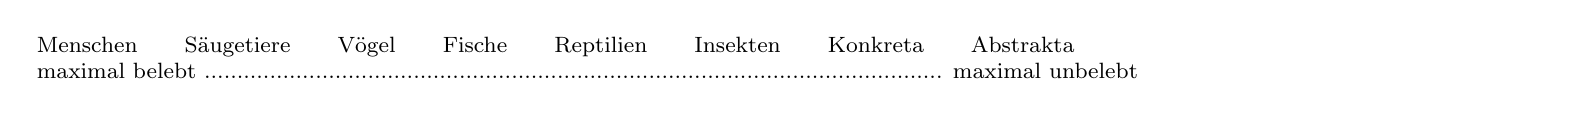
\begin{tikzpicture}[
squarednode/.style={rectangle, minimum size=1mm, font=\footnotesize}]
\node[squarednode]      (noun)       {\parbox{19cm}{Menschen  \ \ \ \ \  Säugetiere \ \  \ \ \ Vögel \ \ \  \  \ Fische  \ \ \ \ \   Reptilien  \  \ \ \   \ Insekten  \ \ \ \   \ Konkreta   \ \ \ \  \ Abstrakta \\
maximal belebt ................................................................................................................. maximal unbelebt}};
\end{tikzpicture}
\caption{Belebtheitsskala nach \textcite[115]{Kopcke.2000}}
\label{fig2l}
\end{figure}

Mit einem Hund hat der Mensch mehr Gemeinsamkeiten als mit einer Biene, die statt vier sechs Extremitäten hat (\cite[94]{Flick.2020}). Zudem sind einzelne Bienen weniger gut unterscheidbar als einzelne Hunde. Da Bienen als Schwarmtiere prototypischerweise in der Mehrzahl auftreten, ist die Individuiertheit außerdem aufgrund der Pluralität herabgesetzt. Daher werden Hunde eher als Individuen wahrgenommen als Bienen. 

Der hohe Belebtheitsgrad von schwachen Maskulina kann als Erklärung für die unterschiedliche Markierung von Nominativ und obliquen Kasus in der Deklination schwacher Maskulina genutzt werden (\cite[117--118]{Kopcke.2000}). Der Nominativ markiert prototypischerweise das Subjekt und diese syntaktische Funktion korreliert meist mit der semantischen Rolle des Agens (\cite[118]{Kopcke.2000}). Diese Rolle ist prototypischerweise mit Entitäten besetzt, die handlungsfähig sind und somit einen hohen Belebtheitsgrad aufweisen (\cite[248]{Langacker.1991}, \cite[16--17]{Primus.2012}, \cite[103--104]{Flick.2020}).\footnote{Die Rolle des Agens kann auch mit nicht-belebten Entitäten besetzt sein, dies ist aber nicht die prototypische Besetzung derselben, siehe hierzu genauer \textcite[114--115]{Flick.2020}.} Aufgrund der Korrelation zwischen Belebtheit, Agens und Nominativ ist es für Substantive mit hohem Belebtheitsgrad sinnvoll, die Agensrolle im Gegensatz zu den anderen semantischen Rollen unmarkiert zu lassen (\cite[118]{Kopcke.2000}): Da Entitäten mit hohem Belebtheitsgrad potentiell handlungsfähig sind, ist es generell wahrscheinlich, dass sie Agens einer Handlung sind. Daraus folgt, dass die semantischen Rollen gesondert markiert werden, bei denen diesen Entitäten unerwarteterweise keine handlungstragende Funktion zukommt. Die auffällige Markierung der Dativ- und Akkusativformen ist aus dieser Perspektive eine Konsequenz der Belebtheit schwacher Maskulina. Diese Hypothese überprüfen \textcite{Binanzer.2020b}: Sie präsentieren in einer Eye-Tracking-Studie Sätze in SVO- und OVS-Abfolge mit starken und schwachen Maskulina. In der Studie wurden die Sätze auditiv präsentiert und Bilder gezeigt, die in Beziehung zum Sprachmaterial standen (Bei \textit{Welcher Arzt beobachtet die Frau?} und \textit{Welchen Arzt beobachtet die Frau?} waren Figuren zu sehen, die man leicht als Arzt bzw. als eine weibliche Person identifizieren konnte). Erwachsene Proband\_innen konnten die Sätze und das Bildmaterial erfolgreicher verknüpften, wenn schwache Maskulina anstatt starker als Patiens genutzt wurden, bei Kindern zeigte sich dies nur in der SVO-Abfolge (\cite[399]{Binanzer.2020b}). Obwohl die Markierung durch den Determinierer erfolgt, scheint somit die gesonderte Markierung der Patiensrolle zu einem Prozessierungsvorteil zu führen. Hier lässt sich wiederum das Konzept der Relevanz anführen: Für belebte Entitäten ist die Opposition zwischen Nominativ und obliquen Kasus aufgrund der möglichen semantischen Rollen relevanter, weshalb diese direkt am Substantiv markiert werden.

Wie bei den starken und schwachen Verben stehen sich auch bei schwachen und starken Substantive eine schlecht generalisierbare, weil auf wenige und wenig variable Substantive beschränkte, und eine hochschematische Deklinationsklasse gegenüber. Dies lässt sich vorrangig für den Singular postulieren. Für den Plural ist die Lage komplexer, da nicht nur -\textit{(e)n} und -\textit{e} möglich sind, sondern auch weitere Suffixe. Die folgenden Ausführungen fokussieren auf den Singular. Anders als bei den Form-Schemata der starken Verben sind bei dem Form-Schema der schwachen Maskulina nicht nur prosodisch-phonologische Eigenschaften (Dreisilbigkeit, Pänultimabetonung, Schwa) mit einem bestimmten Flexionsverhalten verknüpft, sondern auch eine semantische (Belebtheit). Dies lässt sich gut durch einen Zweischritt modellieren, wie Abbildung \ref{Schematyp} zeigt. 

\begin{figure}
\includegraphics[width=\textwidth]{figures/Kap4/schemaI,II.png}  
\caption{Verschachtelung des Form-Schemas bei schwachen Maskulina}
\label{Schematyp}
\end{figure}

Zunächst ist von einer teilschematischen Konstruktion auszugehen, die die Form [dreisilbig, pänultimabetont, \mbox{Schwa-En}\-dung] mit der Funktion [+menschlich] assoziiert.  Diese Konstruktion ist Teil des Form-Schemas: Die Eigenschaften [dreisilbig, pänultimabetont, Schwa-Endung, +~menschlich] sind mit schwachem Flexionsverhalten verknüpft. Das Form-Schema ist in diesem Fall also komplex verschachtelt, da nicht nur die Verknüpfung von einzelnen Flexionsformen mit einzelnen Funktionen gemeinsam eine Assoziation von Form auf Lexemebene und Flexionsverhalten ergeben (siehe hierzu genauer \sectref{steuerungschema}), sondern die Form zusätzlich eine teilschematische Konstruktion darstellt. 

Insgesamt lässt sich festhalten, dass die Klasse der schwachen Maskulina komplex konditioniert ist, da semantische, prosodische sowie phonologische Faktoren\footnote{Wenn man das finale Schwa als Belebtheitsmarker interpretiert, ist die Klassenzugehörigkeit zusätzlich morphologisch konditioniert (\cite[172]{Nubling.2016}).} die Klassenzugehörigkeit beeinflussen (\cite[172]{Nubling.2016}). In den folgenden Abschnitten~\ref{sch1} und \ref{sch2} werden die prototypische Organisation und der Einfluss der Form-Schemata auf die Fle\-xion von Maskulina näher in den Blick genommen. Dabei wird mit \textit{Form-Schema I} auf das Form-Schema mit den Eigenschaften [Dreisilbigkeit, Pänultimabetontung, Schwa-Endung, +~menschlich] referiert, mit \textit{Form-Schema II} auf das Form-Schema mit den Eigenschaften [Dreisilbigkeit, Ultimabetonung, +~menschlich].  



\subsubsection{Form-Schema I}  \label{sch1}

Der phonologischen Form [Dreisilbigkeit, Pänultimabetontung, Schwa-Endung] entsprechen gut 80 native Substantive, hinzu kommen etwa 200 nicht-native Substantive (\cite[171]{Kopcke.1995}). Die meisten Substantive mit dieser Form haben einen hohen Belebtheitsgrad: Nur ein Substantiv (\textit{Gedanke}) referiert auf eine abstrakte Entität und weitere fünf auf belebte, aber nicht-menschliche Entitäten (bspw. \textit{Schimpanse}). \textit{Gedanke} zeigt allerdings bereits Übergangstendenzen zur starken Deklinationsklasse: Der Genitiv wird auf -\textit{ns} gebildet (\textit{des Gedankens}) und laut \textcite[171]{Kopcke.1995} existiert auch die \textit{n}-haltige Nominativform (\textit{der Gedanken}).\footnote{Woran er diese Aussage festmacht, erläutert \textcite{Kopcke.1995} jedoch nicht.} Die restlichen dreisilbigen Substantive auf Schwa referieren auf menschliche Entitäten. Dreisilbigkeit, Pänultimabetontung und Schwa-Endung scheinen also stark mit einem hohen Belebtheitsgrad assoziiert zu sein und damit eine hohe \textit{cue validity} zu haben (zum Konzept der \textit{cue validity} siehe \sectref{standard}). 

 

\textcite[395--396]{Schafer.2019} geht davon aus, dass die prosodisch-phonologischen Eigenschaften eine höhere Salienz haben und somit stärker zur Profilierung der schwachen Maskulina beitragen als die semantischen, da ein hoher Belebtheitsgrad nicht automatisch zur schwachen Flexion führt (*\textit{des Fischern}). Zudem weist er darauf hin, dass die dreisilbigen Substantive mit Pänultimabetonung von den typischen prosodisch-phonologischen Eigenschaften deutscher Substantive (monosyllabisch oder trochäisch) abweichen und daher salient sind. 

Form-Schema I ist produktiv: So werden Einwohnerbezeichnungen nach diesem Form-Schema gebildet und schwach flektiert, wie bspw. \textit{der Kasache} (\cite[112]{Kopcke.2000}). Ein weiteres Indiz für die Produktivität des Form-Schemas liefern Substantive auf -\textit{or} (\textit{der Autor}): Diese gehören der gemischten Klasse an, da sie den Singular stark bilden, den Plural jedoch auf -\textit{en}. Die Pluralformen auf -\textit{en} machen aus der Anfangsbetonung (\textit{Áutor}) eine Pänultimabetonung (\textit{Autóren}). Im Plural entsprechen  Bildungen auf -\textit{or} also der phonologischen Form des Form-Schemas I. Zudem passt \textit{der Autor} aufgrund seines hohen Belebtheitsgrads in das Form-Schema~I. \textcite[78]{Kopcke.2005} sieht darin den Grund dafür, dass dieses Substantiv vereinzelt auch im Singular schwach dekliniert wird (\textit{des Autoren} statt \textit{des Autors}). In seiner Google-Untersuchung liegen die schwachen Belege allerdings lediglich bei 1 \% bis 5 \%. Nur bei \textit{Juror} sind sie mit 17~\% häufiger vertreten. Die empirischen Befunde scheinen somit nur auf einen kleinen Effekt hinzudeuten. \textcite[406--407]{Schafer.2019} kann in seiner Korpusstudie zeigen, dass Belebtheit dabei eine Rolle spielt: Substantive auf -\textit{or} werden mit menschlichen Referenten eher schwach dekliniert als mit unbelebten Referenten. Interessanterweise wird der Genitiv bei diesen Substantiven laut Schäfer häufiger schwach dekliniert als Dativ und Akkusativ. Die Substantive auf -\textit{or} verhalten sich also invers zu den schwachen Maskulina, die zur starken Flexion schwanken (siehe hierzu genauer \sectref{protmask}).   



\textcite[169]{Kopcke.1995} sieht in Entlehnungen, die dem Form-Schema~I der schwachen Maskulina ähnlicher gemacht wurden, ein weiteres Indiz für dessen Produktivität: Bei \textit{Mormone} und \textit{Schamane} wurde der ursprüngliche Wortakzent weg von der Erstsilben- hin zur Pänultimabetonung verschoben, außerdem haben die Substantive Schwa angenommen: \textit{mórmon} > \textit{Mormóne} (\cite[169]{Kopcke.1995}). Auch native Substantive nehmen Schwa an, um in der schwachen Flexion zu bleiben: \textit{der Vor}-/\textit{Nachfahr} > \textit{der} \textit{Vor}-/\textit{Nachfahre} (\cite[137--138]{Kopcke.1993}), allerdings führt dies nicht zu einer Akzentverschiebung (\textit{der Vórfahre}). Laut \textcite[113--115]{Kusova.2014} ist bei \textit{Vorfahr(e)} die Form auf Schwa im Deutschen Referenzkorpus mit 67~\% frequenter als die schwa-lose. Bei \textit{Exot(e)} stellt sie hingegen eine klare Tendenz zur Form ohne Schwa fest. Durch die Ultimabetonung (\textit{Exót}) passt das Substantiv bereits zu Form-Schema~II, daher ist ein Annehmen von Schwa wie bei \textit{Mormone} nicht nötig, um mit schwachem Flexionsverhalten assoziiert zu werden. 


Die Abkopplung des Form-Schemas~II für schwache Maskulina durch Schwa-Apokope zeigt, dass neben der Annahme von Schwa auch der Wegfall möglich ist. Dies lässt sich bei einigen Entlehnungen nachverfolgen: \textit{Bojare} > \textit{Bojar} (\cite[168]{Kopcke.1995}). Auch hier entsteht eine Ultimabetonung, sodass das Substantiv zu Form-Schema~II passt.

Form-Schema I ist prototypisch organisiert. Während nur knapp 300 Substantive die prototypische Form aufweisen, zählen inklusive der Peripherie ca. 500 Substantive zum Form-Schema~I (\cite[98--99]{Bittner.20031991}). Dabei existieren sowohl ein prosodisch-phonologischer Prototyp (Dreisilbigkeit, Pänultimabetontung und \mbox{Schwa-En}\-dung) und eine prosodisch-phonologische Peripherie (Monosyllabizität) als auch ein semantischer Prototyp (Mensch) und eine semantische Peripherie (Unbelebtheit). Abbildung \ref{fig2lnm} stellt die Abstufungen schematisch dar.

\begin{figure}
\includegraphics[width=\textwidth]{figures/Kap4/PrototypIneu.png}  
\caption{Abstufungen des Form-Schemas dreisilbig, pänultimabetont, Schwa-Endung, menschlich; angelehnt an \textcite[170]{Kopcke.1995}}
\label{fig2lnm}
\end{figure}

Einen Schritt von der prototypischen phonologischen Form [dreisilbig, pänultimabetont, Schwa-Endung] entfernt sind Substantive, die zweisilbig sind und auf Schwa auslauten: \textit{Júnge}, \textit{Bóte}.\footnote{Da sich die Pänultimabetonung aus der Zweisilbigkeit und der Schwa-Endung ergibt, wird sie nicht als gesonderte Eigenschaft gesehen, auch wenn sie bei \textcite[113]{Kopcke.2000} als Eigenschaft aufgeführt wird.} \textcite[171]{Kopcke.1995} schreibt der zweisilbigen Form nur bedingte Produktivität zu und nennt als Neuzugang lediglich \textit{der Kurde}. Zudem führt die phonologische Form [Zweisilbigkeit und Schwa-Endung] auch in Kombination mit einem hohen Grad an Belebtheit nicht zwangsläufig zur schwachen Deklination: \textcite[172]{Kopcke.1995} nennt \textit{Piefke}, \textit{Steppke} und \textit{Vize} als potentielle Vertreter des Form-Schemas~I, die dennoch starke Flexion aufweisen. Für \textit{Piefke} und \textit{Steppke} nimmt \textcite[172]{Kopcke.1995} an, dass die pejorative Bedeutung die Deklination beeinflusst.\footnote{Zusätzlich könnte das Diminutivsuffix -\textit{ke} bei \textit{Piefke} und \textit{Steppke} eine Assoziation mit dem Form-Schema~I erschweren. \textit{Vize} ist ein Kurzwort, das sich erst im 19. Jahrhundert aus Komposita wie \textit{Vizekanzler} herausbildet (\cite[1520]{Pfeifer.2000}). Die späte Entstehung und der Status als Kurzwort könnten die schwache Flexion blockieren.}  



Dennoch stellt sich generell die Frage, ob es gerechtfertigt ist, für drei- und zweisilbige Substantive einen Unterschied in der Typizität anzunehmen. M.~E. ist die Abstufung aus theoretischer Sicht sinnvoll: Da nur wenige Substantive mit den phonologisch-prosodischen Eigenschaften [dreisilbig, pänultimabetont und Endung auf Schwa] auf Entitäten referieren, die nicht menschlich sind, kommt dieser Form eine höhere \textit{cue validity} zu als der Form [zweisilbig und Endung auf Schwa]. Allerdings scheint dies keine praktischen Auswirkungen zu haben. Abbautendenzen der schwachen Flexion zeigen sich sowohl bei den dreisilbigen als auch bei den zweisilbigen Substantiven nur in Kombination mit geringer Belebtheit. Daher sind Schwankungen bei Abstrakta, Konkreta und Substantiven, die auf Vögel, Fische, Reptilien und Insekten referieren, zu beobachten und diachron nachzuvollziehen (\cite[112--117]{Kopcke.2000}). Eine Ausnahme von der belebheitsgesteuerten Klassenzugehörigkeit ist \textit{die Waise}, ein Substantiv, dessen Referent einen hohen Belebtheitsgrad aufweist, das aber dennoch von der schwachen maskulinen (\textit{der Waise}) in die feminine Deklination gewechselt ist (\cite[116--117]{Kopcke.2000}). Auch \textit{der Falke}, der sich bislang in der schwachen Flexion halten konnte, erscheint auf den ersten Blick als Ausnahme, da er auf einen Vogel referiert. Falken kam jedoch im Mittelalter ein hoher kultureller Stellenwert und damit ein höherer Belebtheitsgrad als anderen Vögeln zu (\cite[112--113]{Kopcke.2000}).  

Für zweisilbige Substantive mit geringem Belebtheitsgrad lassen sich zwei Entwicklungslinien festhalten: Wie dreisilbige Substantive mit geringem Belebtheitsgrad nehmen sie im Genitiv -\textit{ns} und in der Folge -\textit{n} an (ausführlich hierzu siehe \sectref{protmask}), zudem können sie das Genus wechseln. \textit{Der Krake} zeigt momentan beide Entwicklungstendenzen: Einerseits schwankt das Substantiv im Genitiv zwischen -\textit{n} (\textit{des Kraken}) und -\textit{ns} (\textit{des Krakens}) und tendiert dazu, im Nominativ -\textit{n} anzunehmen (\textit{der Kraken}) und somit in die starke Deklination überzugehen, andererseits finden sich feminine Formen (\textit{die Krake}). \textcite[224--227]{Kopcke.2018} stellen hierbei Bedeutungsdifferenzierungen fest: \textit{die Krake} wird vorrangig metaphorisch verwendet (\textit{die Datenkrake}), während \textit{der Krake} vorrangig auf das Tier verweist. 

 



Tendenzen zur Annahme von -\textit{n} im Nominativ lassen sich außerdem bei \textit{der Name/n}, \textit{der Wille/n} und \textit{der Buchstabe/n} beobachten (\cite[173]{Kopcke.1995}). Bei \textit{der Friede/n} sieht \textcite[173]{Kopcke.1995} den Prozess als abgeschlossen an. Auch diachron zeigen sich Beispiele von \textit{n}-Annahmen im Nominativ: \textcite[113--115, 120]{Kopcke.2000} führt 72 Maskulina auf wie bspw. \textit{Rücken}, \textit{Hopfen} und \textit{Weizen}, die ursprünglich auf Schwa auslauteten. Schwankungen in der Nominativform können ebenfalls mit einer Bedeutungsdifferenzierung einhergehen: So ist \textit{der Drache} ein feuerspeiendes Wesen, während \textit{der Drachen} steigen gelassen werden kann (\cite[173]{Kopcke.1995}). Genauso werden für \textit{Funke/n} Bedeutungsunterschiede diskutiert: Die Bedeutung \SchmittSingleQuot{geringes Ausmaß} (\textit{ein Funken Hoffnung}) ist laut \textcite[403]{Sandberg.1998} auf die \textit{n}-haltige Nominativform beschränkt. \textcite[316--317]{Joeres.1996} sieht indes keinen semantischen Unterschied zwischen \textit{n}-haltigen und \textit{n}-losen Formen bei \textit{Funke}. Für \textit{der} \textit{Friede/n} werden ebenfalls Bedeutungsdifferenzierungen diskutiert: In der Bedeutung \SchmittSingleQuot{Nicht-Kriegszustand} wird laut \textcite[336]{Duden.2016} die \textit{n}-haltige Nominativform bevorzugt, während \textit{der Friede} in der religiösen Bedeutung \SchmittSingleQuot{Geborgenheit in Gott} genutzt wird. Auf eine mögliche Bedeutungsdifferenzierung geht \textcite[313--316]{Joeres.1996} nicht ein, er merkt lediglich an, dass viele \textit{n}-lose Belege Redensarten aus der Bibel darstellen. 
Auch der umgekehrte Weg zur \textit{n}-Annahme im Nominativ -- die Tilgung von -\textit{n} -- lässt sich diachron feststellen. Diese führte dazu, dass ehemals starke Substantive zu schwachen wurden. Dies ist nur bei Substantiven mit hohem Belebtheitsgrad zu beobachten wie bspw. bei \textit{Schöffe} < mhd. \textit{scheffen} und \textit{Heide} < mhd. \textit{heiden} (\cite[112]{Kopcke.2000}).

\begin{sloppypar}
Der Genuswechsel von schwachen Maskulina zu Feminina  lässt sich durch Form-Schemata erklären: Die Form [Zweisilbigkeit und Schwa] deckt sich im Nominativ Singular mit den phonologischen Eigenschaften schwacher Feminina (\textit{die Wólke}). Zudem ist die Pluralmarkierung auf -\textit{(e)n} prototypisch für gemischt-deklinierte Feminina (\cite[115]{Kopcke.2000}). Es ist daher ein alternatives Form-Schema verfügbar, an das sich die Substantive anschließen können, deren Referenten einen geringen Belebtheitsgrad aufweisen. Der Einfluss des finalen Schwas auf die Genuswahl wird auch anhand von Minimalpaaren deutlich, die sich allein in der Existenz des Schwa unterscheiden: \textit{die Quelle} vs. \textit{der Quell}, \textit{die Zehe} vs. \textit{der Zeh} (\cite[168]{Nubling.2016}).\ \textcite[128]{Kopcke.1993} sieht die Schwa-Endung daher als Genusindikator. Hinsichtlich der Schwa-Endung wird zudem angenommen, dass sie Belebtheit markieren kann (\cite[75]{Kopcke.2005}). Inwiefern sich diese Funktionen des Schwa widersprechen und inwiefern sie vereinbar sind (Schwa als Marker für Feminina, Schwa bei Maskulina dagegen als Belebtheitsmarker) wurde in der Forschung meines Wissens nicht diskutiert. 
\end{sloppypar}


Unabhängig vom Status des Schwa kann festgehalten werden, dass zweisilbige Substantive auf Schwa zur Form zweier Form-Schemata passen. Auch hier ist von zwei Ebenen auszugehen: Zweisilbigkeit und Schwa-Endung können sowohl mit menschlichen als auch mit nicht-menschlichen Referenten assoziiert sein. Auf der übergeordneten Ebene entscheidet daher die Belebtheit darüber, welches Form-Schema greift und welches Genus genutzt wird, siehe Abbildung \ref{femmask}.\footnote{Innerhalb der Belebtheit beeinflusst Sexus die Assoziation mit schwachen Maskulina bzw. Feminina. So gehören Substantive wie \textit{die Tante} und \textit{die Nichte} aufgrund des Sexus zu den Feminina und nicht zu den schwachen Maskulina.} 

\begin{figure}
\includegraphics[width=\textwidth]{figures/Kap4/femmask.png}  
\caption{Verschachtelung der Form-Schemata von schwachen Maskulina und Feminina}
\label{femmask}
\end{figure} 

Der Genuswechsel von zweisilbigen schwachen Maskulina auf Schwa mit geringer Belebtheit hin zu den Feminina lässt sich als Profilierung der Form-Sche\-ma\-ta werten: Im Fall von \textit{Krake} korreliert eine geringe Belebtheit mit der Funktion [+maskulin]. Durch den Genuswechsel zu [+feminin] wird die \textit{cue validity} des Form-Schemas der schwachen Maskulina sowie der gemischt-deklinierten Feminina gestärkt und beide Form-Schemata daher profiliert. 

 

Eine vergleichbare Profilierung lässt sich für den Wechsel zur starken Deklination durch Annahme von -\textit{n} ansetzen: Zwei- und dreisilbige Substantive mit geringem Belebtheitsgrad sind nur wenig mit schwacher Flexion assoziiert. Durch die Annahme von -\textit{n} wird die Assoziation weiter gesenkt, da nun auch die prosodisch-phonologischen Eigenschaften der Form aufgrund des fehlenden Schwa-Auslauts nicht mehr erfüllt werden. Hierdurch sind Substantive wie \textit{der Kraken} weder mit den semantischen noch mit den prosodisch-phonologischen Eigenschaften des Form-Schemas kompatibel und werden daher auch nicht mit schwacher Flexion assoziiert. 

Welche Faktoren dazu führen, dass zweisilbige Substantive mit geringem Belebtheitsgrad die Deklinationsklasse oder das Genus wechseln, ist meines Wissens bislang nur in Ansätzen erforscht. Einerseits könnte Pluralität eine Rolle spielen: Für Entitäten, auf die häufig im Plural referiert wird, ist eine Pluralopposition relevant. Diese wird durch den Genuswechsel ermöglicht (\cite[305]{Nubling.2008}). Die Numerusprofilierung kann daher als Erklärung für den Genuswechsel von Schwarmtieren wie Heuschrecken herangezogen werden sowie von paarigen Körperteilen wie \textit{die Niere}, die aufgrund ihrer Paarigkeit häufiger im Plural verwendet werden als im Singular (\cite[305]{Nubling.2008}). 



Andererseits können semantische Rollen für die Entwicklung relevant sein. Wird ein Substantiv häufig als Subjekt in Passivsätzen und der Nominativ somit in der Patiensrolle gebraucht, könnte dies dazu führen, dass die \textit{n}-haltige Form, die auf Kasus in Nicht-Agens-Rollen beschränkt ist, auf den Nominativ ausgeweitet wird:\footnote{Für diesen Hinweis danke ich Melitta Gillmann.} Aus \textit{der Weize} wird also \textit{der Weizen}, weil \textit{Weizen} nun einmal geerntet wird und nicht selbst erntet. Dieser Erklärungsansatz deckt sich mit der diachronen Entwicklung, in der vornehmlich Konkreta und Abstrakta \textit{n}-haltige Nominative annahmen (\cite[120]{Kopcke.2000}). Konkreta und Abstrakta sind aufgrund ihres geringen Belebtheits- sowie Individuiertheitsgrads nur eingeschränkt als Agens nutzbar. Im Einzelfall lässt sich dennoch nicht immer nachvollziehen, warum welcher Weg eingeschlagen wurde. So hat \textit{die Hirse} das Genus gewechselt, während andere Getreidesorten und getreideähnliche Pflanzen wie bspw. \textit{Roggen}, \textit{Weizen} und \textit{Hopfen} \textit{n}-haltig geworden sind (\cite[120--121]{Kopcke.2000}).     

Variation zwischen \textit{n}-haltigen und endungslosen Dativ- und Akkusativformen (\textit{dem/den Krake/n}) oder zwischen Genitivformen auf -\textit{n} und -\textit{s} (\textit{des Kraken/s}) lässt sich für drei- und zweisilbige Substantive auf Schwa nicht feststellen. Die \textit{n}-haltigen Nominativformen und die Feminina stechen diese Entwicklungsmöglichkeit statistisch aus, da mehr Substantive mit ähnlichen phonologischen Eigenschaften und ähnlicher Semantik existieren, die entweder -\textit{n} im Nominativ enthalten oder Feminina sind. Dies zeigt sich bspw. bei den Genitivformen: Es existieren viele zweisilbige Substantive auf Schwa mit Genitiv auf -\textit{ns} bspw. aufgrund von substantivierten Verben (\textit{des Tragens, des Lachens}), aber nur wenige mit Genitiv auf -\textit{s} (\textit{des Käses}) (\cite[71]{Kopcke.2005}). Formen auf -\textit{ns} sind somit bei zwei- und dreisilbigen Maskulina typenfrequenter und daher konventioneller. 

Monosyllabische Substantive\footnote{\textcite[60--61]{Krischke.2012} setzt vor den monosyllabischen Substantiven eine weitere Abstufung des Form-Schemas an: zweisilbige Substantive mit Pänultimabetonung, aber ohne Schwa. Als Beispiele nennt er \textit{Bauer}, \textit{Nachfahr} und \textit{Vorfahr}. Diese Substantive schwanken in ihrer Verwendung: \textit{Bauer} schwankt zur starken Flexion (\cite[132--133]{Duden.2016}), bei \textit{Nach}- und \textit{Vorfahr} finden sich wie oben diskutiert schwa-haltige Nominativformen (\textit{der Nachfahre}) (\cite[137--138]{Kopcke.1993}). Zwar ist \textit{Bauer} nicht schwa-haltig, es enthält aber mit dem vokalisierten R einen Reduktionsvokal. Bei \textit{nach} und \textit{vor} in \textit{Nach}- bzw. \textit{Vorfahr} handelt es sich um Präfixe. Anders als \textit{Junge} und \textit{Bauer} sind \textit{Vor}- und \textit{Nachfahr} somit komplexe morphologische Wörter. Der Stamm (-\textit{fahr}) ist nicht zweisilbig, sondern lediglich das Wortbildungsprodukt.} sind aufgrund ihrer prosodisch-pho\-no\-lo\-gisch\-en Eigenschaften nicht mit schwacher Flexion assoziiert, da viele Einsilber stark flektieren wie bspw. \textit{der Stuhl} und \textit{der Stein}. Allein ein hoher Belebtheitsgrad kann hier die schwache Flexion bewahren. Aber auch Substantive mit hohem Belebtheitsgrad (\textit{Prinz, Graf}) zeigen Schwankungen hin zur starken Flexion: Im Dativ und Akkusativ finden sich endungslose Formen (\textit{den/dem Graf∅}), im Genitiv sind Formen auf  -\textit{s} (\textit{des Grafs}) sowie vereinzelt Formen auf -\textit{(e)ns} (\textit{des Grafens}) zu beobachten.\footnote{\textcite[76--77]{Krischke.2012} beobachtet, dass Genitivformen auf -\textit{(e)ns} bei monosyllabischen Substantiven bereits im 13. Jahrhundert unabhängig vom Belebtheitsgrad der Referenten auftauchten: \textit{des Affens}, \textit{Botens}, \textit{Prinzens}. Allerdings scheinen sich diese Formen bei keinem der von \textcite[76--77]{Krischke.2012} genannten Beispiele durchgesetzt zu haben.} Bei monosyllabischen Substantiven, die auf Unbelebtes referieren (bspw. \textit{Stern}, \textit{März}), ist der Prozess abgeschlossen. Die schwachen Formen sind nur noch in Komposita und Redewendungen fossilisiert (\textit{Stern\textbf{en}himmel}, \textit{Im März\textbf{en} der Bauer}). 

\begin{sloppypar}
\textcite[114--115]{Kopcke.2000} beschreibt eine belebtheitsgesteuerte Entwicklung der ursprünglich schwach deklinierten monosyllabischen Substantive: Während 27~\% der Substantive mit menschlichen Referenten die schwache Flexion beibehielten (\textit{der Herr}, \textit{der Fürst}), sind es bei tierischen Referenten nur rund 13 bis 17 \% (\textit{der Fink}); Entitäten mit geringerem Belebtheitsgrad sind komplett in die starke Flexion gewechselt (\textit{der Mai}). \textcite[114--115]{Kopcke.2000} betrachtet nur Substantive, die das stammfinale Schwa vom Mhd. zum Frnhd. apokopierten und hierdurch in die Peripherie der schwachen Substantive gelangt sind.\footnote{\textcite[120--121]{Kopcke.2000} beruft sich in seiner Auflistung auf die Grammatik von \textcite{Paul.1917}. Köpckes Daten sind jedoch mit Vorsicht zu genießen, denn in Köpckes Liste sind auch Substantive wie \textit{Apt} und \textit{Dieb}, die im Mittelhochdeutschen Handwörterbuch von \textcite{Lexer.18721878} lediglich als starke Maskulina geführt werden. Die aufgeführten Formen (u.a. \textit{abbet}, \textit{abt}, \textit{diup}, \textit{diep}) sind zudem allesamt nicht schwa-haltig. Mhd. \textit{karl(e)} (nhd. \textit{Kerl}) wird als schwaches sowie starkes Maskulinum ausgewiesen. Außerdem sind in der Grammatik von \textcite{Paul.1917} nicht alle von \textcite{Kopcke.2000} untersuchten Substantive als schwach flektierend aufgeführt. Einige sind als Substantive klassifiziert "`von denen sw. Formen vorkommen"' (\cite[46]{Paul.1917}). Dazu zählen auch \textit{Apt} und \textit{Dieb}. Die im Fließtext angeführten Beispiele wurden dahingehend überprüft, ob sie im Mittelhochdeutschen Handwörterbuch als auf Schwa auslautendes schwaches Maskulinum geführt werden.}  
\end{sloppypar}


Auch für das Neuhochdeutsche kann der Einfluss der prosodisch-pho\-no\-lo\-gisch\-en und semantischen Eigenschaften des Form-Schemas~I auf die Flexion nachgewiesen werden. In einem Produktionsexperiment zeigt \textcite[77--78]{Kopcke.2005}, dass Schüler\_innen der Jahrgangsstufe 6 vor allem bei monosyllabischen Substantiven die starke Deklination bevorzugen. Bei zweisilbigen Substantiven auf Schwa überwiegt hingegen die schwache Flexion, das dreisilbige Substantiv wird exklusiv schwach dekliniert. Dabei spielt auch Belebtheit eine Rolle, denn \textit{der Bote} wird zu 100 \% schwach flektiert, \textit{der Falke} nur zu 75 \%. Ähnliche Belebtheitseffekte lassen sich für die monosyllabischen Substantive feststellen (\cite[77]{Kopcke.2005}). Insgesamt ist die schwache Flexion bei den zweisilbigen Formen aber unabhängig von der Belebtheit stabiler als bei den monosyllabischen Substantiven. Dies bestätigt die Hypothese von \textcite[394--396]{Schafer.2019}, nach der prosodisch-phonologische Eigenschaften die Flexion besser stützen als die semantische. Auch \textcite{Schafer.2019} kann im Rahmen seiner Korpusuntersuchung mithilfe einer logistischen Regression das Wirken des von \textcite{Kopcke.1995} postulierten prosodisch-phonologisch und semantisch motivierten Form-Schemas bestätigen.

Weitere Hinweise auf das Wirken des Form-Schemas I liefert ein Produktionsexperiment von \textcite{Kopcke.2000b}. 31 Proband\_innen\footnote{Bei allen Proband\_innen handelte es sich um Germanistikstudent\_innen am Anfang des Studiums (\cite[159]{Kopcke.2000b}).} wurden hierfür Pseudosubstantive präsentiert, zu denen ihnen nur das Genus und die Bedeutung genannt wurden. Die Proband\_innen wurden gebeten, die Testsubstantive in den Genitiv Singular sowie Nominativ Plural zu setzen (\cite[159]{Kopcke.2000b}). Die Substantive sind dreisilbig  mit Pänultimabetonung und Schwa (z.~B. \textit{Schéttose}), zweisilbig mit Schwa (z.~B. \textit{Zirfe}) oder monosyllabisch (z.~B. \textit{Knatt}), sodass sie in ihren prosodisch-phonologischen Eigenschaften gestaffelt und damit zu unterschiedlichen Graden mit schwachen Maskulina assoziiert sind. Die ein- und zweisilbigen Testitems  sind zusätzlich mit unterschiedlichen Belebtheitsgraden versehen: \textit{Der Zirfe} wird bspw. als hoher türkischer Würdenträger eingeführt, während \textit{der Stisse} als ein dem Zebra ähnliches Tier definiert wird (\cite[168]{Kopcke.2000b}). Zusätzlich nutzt \textcite{Kopcke.2000b} Substantive auf -\textit{or} sowie Substantive auf -\textit{el} bzw. -\textit{er} als Testwörter.\largerpage



Mit diesem Design kann \textcite[159--166]{Kopcke.2000b} den Einfluss des Form-Sche\-mas~I auf die Deklination von Maskulina beobachten. Die Häufigkeit der schwachen Flexion nimmt von der dreisilbigen hin zur einsilbigen Form ab: Während die dreisilbigen Substantive zu 76 \% -\textit{(e)n} im Genitiv aufweisen, sind es bei den monosyllabischen 9~\% (unbelebt) bis 39~\% (menschlich).\footnote{\textcite[416--418]{RonnebergerSibold.2020} kann in einer Replikationsstudie mit Studierenden aus Bayern, deren Sprachverhalten stark dialektal geprägt ist, jedoch keine Präferenz für -\textit{s} oder \mbox{-\textit{n}} bei \textit{Schettose} ablesen. Sie erklärt diesen Befund damit, dass der Genitiv in Dialekten gemieden wird und sich somit das Form-Schema schwacher Maskulina nicht festigen kann.} Die Abstufungen innerhalb der einsilbigen Testsubstantive verdeutlichen den Einfluss der Belebtheit. Dieser zeigt sich auch bei zweisilbigen Substantiven: Korreliert Zweisilbigkeit mit einem hohen Grad an Belebtheit, nimmt die Tendenz zur schwachen Flexion im Vergleich zur dreisilbigen Form nur leicht ab (61 \%). Wird dagegen auf tierische Entitäten referiert, fällt die Anzahl schwach gebildeter Genitive auf 37~\% und gleicht damit dem Anteil schwacher Maskulina bei einsilbigen Substantiven mit hohem Belebtheitsgrad.  



Die Substantive auf -\textit{or} weisen mit 27~\% einen ähnlichen Anteil an schwachen Genitivformen auf wie die Einsilbler mit tierischen Referenten. Aber auch hier ist der Einfluss der Belebtheit zu erkennen: Während das Pseudosubstantiv \textit{Frátor}, das als [+menschlich] eingeführt wurde, zu 32~\% im Genitiv schwach flektiert wird, wird \textit{Tréitor} mit nicht-belebter Referenz nur zu 22~\% schwach flektiert. Wie bei dem real existierenden Substantiv \textit{Autor} zeigt sich hier die Anziehungskraft des Form-Schemas~I. 



\textcite[159--161]{Kopcke.2000b} stellt die Hypothese auf, dass der Anteil der schwachen Deklination bei Substantiven auf -\textit{el} und -\textit{er} am geringsten ist, da Substantive auf -\textit{el} und -\textit{er} beinahe ausnahmslos stark deklinieren.\footnote{\textcite[160--161]{Kopcke.2000b} schätzt, dass 3~\% der Substantive auf -\textit{el} und -\textit{er} schwach deklinieren. Bei dieser Schätzung sind durchsichtige Derivationen auf -\textit{er} (\textit{fischen} > \textit{der Fischer}) allerdings ausgeschlossen, sodass der tatsächliche Anteil sogar geringer ist.}  Die Hypothese bestätigt sich: Die Substantive auf -\textit{el} oder -\textit{er} weisen mit 87~\% vornehmlich starke Genitivformen auf (\cite[161]{Kopcke.2000b}). Substantive auf -\textit{er} und -\textit{el} lassen sich daher als Form-Schemata der starken Deklination betrachten.\footnote{Das Form-Schema der starken Maskulina ist vergleichbar mit dem Form-Schema regelmäßiger Verben im Englischen: Englische Verben auf /f/ flektieren regelmäßig (\textit{to laugh}, \textit{laughed}) (\cite[135]{Goldberg.2019}). Auch innerhalb eines hochvariablen Clusters können Subgruppen festgestellt werden und somit Form-Schemata existieren.}\largerpage

\textcite{Schmitt.2019} nutzt die Pseudosubstantive aus \textcite{Kopcke.2000b} für eine self-paced-reading-Studie. In die Studie sind drei Pseudosubstantive eingeflochten: ein dreisilbiges (\textit{Schettose}), ein monosyllabisches (\textit{Knatt}) und ein Substantiv auf -\textit{el} (\textit{Grettel}). Die Substantive werden als [+menschlich] eingeführt und jeweils mit -\textit{s} und -\textit{n} im Genitiv präsentiert (\textit{des Schettoses/Schettosen}). Die Reihenfolge der Endungen ist dabei pseudorandomisiert. Zudem wird den Proband\_innen am Ende der Studie ein Produktionsexperiment vorgelegt, in dem sie gebeten werden, den Genitiv der Testsubstantive zu bilden. Das Produktionsexperiment bestätigt Köpckes Ergebnisse: Das Substantiv auf -\textit{el} wird vorrangig stark flektiert (\textit{des Gretteln}), das dreisilbige Substantiv hingegen schwach (\textit{des Schettosen}), das monosyllabische schwankt in seiner Verwendung (\textit{des Knatts/Knatten}) (\cite[167--169]{Schmitt.2019}).   



Der Einfluss des Form-Schemas~I zeigt sich jedoch nicht in den Lesezeiten: Nur für das Substantiv auf -\textit{el} sind die Lesezeiten für -\textit{s} im Vergleich zu -\textit{n} verringert, die anderen Testsubstantive werden unabhängig von der präsentierten Endung gleich schnell gelesen (\cite[169--171]{Schmitt.2019}). Dieses Ergebnis könnte durch die Pseudosubstantive bedingt sein: Zwar haben die Sprecher\_innen aufgrund des Form-Schemas eine Intuition darüber, wie sie sie flektieren würden, aber da sie die Substantive nicht kennen, kann das statistische Vorkaufsrecht nur bedingt greifen, sodass beide Formen möglich erscheinen. Zudem ist es möglich, dass die Methode zu wenig sensitiv ist, um Prozessierungsunterschiede zu messen. Im empirischen Teil der Arbeit wird der Einfluss des Form-Schemas I auf die Variation in der Deklination von Maskulina überprüft. Hierfür werden Maskulina mit starken und schwachen Genitivformen präsentiert, die entweder zur starken Flexion gehören, dem Form-Schema peripher angehören oder ihm komplett entsprechen.   

Insgesamt zeigt sich, dass die prosodisch-phonologischen und semantischen Eigenschaften des Form-Schemas~I einen umfassenden Einfluss auf die Flexion von Maskulina nehmen. In Hinblick auf Variation sind dabei jeweils die Kombinationen aus Prototyp und Peripherie interessant: Die Kombination aus prosodisch-phonologischem Prototyp und semantischer Peripherie (\textit{der Gedanke, der Wille}) macht einen Wechsel der Deklinationsklasse durch Annahme von -\textit{ns} im Genitiv und im Anschluss daran von -\textit{n} im Nominativ wahrscheinlich. Zweisilbigen Substantiven mit niedrigem Belebtheitsgrad steht zudem offen, zu den Feminina zu wechseln (\textit{der Krake} > \textit{die Krake}). Im Gegensatz dazu wechselt die Kombination aus prosodisch-phonologischer Peripherie und semantischem Prototyp (\textit{der Bär, der Graf}) die Deklinationsklasse durch Aufgabe der Dativ- und Akkusativendung sowie durch Wechsel von Genitiv -\textit{n} zu -\textit{s}. 

 


\subsubsection{Form-Schema II}\label{sch2}\largerpage[1.5]

Das Form-Schema II [Dreisilbigkeit, Ultimabetontung und + menschlich] ist weit weniger gut erforscht als das schwa-haltige Pendant.\footnote{\textcite[176]{Kopcke.1995} sieht trotz dieser schwa-losen Variante des Form-Schemas das Schwa als wichtigen Teil der phonologischen Eigenschaften schwacher Maskulina an. Dies leitet er aus der Produktivität des Form-Schemas~I bei Einwohnerbezeichnungen sowie aus der Hinzufügung von Schwa bei Entlehnungen ab (siehe \sectref{sch1}). Zudem geht \textcite[75]{Kopcke.2005} davon aus, dass die semantische Eigenschaft [+menschlich] bei \textit{Matrose} und \textit{Junge} ein phonologisches Korrelat durch die Endung auf Schwa findet. Daraus zieht er den Schluss, dass Schwa als ein Belebtheitsmarker fungieren könnte.} Zu dem Form-Schema zählen ca. 900 Substantive (\cite[98--99]{Bittner.20031991}), es hat also mehr Types als das Form-Schema~I. 



Wie beim Form-Schema~I lassen sich auch für das Form-Schema~II prosodisch-phonologische sowie semantische Abstufungen ausmachen (\cite[61--62]{Krischke.2012}): Dreisilbige Substantive sind prototypische Vertreter des Schemas (\textit{der Polizist}), dann folgen zweisilbige (\textit{der Pirat}). Die weiteren Abstufungen ergeben sich durch Belebtheit (siehe Abbildung \ref{fig2llo}).\pagebreak

\begin{figure}
\includegraphics[width= 0.5 \textwidth]{figures/Kap4/formschemaII.png}  
\caption{Abstufungen des Form-Schemas dreisilbig, ultimabetont, menschlich}
\label{fig2llo}
\end{figure}

\textcite[175]{Kopcke.1995} nutzt ähnliche Abstufungen wie \textcite[61--62]{Krischke.2012}, verzichtet aber auf phonologische Abstufungen. Keiner der beiden begründet die Abstufungen, sodass der Eindruck entsteht, dass diese vorrangig in Anlehnung an das Form-Schema~I angenommen werden. Zudem überpüfen weder \textcite{Kopcke.1995} noch \textcite{Krischke.2012}, ob in der phonologischen und semantischen Peripherie des Form-Schemas mehr Schwankungen stattfinden als beim Prototyp. \textcite[113]{Thieroff.2003} merkt an, dass Substantive, die dem Form-Schema~II völlig entsprechen, dennoch starke Dativ-, Akkusativ- und Genitivformen aufweisen können. Mit konkreten Zahlen belegt er seine Ausführungen allerdings nicht. Auch \textcite[105]{Bittner.20031991} beobachtet für einige Substantive mit Endbetonung Schwankungen zur gemischten Flexion (\textit{des Partisans} statt \textit{des Partisanen}). 

Es ist festzuhalten, dass das Form-Schema~II im Gegensatz zum Form-Schema~I sehr heterogen ist (\cite[78--79]{Poitou.2004}) und viele nicht-native Suffixe enthält (\cite[99]{Bittner.20031991}). Auf Basis der möglichen Suffixe des Form-Schemas~II erstellt \textcite[78--79]{Poitou.2004} Unterklassen,  für die er jedoch zu dem Ergebnis kommt, dass die Flexion der Substantive weitgehend belebtheitsgesteuert ist. Damit bestätigt er \textcite[165--176]{Kopcke.1995}, der zählt, wie viele Substantiven auf -\textit{ist}, -\textit{at}, -\textit{(i)ent}, -\textit{ant}, -\textit{it} und -\textit{graph} schwach bzw. stark flektieren. \textcite[175]{Kopcke.1995} stellt fest, dass Substantive mit men\-schli\-chen Referenten unabhängig vom Suffix stets schwach flektieren. Bei Substantiven mit nicht-belebten Referenten lassen sich hingegen beide Deklinationsklassen beobachten. Eine Ausnahme hiervon bilden die Substantive auf -\textit{graph}, die unabhängig vom Belebtheitsgrad stets schwach flektiert werden. \textcite[78--79]{Poitou.2004} beobachtet zudem für Substantive auf -\textit{end} aus der Mathematik (\textit{Dividend}) eine stabile schwache Flexion. Zumindest für den Einfluss der Belebtheit und den Einfluss einzelner Suffixe auf schwache Flexion scheint es somit empirische Evidenz zu geben. Insgesamt wäre jedoch weitere Forschung nötig, um das Form-Schema~II und dessen Verhältnis zum Form-Schema~I genauer beschreiben zu können. So ließe sich das Form-Schema~II auch als weitere Abstufung innerhalb des Form-Schemas~I modellieren. Zudem ist davon auszugehen, dass das Form-Schema~II aufgrund seiner höheren Typenfrequenz auch eine größere Variabilität aufweist als das Form-Schema~I. Die Variabilität zeigt sich auch in den nicht-nativen Suffixen, die für das Form-Schema~II zu beobachten sind.

\begin{sloppypar}
Insgesamt zeigt sich, dass schwache Maskulina durch Form-Schemata konditioniert sind, die prosodisch-phonologische sowie semantische Eigenschaften aufweisen. Form-Schema~I beinhaltet dreisilbigen Maskulina mit Pänultimabetonung auf Schwa und menschlichen Referenten. Ein zweites Form-Schema lässt sich mit dreisilbigen ultimabetonten Maskulina ohne Schwa-Endung und menschlichen Referenten ansetzen, dieses ist jedoch weit weniger gut untersucht als das Form-Schema~I.
\end{sloppypar}


Prototypisch prosodisch-phonologische und semantische Eigenschaften führen zu stabiler schwacher Flexion, während periphere prosodisch-phonologische und semantische Eigenschaften zu stabiler starker Flexion führen. Schwankungen treten in Kombinationen aus Peripherie und Prototyp auf: Monosyllabische Substantive mit hohem Belebtheitsgrad schwanken von \textit{n}-haltigen zu endungslosen Dativ- und Akkusativformen (\textit{dem/n Grafen} > \textit{dem/den Graf}) und von Genitivendungen auf -\textit{(e)n} zu -\textit{(e)s} (\textit{des Grafen} > \textit{des Grafs}). Mehrsilbige Substantive mit geringem Belebtheitsgrad schwanken zu Genitiven auf -\textit{ns} (\textit{des Willen} > \textit{des Willens}) und \textit{n}-haltigen Nominativformen (\textit{der Glaube} > \textit{der Glauben}). Zweisilbige Substantive können außerdem das Genus wechseln (\textit{der Krake} > \textit{die Krake}). Der Einfluss des Form-Schemas I auf die Variation in der Deklination wird im empirischen Teil der Arbeit überprüft, indem starke und schwache Genitivformen von Maskulina verglichen werden, die dem Form-Schema komplett, peripher oder gar nicht entsprechen.   



Der Einfluss der Belebtheit auf die Flexion lässt sich damit erklären, dass Referenten mit hohem Belebtheitsgrad potentiell die Agensrolle erfüllen, die häufig im Nominativ ausgedrückt wird. Der Nominativ muss in dieser Sichtweise nicht gesondert markiert werden. Dieser Forderung kommen schwache Maskulina nach, da sie im Singular allein den Nominativ unmarkiert lassen. Hierbei ist zunächst die phonologische Form [Dreisilbigkeit, Pänultimabetonung, Schwa-Endung] mit [+menschlich] assoziiert und diese Assoziation selbst ist wiederum mit schwacher Flexion verknüpft. Daher wirken prosodisch-phonologische und semantische Faktoren auf die Assoziation mit schwacher Flexion. Die Schwankungsfälle, die derzeit zu beobachten sind, führen dazu, dass einerseits die Assoziation zwischen den prosodisch-phonologischen und den semantischen Eigenschaften weiter gestärkt wird und fördern andererseits die Assoziation dieser Eigenschaften mit schwacher Flexion. Somit werden die schwachen Maskulina als prosodisch-phonologisch und semantisch konditionierte Deklinationsklasse geschärft. Im folgenden Abschnitt werden die Einflussfaktoren zusammengefasst und ihr Zusammenwirken diskutiert.

\subsection{Zusammenfassung und Zusammenwirken der Faktoren} 
\label{zusmask}
\begin{sloppypar}
Frequenz, Prototypizität und Form-Schematizität nehmen Einfluss auf die Variation in der Deklination der Maskulina. Dabei ist der Einfluss der Frequenz als grundlegend zu betrachten: Aufgrund der geringen Typenfrequenz von schwachen Maskulina sind Schwankungen in Kombination mit geringer Tokenfrequenz zur starken Flexion zu erwarten und auch zu beobachten (\cite[404--405]{Schafer.2019}), da das statistische Vorkaufsrecht für schwache Formen aufgrund der geringen Tokenfrequenz nur noch eingeschränkt greift. Die Entwicklungsrichtung lässt sich auch dadurch begründen, dass komplex markierte Deklinationsklassen wie die schwache zur Schließung neigen (\cite[173]{Nubling.2016}). Neuzugänge sind aber nicht ausgeschlossen, wie Substantive auf -\textit{or} zeigen (\textit{des Autors} > \textit{des Autoren}). Bezüglich der Typenfrequenz von Maskulina besteht insgesamt noch Forschungsbedarf, so fehlen bspw. genaue Angaben über die Typenfrequenz der einzelnen Deklinationsklassen. 
\end{sloppypar}


Die Typenfrequenz steuert die Variation grundlegend, indem sie die Schwankungsrichtung vorgibt. Darauf aufbauend beeinflussen neben der Tokenfrequenz vorrangig Form-Schemata die Deklination. Schwache Maskulina sind prosodisch-phonologisch und semantisch motiviert: Dabei stellen dreisilbige, pänultimabetonte Substantive auf Schwa mit Referenz auf Entitäten mit hohem Belebtheitsgrad den Prototyp des Form-Schemas I dar. Das Form-Schema I ergibt sich durch eine doppelte Assoziation: Die prosodisch-phonologischen Eigenschaften sind mit einem hohen Belebtheitsgrad assoziiert und diese Kombination mit schwacher Flexion. Schwankungen zwischen starker und schwacher Flexion sind jeweils für die Kombination aus Peripherie und Prototyp des Form-Schemas zu beobachten. Neben dem Form-Schema~I ist ein zweites anzusetzen [Dreisilbigkeit, Ultimabetonung, + menschlich], das weniger gut erforscht ist. 

Der Wandel von schwacher zu starker Flexion kann mithilfe von prototypischen Flexionseigenschaften starker und schwacher Maskulina systematisiert und prognostiziert werden. Schwache Maskulina profilieren die Dichotomie zwischen Nominativ Singular und anderen Kasus, während starke Maskulina vorrangig Singular und Plural unterscheiden und eine klare Opposition zwischen Genitiv Singular bzw. Dativ Plural und anderen Kasus aufweisen. Die Flexionseigenschaften von Substantiven in der gemischten Klasse lassen sich zwischen diesen Polen einordnen. Die Nicht-Profilierung der Genitivendung lässt sich in dieser Betrachtung als periphere Eigenschaft der schwachen Flexion betrachten, die Pluralendungen auf -\textit{en} als prototypische Eigenschaft.    



Schwankungen zur starken Flexion beginnen mit der Profilierung des Genitivs gegenüber den anderen obliquen Kasus und werden dann auf die Profilierung von Singular und Plural ausgedehnt. Hierbei sind zwei Entwicklungswege\footnote{Da die Entwicklung im Plural für den zweiten Entwicklungsweg bislang kaum untersucht wurde (siehe \sectref{protmask}), wird hier nur die Entwicklung im Singular beschrieben.} festzustellen, die sich durch die unterschiedlichen Kombinationen aus Prototyp und Peripherie des Form-Schemas~I ergeben:


\ea phonologischer Prototyp + semantische Peripherie\smallskip\\
\begin{tabular}{@{} l@{\hspace*{.5\tabcolsep}>\hspace*{.5\tabcolsep}}l@{\hspace*{.5\tabcolsep}>\hspace*{.5\tabcolsep}}l @{}}
schwach &  Genitiv auf -\textit{ns} &  \textit{n}-haltige Nominativform   \\ 
\textit{der Gedanke} &  \textit{des Gedankens} &  \textit{der Gedanken}		 \\
\end{tabular}

\ex phonologische Peripherie + semantischer Prototyp\smallskip\\
\begin{tabular}{@{} l@{\hspace*{.5\tabcolsep}>\hspace*{.5\tabcolsep}}l@{\hspace*{.5\tabcolsep}>\hspace*{.5\tabcolsep}}l @{}}
schwach &  Dativ/Akkusativ auf ∅ &  Genitiv auf -\textit{s} \\
\textit{der Bär} &  \textit{dem/den Bär∅}	 &  \textit{des Bärs} \\
\end{tabular}
\z

Zweisilbigen Substantiven können neben der Annahme von -\textit{n} im Nominativ auch das Genus wechseln wie bspw. \textit{der Krake} > \textit{die Krake} (\cite[121]{Kopcke.2000}).

Interessant ist ein Blick auf mögliche Interaktionen der Einflussfaktoren besonders in Hinblick auf Tokenfrequenz und Form-Schematizität: Hinsichtlich der Tokenfrequenz ist zu erwarten, dass das frequente Lexem \textit{Mensch} stabil schwach flektiert. Da \textit{Mensch} nur zur semantischen Eigenschaft des Form-Schemas I passt, aber nicht zu den prosodisch-phonolo\-gisch\-en, sind aus Sicht der Form-Sche\-ma\-ti\-zi\-tät Schwankungen zu erwarten. Somit wäre es nicht verwunderlich, wenn das Substantiv trotz der hohen Tokenfrequenz schwankt. Jedoch ist hier aufgrund des \textit{entrenchments} tokenfrequenter Formen weniger Variation zu erwarten als bei einem wenig frequenten Substantiv wie bspw. \textit{Prinz}, das ebenfalls nur hinsichtlich der Semantik mit dem Form-Schema~I kompatibel ist. Zudem ist es wahrscheinlich, dass für \textit{Mensch} aufgrund der mangelnden Form-Schematizität vereinzelte Genitivformen auf -\textit{ns} (\textit{des Menschens}) sowie vereinzelte endungslose Dativ- und Akkusativendungen zu beobachten sind,\footnote{Bei determiniererlosen Nominalphrasen wie sie bspw. in Zeitungsüberschriften genutzt werden, ist sogar vermehrt mit endungslosen Dativ- und Akkusativformen zu rechnen, da auf diese Weise trotz fehlendem Determinierer der Singular vom Plural unterschieden werden kann (\cite[116--117]{Thieroff.2003}).} jedoch keine Genitive auf \textit{-s} (\textit{des *Menschs}), da die schwache Flexion aufgrund der Tokenfrequenz recht stabil ist und Kombinationen aus /ʃ/ und /s/ phonotaktisch dispräferiert sind. Auch \textit{n}-haltige Nominativformen sind trotz möglicher Genitivformen auf -\textit{ns} unwahrscheinlich, da \textit{Mensch} monosyllabisch ist. 

\begin{sloppypar}
Im empirischen Teil der Arbeit wird der Einfluss der Form-Schematizität auf die Variation in der Deklination überprüft. Hierbei wird auf die prosodisch-pho\-no\-lo\-gi\-schen Eigenschaften des Form-Schemas~I fokussiert; die Belebtheit der Testsubstantive wird konstant (menschlich) gehalten. Der Einfluss der pro\-so\-disch-pho\-no\-lo\-gi\-schen Eigenschaften des Form-Schemas~I wird mithilfe von drei Studien getestet. In einer \textit{self-paced reading task} werden Pseudosubstantive genutzt (zu \textit{self-paced reading tasks} siehe \sectref{selfpaced}), deren pro\-so\-disch-pho\-no\-lo\-gi\-sche Form unterschiedlich stark mit schwacher Deklination assoziiert ist: Hierfür werden die Lesezeiten von schwachen und starken Formen von einem dreisilbigen Substantiv mit Pänultimabetonung und Schwa (\textit{des Schettosen/*Schet\-to\-ses}), einem einsilbigen Substantiv (\textit{des Knatten/Knatts}) sowie einem Substantiv auf -\textit{el} (\textit{des *Gretteln/Grettels}) miteinander verglichen. Anders als in der Studie von \textcite{Schmitt.2019} wird die Aufmerksamkeit der Proband\_innen auf Wortendungen gelenkt, indem sie nach dem Aufbau der gelesenen Wörter gefragt werden (Haben Sie \textit{des Schettosen} oder \textit{des Schettoses} gelesen?). Dabei wird erwartet, dass die schwachen Formen des dreisilbigen Substantivs niedrigere Lesezeiten hervorrufen als die starken. Das Gegenteil wird für das Substantiv auf -\textit{el} erwartet, da Substantive auf -\textit{el} dem Form-Schema starker Maskulina angehören. Für das einsilbige Substantiv werden vergleichbare Lesezeiten für beide Formen angenommen, da hier Peripherie und Prototyp des Form-Schemas~I aufeinandertreffen. Nach der \textit{self-paced reading task} wird den Proband\_innen ein Produktionsexperiment vorgelegt, in dem sie die Testsubstantive flektieren. So können die Lesezeiten mit dem Verhalten im Produktionsexperiment kontrastiert werden. 
\end{sloppypar}

In einer \textit{lexical decision task} sowie einer \textit{sentence maze task} wird mit real existierenden zwei- oder dreisilbigen schwachen Maskulina auf Schwa (z.~B. \textit{Kollege}) und einsilbigen schwachen Maskulina (z.~B. \textit{Graf}) gearbeitet (zu \textit{lexical decision} und \textit{sentence maze tasks} siehe \sectref{lexdectask} und \ref{sentmazetask}). Zusätzlich dazu werden einsilbige Maskulina (z.~B. \textit{Vogt}) genutzt, die stark flektieren. Die Substantive werden jeweils sowohl mit schwacher als auch mit starker Genitivendung präsentiert (\textit{des Kollegen/*Kolleges}\footnote{Da der Genitiv mit Schwa präsentiert wird (\textit{Kolleges}) ist eine Beeinflussung durch den Genitiv von \textit{Kolleg} (\textit{des Kollegs}) unwahrscheinlich.}, \textit{des *Vogten/Vogts}). Es wird davon ausgegangen, dass die starken und schwachen Formen von mehrsilbigen schwachen und einsilbigen starken Substantiven schnell bewertet werden. Zudem wird erwartet, dass die schwachen Formen von mehrsilbigen Substantiven bekannt sind und bevorzugt gewählt werden, die starken hingegen nicht. Das Gegenteil wird für die starken einsilbigen Substantive angenommen. Hinsichtlich der monosyllabischen schwachen Substantive wird erwartet, dass diese insgesamt höhere Reaktionszeiten und ein inkonsistentes Antwortverhalten hervorrufen, da sie der Peripherie des Form-Schemas~I angehören. Das methodische Vorgehen und die den Studien zugrunde liegenden Hypothesen\footnote{Die der lexical-decision- und sentence-maze-Studie zugrunde liegenden Hypothesen wurden anhand der Prästudien angepasst, die angepassten Hypothesen werden in \sectref{hyposchema} erläutert.} werden ausführlich in den Abschnitten~\ref{methschema} und \ref{schemalex}  erläutert, die Ergebnisse werden in \sectref{ergschema} vorgestellt. 
Im folgenden Abschnitt wird die Variation in der Selektion von \textit{haben} und \textit{sein} diskutiert.

\section{Variation in der Selektion von \textit{haben} und \textit{sein}}\label{selektion}\largerpage

\begin{sloppypar}
Die Selektion der Auxiliare \textit{haben} und \textit{sein} zur Bildung von Perfekt- und Plusquamperfektformen (\textit{ich bin}/\textit{war gegangen}; \textit{ich habe}/\textit{hatte gelacht}) unterliegt komplexen Einflussfaktoren: Prototypisch transitive Sätze selegieren \textit{haben}, wohingegen prototypisch intransitive Sätze, die telisch sind oder Bewegungssemantik aufweisen, \textit{sein} selegieren (\cite{Shannon.1992, Shannon.1995}, \cite[316--319]{Gillmann.2016}). Es handelt sich somit um zwei hochschematische Konstruktionen,\footnote{Diese lassen sich wiederum als Teil einer hochschematischen Makro-Konstruktion sehen, die die Form X\textsubscript{NP} X\textsubscript{VAFIN} \textit{ge}-V-\textit{t}/\textit{en} und die Funktion [+Perfekt] bzw. [+Plusquamperfekt] aufweist (\cite[240]{Gillmann.2018}).} die hinsichtlich ihrer Funktionen in prototypischer Beziehung zueinander stehen.\footnote{Weil zwei Schemata in prototypischer Beziehung zueinander stehen und nicht mehrere Formen, die mit derselben Funktion assoziiert sind wie bei Flexionsklassen, wird die hierdurch bedingte Variation unter Prototypizität verhandelt und nicht unter Form-Schematizität (zur Unterscheidung von Schematizität und Form-Schematizität siehe \sectref{konstruktion}).} Im Übergangsbereich zwischen intransitiv und transitiv, telisch und atelisch sowie zwischen Sätzen mit Bewegungssemantik und ohne Bewegungssemantik lassen sich Schwankungsfälle zwischen \textit{sein} und \textit{haben} beobachten.  Neben der prototypisch organisierten Beziehung zwischen den beiden Funktionen nimmt Frequenz Einfluss auf die Selektion der Auxiliare (\cite[253--255; 265--268]{Gillmann.2016}). Zunächst wird in \sectref{selfreq} der Einfluss der Frequenz auf die Auxiliarselektion betrachtet. Im Anschluss daran wird in \sectref{selproto} die Prototypizität als Einflussfaktor diskutiert, dabei wird auf Transitivität, Telizität und Bewegungssemantik eingegangen. Im empirischen Teil der Arbeit wird dann der Einfluss der Prototypizität auf die Variation in der Selektion von \textit{\textit{haben}} und \textit{sein} psycholinguistisch überprüft. Dafür werden Sätze mit Bewegungsverben in unterschiedlichen Transitivitätsgraden verglichen (\textit{nach Rom gefahren sein} vs. \textit{die Kinder zur Schule gefahren haben}).
\end{sloppypar}

\subsection{Frequenz}\label{selfreq}

Ähnlich wie bei den morphologischen Schwankungsfällen, die in den Abschnitten~\ref{konjugation} und \ref{deklination} diskutiert wurden, zeigen sich auch bei der Selektion von \textit{haben} und \textit{sein} große Unterschiede in der Typenfrequenz. Die \textit{haben}-Selektion gilt als Normalfall (\cite[§ 659]{Duden.2016}), da die meisten Verben ihre Perfekt- und Plusquamperfektformen mit \textit{haben} bilden. Die typeninfrequente \textit{sein}-Selektion ist wie Form-Schemata innerhalb einer typeninfrequenten Flexionsklasse klar definiert: Nur intransitive Sätze, die telisch sind und/oder Bewegungssemantik aufweisen, selegieren \textit{sein}. Im Unterschied zu den morphologischen Schwankungsfällen sind bei der Selektion von \textit{haben} und \textit{sein} jedoch zwei Schemata anzusetzen, weil zwei Funktionen ([+Transitivität, −Telizität und/oder −Bewegungssemantik] vs. [−Tran\-si\-ti\-vi\-tät, +Telizität oder +Bewegungssemantik]) vorliegen. Daher führen die Unterschiede in der Typenfrequenz auch nicht zum Abbau der typeninfrequenten Selektion bei geringer Tokenfrequenz: Da die Formen nicht in Konkurrenz zueinander stehen, greift das Zusammenspiel aus Typen- und Tokenfrequenz hier nicht. Dennoch könnte die Typenfrequenz in ambigen Fällen Einfluss auf die Selektion von \textit{haben} und \textit{sein} nehmen: Da das \textit{haben}-Schema typenfrequenter ist, könnte \textit{haben} bei ambigen Sätzen als Default bevorzugt werden. 

Der Einfluss der Tokenfrequenz auf die Selektion von \textit{haben} und \textit{sein} wird von \textcite{Gillmann.2016} untersucht. Hierbei überprüft sie anhand des Archivs W im Deutschen Referenzkorpus,\footnote{Innerhalb des Archivs sind Artikel und Diskussionen auf Wikipedia ausgeschlossen worden, da die Urheberschaft hier nicht eindeutig ist (\cite[245]{Gillmann.2016}).} wie Tokenfrequenz sich auf die Selektion von \textit{haben} und \textit{sein} bei \textit{degree achieve\-ments} (\textit{wuchern}, \textit{wachsen}) und Bewegungsverben (\textit{laufen}, \textit{springen}) auswirkt (\cite[244--252]{Gillmann.2016}). Beide Verbklassen können Variation in der Selektion von \textit{haben} und \textit{sein} aufweisen. Auf die Verbklassen und ihren Einfluss auf die Auxiliarselektion wird in \sectref{selproto} näher eingegangen. 

 
Sowohl bei \textit{degree achievements} als auch bei den Bewegungsverben führt hohe Tokenfrequenz zu einer stabilen Auxiliarselektion (\cite[253--255; 265--268]{Gillmann.2016}). Dies ist aus einer gebrauchsbasierten Perspektive zu erwarten, da hohe Tokenfrequenz zu mental gefestigten, leicht aktivierbaren Formen und daher zu Stabilität führt. Zunächst wird der Einfluss der Tokenfrequenz auf \textit{degree achievements} näher betrachtet. Wie Tabelle \ref{melitta} zeigt, ist der Einfluss der Tokenfrequenz vor allem für \textit{altern} zu erkennen: \textit{Altern} weist eine klare Tendenz zu \textit{sein} auf und ist mit 769 Perfektformen weitaus frequenter als die anderen untersuchten \textit{degree achievements} \textit{wuchern} (79 Perfektformen), \textit{rosten} (49 Perfektformen), \textit{faulen} (38 Perfektformen) und \textit{schimmeln} (12 Perfektformen). Die wenigen \textit{haben}-Belege für \textit{altern} stammen zudem allesamt aus der Schweiz, sodass hier regionale Einflüsse eine Rolle zu spielen scheinen (\cite[255]{Gillmann.2016}). 

\begin{table}
\begin{tabular}{l *5{r}}
\lsptoprule
Partizip~II & \multicolumn{2}{c}{\textit{haben}} & \multicolumn{2}{c}{\textit{sein}} & gesamt \\\cmidrule(lr){2-3}\cmidrule(lr){4-5}
            & absolut & relativ & absolut& relativ \\\midrule
\textit{geschwitzt} & 888 & 88,8~\% & 112 & 11,2~\% & 1000 \cr
\textit{gealtert} & 17 & 2,2~\% & 752 & 97,8~\% & 769\cr
\textit{gewuchert} &21& 26,6~\% & 58 & 73,4~\% & 79\cr
\textit{gerostet} & 14 & 28,6~\% & 35 & 71,4~\% & 49\cr
\textit{gefault} & 5 & 13,2~\% & 33 & 86,8~\% & 38\cr
\textit{geschimmelt} & 11 & 91,7~\% & 1 & 8,3~\% & 12 \cr
\lspbottomrule
\end{tabular}
\caption{Auxiliarselektion der \textit{degree achievements} aus \textcite[254]{Gillmann.2016}}
\label{melitta}
\end{table}

\begin{sloppypar}
Frequenter als \textit{altern} ist in Gillmanns (2016) Korpus nur \textit{schwitzen} mit 1.000 Perfektformen. \textit{Schwitzen} zeigt eine weniger eindeutige Verteilung als \textit{altern}, die jedoch der funktionalen Verteilung (resultative vs. nicht-resultative Verwendung) geschuldet ist (\cite[255]{Gillmann.2016}, siehe hierzu ausführlich \sectref{tele}). \textit{Altern} selegiert hingegen verwendungsunabhängig \textit{sein}. Für die weniger frequenten Verben zeigt sich eine weniger eindeutige Verteilung, auch wenn alle Verben klare Tendenzen zu \textit{haben} oder \textit{sein} aufweisen. Die scheinbar klare Tendenz von \textit{schimmeln} zu \textit{haben} könnte sich allerdings aufgrund der geringen Belegmenge zufällig ergeben haben. 
\end{sloppypar}\largerpage


Auch bei den Bewegungsverben kann \textcite[265--268]{Gillmann.2016} einen klaren Einfluss der Tokenfrequenz nachweisen. Tabelle \ref{melitta1}\footnote{Die doppelten Belegzahlangaben bei \textit{reiten} sind der idiomatischen Wendung \textit{X\textsubscript{NP} hat der Teufel geritten} geschuldet. Diese wird stets mit \textit{haben} gebildet, da sie transitiv ist. Die eingeklammerten Zahlen zeigen die Belegzahlen mit der idiomatischen Wendung. Bei allen Verben bis auf \textit{walken}, \textit{skaten}, \textit{biken} und \textit{bouldern} hat \textcite[266]{Gillmann.2016} nur eine Stichprobe des Korpus annotiert.} gibt einen Überblick über die Auxiliarselektion der Bewegungsverben, \textit{tanzen} wurde von \textcite[265--268]{Gillmann.2016} als Kontrollverb genutzt, da \textit{tanzen} eine Aktivität, aber keine Fortbewegung bezeichnet und daher \textit{haben} selegiert (\textit{Wir haben gestern viel getanzt}), wenn sich aus dem Kontext keine Fortbewegung ergibt.\largerpage

\begin{table}
\begin{tabular}{l *4{r}}
\lsptoprule
Verb & \multicolumn{2}{c}{\textit{haben}} & \multicolumn{2}{c}{\textit{sein}}\\\cmidrule(lr){2-3}\cmidrule(lr){4-5}
& absolut & relativ & absolut & relativ\\\midrule
\textit{gegangen}   &   0 & 0\phantom{,0}~\% & 14.633 & 100\phantom{,0}~\% \\
\textit{gefahren}   &   951 & 9,5~\% & 9012 & 90,5~\% \\
\textit{gelaufen}   &    68 & 2,8~\% & 2376 & 97,2~\% \\
\textit{geflogen}   &   154 & 7,3~\% & 1964 & 92,7~\% \\
\textit{geschwommen} & 20 & 4,5~\% & 425 & 95,5~\% \\
\textit{geritten}   &  53  & 22,8~\% &  179 & 77,2~\% \\
                    & (183) & (50,6~\%) & (179) & (49,4~\%) \\                     
\textit{gejoggt}  & 5 & 11,4~\% & 39 & 88,6~\% \\
\textit{gewalkt}  &  2 & 8,7~\% & 21 & 91,3~\% \\
\textit{geskatet} & 3 & 13,6~\% & 19 & 86,4~\% \\
\textit{gebik(e)t} &  0 & 0\phantom{,0}~\% & 4 & 100\phantom{,0}~\% \\
\textit{gebouldert} & 1 & 25\phantom{,0}~\% & 3 & 75\phantom{,0}~\% \\
\midrule
\textit{getanzt} & 704 & 95,9~\% & 30 & 4,1~\% \\
\lspbottomrule
\end{tabular}
\caption{Auxiliarselektion der Bewegungsverben aus \textcite[267]{Gillmann.2016}\label{melitta1}}
\end{table}

Es zeigt sich eine generelle Tendenz zur \textit{sein}-Selektion, die nur vom Kontrollverb \textit{tanzen} nicht geteilt wird. Zudem fällt auf, dass die frequenten Bewegungsverben \textit{gehen}, \textit{fahren}, \textit{laufen} und \textit{fliegen} eine eindeutige \textit{sein}-Präferenz aufweisen. Die wenigen \textit{haben}-Belege bei \textit{fahren}, \textit{laufen} und \textit{fliegen} sind transitiven Verwendungskontexten geschuldet: Werden nur intransitive Verwendungskontexte berücksichtigt, beobachtet \textcite[268]{Gillmann.2016} keine \textit{haben}-Selektion (siehe hierzu genauer \sectref{Bewegung}).\footnote{Für \textit{gefahren} findet \textcite[268]{Gillmann.2016} einen einzigen Beleg, für die anderen Verben keine.} 


Die mittelfrequenten Bewegungsverben \textit{schwimmen}, \textit{reiten} und \textit{joggen} weisen dagegen leichte Schwankungen auf, wobei diese bei \textit{schwimmen} mit 95,5 \% \textit{sein}-Selektion weniger stark ins Gewicht fallen als bei \textit{reiten} (72~\% \textit{sein}-Selektion) und \textit{joggen} (88,6~\% \textit{sein}-Selektion). Auch die niedrigfrequenten entlehnten Bewegungsverben (\textit{bouldern}, \textit{biken}) weisen eine klare Tendenz zu \textit{sein} auf, auch wenn diese Verteilung aufgrund der geringen Stichprobengröße zufällig sein könnte. Die Ergebnisse deuten darauf hin, dass die Bewegungsverben ein semantisches Cluster bilden, das auf neue Bewegungsverben ausgeweitet wird, sodass diese ebenfalls \textit{sein}-selegieren (\cite[250]{Gillmann.2018}) 

Die Betrachtung des Einflusses von Frequenz auf die Selektion von \textit{haben} und \textit{sein} zeigt, dass die \textit{haben}-Selektion typenfrequenter ist als die \textit{sein}-Selektion. Da hier separate Schemata vorliegen, ist der potentielle Einfluss der Typenfrequenz auf ambige Strukturen beschränkt: Nur hier ist es möglich, dass die \textit{haben}-Selektion aufgrund der hohen Typenfrequenz als Default greift und daher bevorzugt wird.

 
Die Tokenfrequenz hat einen stabilisierenden Einfluss auf die Auxiliarselektion. Dies zeigt sich bei Verbklassen, bei denen \textit{haben} und \textit{sein} möglich sind und somit Variationspotential in der Selektion zwischen \textit{haben} und \textit{sein} besteht. Sowohl bei den \textit{degree achievements} als auch bei den Bewegungsverben sind tokenfrequente Verben stabiler in ihrer Selektion als tokeninfrequente. Die Tokenfrequenz führt zu mental gefestigten Formen, die konkurrierende Formen statistisch ausstechen (zum statistischen Vorkaufsrecht siehe \cite[74--94]{Goldberg.2019} sowie \sectref{Statistik}). Zwar variieren auch tokenfrequente Verben in ihrer Auxiliarselektion, dies ist jedoch funktional bspw. durch Resultativität bei \textit{schwitzen} oder durch transitive Verwendungen bei den Bewegungsverben begründet. Im folgenden Abschnitt wird der Einfluss von Prototypizität auf die Auxiliarselektion diskutiert.

\subsection{Prototypizität} 
\label{selproto}

Die Auxiliare \textit{haben} und \textit{sein} sind mit zwei Funktionen verbunden. Sie stellen somit zwei Konstruktionen dar. Die Funktionen, die mit \textit{haben} oder \textit{sein} verbunden sind, lassen sich als drei Gegensatzpaare sehen, die in prototypischer Beziehung zueinander stehen: Transitivität vs. Intransitivität, Atelizität vs. Telizität und nicht-vorliegende vs. vorliegende Bewegungssemantik (\cite{Shannon.1992, Shannon.1995}). Die Bestandteile der Funktionen werden im Folgenden vorgestellt. Da die meisten Verben des Deutschen \textit{haben} selegieren und die Selektion dieses Auxiliars daher als Normalfall zu betrachten ist (\cite[§ 659]{Duden.2016}), liegt der Fokus in diesem Abschnitt darauf, die Faktoren zu beschreiben, die zu einer Selektion von \textit{sein} führen, die typenfrequentiell betrachtet den Sonderfall darstellt. 



\subsubsection{Transitivität} 
\label{trans}

Die Transitivität von Sätzen kann als Haupteinflussfaktor für die Selektion von \textit{haben} und \textit{sein} betrachtet werden. Transitive Verben selegieren \textit{haben}: \textit{Ich habe dir das Buch gegeben} (\cite[87--95]{Gillmann.2016}). Allerdings führt Intransitivität nicht zwingend zur \textit{sein}-Selektion, so bilden auch intransitive Verben wie \textit{lachen} oder \textit{weinen} das Perfekt mit \textit{haben} (\textit{Ich habe gelacht}/\textit{geweint}). 



Transitivität ist ein graduelles Konzept und wird mit \textcite[251]{Hopper.1980} als "`global property of an entire clause, such that an activity is `carried over' or `transferred' from an agent to a patient"' verstanden. Sie erschöpft sich daher nicht in der Anwesenheit eines Subjekts und eines Akkusativobjekts, sondern wird durch weitere Eigenschaften bestimmt (\cite[46]{Gillmann.2016}). Die Transitivität eines Satzes ist bspw. gesteigert, wenn die darin beschriebene Handlung volitional ausgeführt wird: \textit{Ich schreibe deinen Namen} ist transitiver als \textit{Ich vergesse deinen Namen} (Beispiele entnommen aus \cite[47]{Gillmann.2016}). Neben der Volitionalität führen bspw. Punktualität und Telizität zu einer gesteigerten Transitivität (\cite[46--47]{Gillmann.2016}): Der Satz \textit{Ich schaukle das Kind in den Schlaf} ist punktuell und telisch und daher transitiver als der Satz \textit{Ich schaukle das Kind den ganzen Vormittag}. Außerdem spielt Affiziertheit eine Rolle: So ist \textit{Ich schlage die Vase kaputt} transitiver als \textit{Ich schlage auf die Vase}. Das Verb im ersten Satz ist telisch und die Affiziertheit höher, weil das Subjekt einen größeren Einfluss auf das Objekt nimmt als im zweiten Satz. 



Insgesamt identifizieren \textcite[252]{Hopper.1980} zehn Faktoren, die Einfluss auf die Transitivität eines Satzes nehmen, siehe Tabelle \ref{tabhopper}.\footnote{\textcite[252]{Hopper.1980} nutzen statt \textit{Patiens} den Terminus \textit{Objekt}. Da sie aber selbst darauf eingehen, dass das Objekt ein Patiens sein muss, um die Transitivität zu erhöhen, wird in der Tabelle \textit{Patiens} genutzt.}

\begin{table}
\begin{tabular}{lll}
\lsptoprule
Einflussfaktor & hohe Transitivität & niedrige Transitivität \cr
\midrule
Partizipanten & zwei oder mehr, & einer \cr
& Agens und Patiens & \cr
Kinese & Handlung & Nicht-Handlung \cr
Aspekt & telisch & atelisch \cr
Punktualität & punktuell & nicht-punktuell \cr
Volitionalität & volitional & nicht-volitional \cr
Affirmation & affirmiert & negiert \cr
Modus & Realis & Irrealis \cr
Agentivität & hoch & niedrig \cr
Affiziertheit des Objekts & hoch &  nicht gegeben \cr
Individuiertheit des Objekts & hoch & gering \cr
\lspbottomrule
\end{tabular}
\caption{Einflussfaktoren auf Transitivität nach \textcite[252]{Hopper.1980}}
\label{tabhopper}
\end{table}

Der Zusatz \textit{Agens und Patiens} beim Faktor \textsc{Partizipant} verdeutlicht, dass mehrere Partizipanten allein nicht zu einer höheren Transitivität führen (\cite[254--255]{Hopper.1980}). Beispiel \ref{Marie1} ist daher trotz nur eines Partizipanten transitiver als Beispiel \ref{Marie2}, denn Beispiel \ref{Marie1} enthält eine Handlung, die telisch, volitional und punktuell ist. 


\begin{exe}
\ex \label{Marie1} \textit{Ich gehe weg.}
\ex \label{Marie2} \textit{Ich mag Hafermilch.} \\
Beispiele nach \textcite[254]{Hopper.1980}
\end{exe}

Beispiel \ref{Marie2} enthält zwar zwei Partizipanten, allerdings referiert das Verb nicht auf eine Handlung, sondern auf einen \textit{state} (siehe \sectref{tele} zu Ereignisklassen von Verben). Der zweite Partizipant kann daher nicht als Patiens eingestuft werden (\cite[254]{Hopper.1980}). Zudem sind Telizität, Volitionalität und Punktualität nicht gegeben und Beispiel \ref{Marie2} daher intransitiver als Beispiel \ref{Marie1} (\cite[254]{Hopper.1980}).\footnote{Diese Argumentation lässt sich damit verdeutlichen, dass bspw. im Spanischen Sätze mit Experiencer wie in Beispielsatz \ref{Marie2} nicht mit Akkusativobjekt gebildet werden (\cite[254]{Hopper.1980}). Auch im Deutschen ist eine solche Struktur möglich: \textit{Mir schmeckt Hafermilch}.}  

Shannon (z.~B. \cite{Shannon.1992}, 1995) entwickelt aufbauend auf dem Transitivitätsmodell von \textcite{Hopper.1980} ein Prototypenmodell, um die Selektion von \textit{haben} und \textit{sein} vorherzusagen. Dabei führt er als Gegenpol zur Transitivität das Konzept der Mutativität ein und geht davon aus, dass prototypisch transitive Sätze \textit{haben} selegieren, während prototypisch mutative Sätze \textit{sein} selegieren. Er definiert  Mutativität als "`effective change in the patient
subject"' (\cite[133]{Shannon.1995}) und damit als Gegenstück zur Definition von Transitivität  als "`effective carrying over of an activity from an A to a patient"' nach \textcite[279]{Hopper.1980}.

 
Ein hochmutativer Satz hat nach \textcite[133]{Shannon.1995} im Gegensatz zu einem hochtransitiven Satz nur einen Partizipanten, der sich durch fehlende Agentivität und Volitionalität auszeichnet. Dabei führt eine geringe Transitivität nicht automatisch zu hoher Mutativität (\cite[133]{Shannon.1995}). Stattdessen teilen sich Transitivität und Mutativität einige Eigenschaften wie bspw. die Telizität (\cite[132--134]{Shannon.1995}, \cite[119--120]{Gillmann.2016}): Wie in einem hochtransitiven Satz erfährt der Partizipant auch in einem hochmutativen Satz einen Zustandswechsel wie bspw. \textit{Pfirsich} im Satz \textit{der Pfirsich schimmelt}. Der im folgenden \sectref{tele} diskutierte Einfluss der Telizität auf die Selektion von \textit{haben} und \textit{sein} lässt sich somit gut in das Modell von \textcite{Shannon.1995} integrieren. Allerdings liefert sein Modell keine Antwort auf den Sonderstatus der Bewegungsverben im Deutschen, denn auch atelisch verwendete Bewegungsverben selegieren \textit{sein} (\textit{Ich habe/*bin im Kreis geschwommen}). 

Die Betrachtung von Transitivität zeigt, dass diese grundlegenden Einfluss auf die Selek\-tion von \textit{haben} und \textit{sein} nimmt. Die vielen Faktoren, die Einfluss auf die Transitivität eines Satzes nehmen, verdeutlichen, dass Transitivität prototypisch organisiert ist. Prototypisch transitive Sätze selegieren \textit{haben}, prototypisch intransitive selegieren bei Telizität oder Bewegungssemantik \textit{sein}. Der Einfluss der Prototypizität wird im empirischen Teil der Arbeit anhand von Sätzen mit Bewegungssemantik in unterschiedlichen Transitivitätsgraden untersucht.

\subsubsection{Telizität} 
\label{tele}

Bereits in der Diskussion um Transitivität bzw. Mutativität ist angeklungen, dass Telizität Einfluss auf die Auxiliarwahl nimmt. Telische Sätze sind nach \textcite{Shannon.1995} mutativer als atelische. Daher selegieren intransitive telische Sätze \textit{sein} (\textit{Ich bin eingeschlafen}), während intransitive atelische Sätze \textit{haben} selegieren (\textit{Ich habe geschlafen}). Telizität ist eine Aktionsart, die grenzbezogene (telische) von nicht grenzbezogenen (atelischen) Ereignissen trennt. Dementsprechend können Verben, die diese Ereignisse benennen, als telisch bzw. atelisch klassifiziert werden (\cite[132]{Shannon.1995}, \cite[33]{Gillmann.2016}). 

 

Auch in der \textit{auxiliar selection hierarchy} (ASH) nach \textcite{Sorace.2000}, die Auxiliarselektion sprachübergreifend als graduelles System mit implikativen Stufen erklärt, führt Telizität zu \textit{sein}-Selektion: Telische Bewegungsverben (\textit{ankommen}) und Verben, die einen Zustandswechsel beschreiben (\textit{einschlafen}), sind in der ASH mit der \textit{sein}-Selektion assoziiert (\cite[863--867]{Sorace.2000}). Die ASH ist auf das Deutsche jedoch nur bedingt anwendbar, da nach der ASH Bewegungsverben \textit{haben} selegieren müssten (\cite[108--116]{Gillmann.2016}).  

Da telische Verben grenzbezogen sind, gehen sie im Gegensatz zu atelischen Verben mit einem Zustandswechsel einher. Das beschriebene Ereignis kann somit in verschiedene Phasen geteilt werden. Dies ist bei atelischen Verben nicht der Fall (\cite[102--104]{Teuber.2005}, \cite[32--35]{Gillmann.2016}): Während das atelische Ereignis \textit{schlafen} sich nicht in Phasen unterteilen lässt, kann \textit{einschlafen} in eine Präphase (kein Schlaf), den Zustandswechsel (einschlafen) und die Postphase (Schlaf) geteilt werden (\cite[103]{Teuber.2005}, \cite[33]{Gillmann.2016}), siehe Abbildung \ref{fig3tel}. 


\begin{figure}
\begin{tikzpicture}[
squarednode/.style={rectangle, minimum size=1mm}]
\node[squarednode]      (schlafen)        {\parbox{3.1cm}{\ \ \ \ \ \ \ \ \ \ \ \  schlafen}};
\node[squarednode]      (einschlafen)  [right=of schlafen]       {\parbox{8cm}{[- schlafen] \ \ \ \ \ \ einschlafen \ \ \ \ \ \ [+schlafen]}};
\draw[-Stealth] (-0.5,-0.5)   -- (1,-0.5);
\draw[-] (2.7,-0.3)   -- (2.7,-0.7);
\draw[-] (2.8,-0.3)   -- (2.8,-0.7);
\draw[-] (2.9,-0.3)   -- (2.9,-0.7);
\draw[-] (3,-0.3)   -- (3,-0.7);
\draw[-] (3.1,-0.3)   -- (3.1,-0.7);
\draw[-] (3.2,-0.3)   -- (3.2,-0.7);
\draw[-] (3.3,-0.3)   -- (3.3,-0.7);
\draw[-] (3.4,-0.3)   -- (3.4,-0.7);
\draw[-] (3.5,-0.3)   -- (3.5,-0.7);
\draw[-] (3.6,-0.3)   -- (3.6,-0.7);
\draw[-] (3.7,-0.3)   -- (3.7,-0.7);
\draw[-] (3.8,-0.3)   -- (3.8,-0.7);
\draw[-] (3.9,-0.3)   -- (3.9,-0.7);
\draw[-] (4,-0.3)   -- (4,-0.7);
\draw[-] (4.1,-0.3)   -- (4.1,-0.7);
\draw[-] (4.2,-0.3)   -- (4.2,-0.7);
\draw[-] (4.3,-0.3)   -- (4.3,-0.7);
\draw[-] (4.4,-0.3)   -- (4.4,-0.7);
\draw[-] (4.5,-0.3)   -- (4.5,-0.7);
\draw[-] (4.6,-0.3)   -- (4.6,-0.7);
\draw[-] (4.7,-0.3)   -- (4.7,-0.7);
\draw[Bar-Bar] (5,-0.5)   -- (7.2,-0.5);
\draw[-] (7.6,-0.3)   -- (7.6,-0.7);
\draw[-] (7.7,-0.3)   -- (7.7,-0.7);
\draw[-] (7.8,-0.3)   -- (7.8,-0.7);
\draw[-] (7.9,-0.3)   -- (7.9,-0.7);
\draw[-] (8,-0.3)   -- (8,-0.7);
\draw[-] (8.1,-0.3)   -- (8.1,-0.7);
\draw[-] (8.2,-0.3)   -- (8.2,-0.7);
\draw[-] (8.3,-0.3)   -- (8.3,-0.7);
\draw[-] (8.4,-0.3)   -- (8.4,-0.7);
\draw[-] (8.5,-0.3)   -- (8.5,-0.7);
\draw[-] (8.6,-0.3)   -- (8.6,-0.7);
\draw[-] (8.7,-0.3)   -- (8.7,-0.7);
\draw[-] (8.8,-0.3)   -- (8.8,-0.7);
\draw[-] (8.9,-0.3)   -- (8.9,-0.7);
\draw[-] (9,-0.3)   -- (9,-0.7);
\draw[-] (9.1,-0.3)   -- (9.1,-0.7);
\draw[-] (9.2,-0.3)   -- (9.2,-0.7);
\draw[-] (9.3,-0.3)   -- (9.3,-0.7);
\draw[-] (9.4,-0.3)   -- (9.4,-0.7);
\draw[-] (9.5,-0.3)   -- (9.5,-0.7);
\draw[-] (9.6,-0.3)   -- (9.6,-0.7);
\draw[-] (9.7,-0.3)   -- (9.7,-0.7);
\end{tikzpicture}
\caption{Semantik atelischer und telischer Verben nach \textcite[103]{Teuber.2005}}
\label{fig3tel}
\end{figure}

Die telischen und atelischen Verben lassen sich verschiedenen Ereignisklassen zuordnen: Zu den telischen Verben zählen \textit{accomplishments} (\textit{einschlafen}) sowie \textit{achievements} (\textit{ankommen}). Atelisch sind hingegen \textit{activities} (\textit{lachen}) sowie \textit{states} (\textit{wissen}) (\cite[35--36]{Gillmann.2016}; zur Unterscheidung von Verben nach Ereignisklassen siehe \cite[97--121]{Vendler.1974}).

 
Bei \textit{accomplishments} (\textit{einschlafen}) und \textit{achievements} (\textit{ankommen}) ist die Telizität dem Verb inhärent, allerdings kann Telizität auch durch die syntaktische Verwendung entstehen. Dies ist bei \textit{degree achievements} (\textit{schimmeln}, \textit{wachsen}) der Fall. Diese Verben beschreiben eine graduelle Veränderung, implizieren dabei jedoch nicht zwangsläufig einen Endpunkt (\cites[88--90]{Dowty.1979}[37]{Gillmann.2016}). Die Verben changieren deshalb zwischen einer telischen Lesart als \textit{achievement} (mit Fokus auf der Zustandsänderung) und einer atelischen als \textit{activity} (mit Fokus auf der Handlung): So kann bspw. \textit{schimmeln} atelisch verwendet werden (\textit{Der Pfirsich schimmelt schon etwas vor sich hin}), aber auch telisch (\textit{Der Pfirsich schimmelt bis zum Kern}). Dies hat Einfluss auf die Auxiliarselektion: Während bei der telischen Lesart \textit{sein} genutzt wird (\textit{Der Pfirsich ist/*hat bis zum Kern geschimmelt}), selegiert die atelische Lesart \textit{haben}: \textit{Der Pfirsich *ist/hat schon etwas vor sich hin geschimmelt} (\cite[261]{Gillmann.2016}). 



Sätze, die hinsichtlich ihrer Klassifikation als \textit{achievement} oder \textit{activity} ambig sind, lassen beide Auxiliare zu: \textit{Der Pfirsich ist/hat geschimmelt}. Die Auxiliarselektion kann hierbei mit verschiedenen Lesarten einhergehen: Während bei \textit{hat geschimmelt} der Vorgang fokussiert wird, wird bei \textit{ist geschimmelt} der Endzustand fokussiert. Somit eröffnen sich zwei Interpretationen: Einerseits kann die Konstruktion unabhängig von der Auxiliarwahl als Tempus gelesen werden, andererseits  kann die Wahl des Auxiliars zur aspektuellen Differenzierung dienen, indem sie auf das Ereignis (Tempus) oder den Endzustand (Resultativ) eines Ereignisses fokussiert. 


Die resultative Lesart wird durch \textit{sein} begünstigt (\cite[131]{Gillmann.2016}), eine temporale Lesart ist für \textit{sein} aber nicht ausgeschlossen: Beispiel \ref{apfi} und \ref{cpfi} enthalten ambige Sätze, in denen für \textit{sein} sowohl die resultative als auch die temporale Lesart möglich ist, Beispiel \ref{bpfi} zeigt einen Satz, der nur temporal gelesen werden kann.

\begin{exe}
\ex \label{apfi} \textit{Der Pfirsich ist geschimmelt.} \\
$ \rightarrow $ resultative sowie temporale Lesart möglich
\ex \label{cpfi} \textit{Der Pfirsich ist geschimmelt, sodass ich ihn nun nicht mehr essen kann.} \\
$ \rightarrow$ resultative sowie temporale Lesart möglich
\ex \label{bpfi} \textit{Der Pfirsich ist letzte Woche in dem warmen Zimmer geschimmelt, sodass ich ihn nicht mehr essen konnte.}\\
$ \rightarrow$ nur temporale Lesart möglich 

\end{exe}

Beispiel \ref{apfi} und \ref{cpfi} können resultativ und temporal gelesen werden (\cite[66--67]{Gillmann.2016}). Die resultative Lesart zeigt sich nach \textcite[66--67]{Gillmann.2016} bspw. daran, dass Temporaladverbiale mit Gegenwartsbezug wie \textit{nun} in Beispiel \ref{cpfi} möglich sind. Zudem ist eine Modifikation mit \textit{immer (noch)}  möglich (\textit{Der Pfirsich ist immer noch geschimmelt}),\footnote{Da \textit{schimmeln} nicht reversibel ist, ist die Verwendung mit \textit{immer noch} semantisch fragwürdig. Im Satz \textit{Das Kind ist immer noch nass geschwitzt, du solltest es baden} ist die Nutzung m.~E. sinnvoller.} die als Test für die Resultativlesart gilt (\cite[65]{Bybee.1994}, \cite[66]{Gillmann.2016}). In Beispielsatz \ref{bpfi} wird mit \textit{letzte Woche} hingegen ein Adverbial mit Vergangenheitsbezug genutzt, sodass nur die temporale Lesart möglich ist.



Da das Resultativ die Nachphase eines Ereignisses fokussiert, können nur telische Verben diese Interpretation ermöglichen, da atelische Verben nicht in Phasen geteilt werden können (\cite[103]{Teuber.2005}).\footnote{Die resultative Lesart stellt den ersten Grammatikalisierungsschritt hin zu einer Vergangenheitsbedeutung dar: Der Fokus verschob sich im Lauf der Grammatikalisierung vom Resultat zum Ereignis, das dem Resultat vorausgeht  (siehe hierzu ausführlich \cites[206]{Gillmann.2011}[60--68]{Gillmann.2016}). Wie oben gezeigt, kann die Konstruktion \textit{haben/sein}~+~Partizip~II aber auch im Neuhochdeutschen eine resultative Bedeutung haben.} Die resultative Lesart stellt sich vorrangig bei \textit{sein}~+~Partizip~II ein, ist aber für \textit{haben} nicht ausgeschlossen.\footnote{\textcite[182--186]{Leiss.1992} sowie \textcite[122--138]{Teuber.2005} stellen die These auf, dass \textit{sein} nur resultative Lesarten hervorrufen könne und somit kein Perfekt bilde. \textit{Sein} fungiere somit nicht als Auxiliar, sondern als Kopulaverb. Das  Zustandspassiv (\textit{Die Tür ist geschlossen}) und das \textit{sein}-Perfekt sind nach dieser These somit nicht auseinanderzuhalten. \textcite[126--132]{Gillmann.2016} argumentiert schlüssig gegen diese These, da bspw. auch \textit{haben} eine resultative Lesart ermöglicht wie im Satz \textit{Der Hund hat die Augen gerade noch geschlossen}. Die resultative Lesart stellt sich bei \textit{sein} lediglich leichter ein als bei \textit{haben} (\cite[131]{Gillmann.2016}). Zudem sind auch bei \textit{sein} + Partizip~II nicht-resultative Lesarten möglich, da bspw. Temporaladverbiale mit Vergangenheitsbezug möglich sind: \textit{Der Pfirsich ist gestern geschimmelt.}} 

Sowohl Resultativität als auch Telizität nehmen Einfluss auf die Selektion von \textit{haben} und \textit{sein} bei \textit{degree achievements} (\cite[252--264]{Gillmann.2016}):\footnote{Dabei ist zu beachten, dass Resultativität zwar Telizität voraussetzt, Telizität aber nicht zwangsläufig zu einer resultativen Lesart führt. So sind in Beispiel \ref{Pfirsich2} Temporaladverbiale mit Vergangenheitsbezug möglich, die eine resultative Lesart ausschließen.} \textit{Sein} wird bei resultativer Lesart genutzt (siehe Beispiel \ref{Pfirsich1}) und bei einer nicht-resultativen, aber telischen Lesart (siehe Beispiel \ref{Pfirsich2}). \textit{Haben} wird dagegen selegiert, wenn weder eine telische noch resultative Lesart erzielt werden soll (siehe Beispiel \ref{Pfirsich3}). 




\begin{exe}

\ex \label{Pfirsich1} \textit{Sieh mal, der Pfirsich ist jetzt verschimmelt/bis zum Kern geschimmelt.}\\  
\relax [+telisch] [+resultativ] -> \textit{sein}-Selektion
\ex \label{Pfirsich2} \textit{Der Pfirsich ist letzte Woche verschimmelt/bis zum Kern geschimmelt.}\\ 
\relax [+telisch] [-- resultativ] -> \textit{sein}-Selektion
\ex \label{Pfirsich3} \textit{Der Pfirsich hat schon etwas vor sich hin geschimmelt, ist aber noch essbar.} \\
\relax [-- telisch] [-- resultativ] -> \textit{haben}-Selektion
\end{exe}

Den Einfluss der Resultativität und Telizität kann \textcite[252--265]{Gillmann.2016} in ihrer Korpusuntersuchung weitgehend bestätigen, allerdings zeigen sich lexemspezifische Unterschiede zwischen den untersuchten Verben. \textcite[252--265]{Gillmann.2016} untersucht die \textit{degree achievements} \textit{schwitzen}, \textit{altern}, \textit{wuchern}, \textit{rosten}, \textit{faulen} sowie \textit{schimmeln}. Nur für \textit{schwitzen} stellt sie einen eindeutigen Einfluss der Resultativität fest. \textit{Geschwitzt sein} tritt in allen 112 Belegen in resultativer Bedeutung auf (\textit{Er ist pitschnass geschwitzt}). Bei \textit{faulen} und \textit{rosten} zeigen sich Tendenzen zur Markierung von Resultativität (\cite[257--258]{Gillmann.2016}). So wird \textit{gefault}/\textit{gerostet sein} in den insgesamt 35 bzw. 37 Belegen zehnmal resultativ verwendet. Allerdings wird die Konstruktion auch in perfektischer Bedeutung genutzt: Bei \textit{gefault sein} ist die perfektische Bedeutung mit neun Belegen ähnlich häufig wie die resultative. Bei \textit{gerostet sein} ist die perfektische Nutzung mit 18 Belegen sogar häufiger als die resultative  (\cite[256]{Gillmann.2016}). Zudem beobachtet \textcite[256--258]{Gillmann.2016} 14 ambige Verwendungen für \textit{gefault sein} sowie sieben für \textit{gerostet sein}, die implizieren, dass \textit{gefault}/\textit{gerostet sein} zwar eine resultative Lesart erlauben, aber nicht erzwingen. Für \textit{gewuchert} und \textit{geschimmelt sein} kann \textcite[256--258]{Gillmann.2016} keine resultative Verwendung feststellen.\largerpage[2]



Bezüglich der Telizität erzielt \textcite[259--262]{Gillmann.2016} eindeutigere Ergebnisse: Bei telischen Prozessen wird \textit{sein}, bei atelischen \textit{haben} selegiert. Von dieser Verteilung weichen nur drei Belege ab: \textit{Haben} tritt zweimal bei telischen Prozessen auf (\textit{hat zu einem matten Rot gerostet}, \textit{hat in die Lorzeebene gewuchert}), \textit{sein} einmal bei einem atelischen Prozess (\textit{vor sich hin gerostet war}) (\cite[261]{Gillmann.2016}). Die Telizität eines Ereignisses macht \textcite[259]{Gillmann.2016} dabei anhand von Direktionalergänzungen (\textit{bis zum Ende/bis zur Mitte}) sowie an Konsekutivsätzen fest, die eine Grenze des Ereignisses implizieren (\textit{Das Schloss ist inzwischen so gerostet, dass der Schlüssel feststeckt}).


In ambigen Kontexten ist davon auszugehen, dass die Auxiliarselektion eine telische bzw. atelische Interpretation begünstigt (\cite[260]{Gillmann.2016}): 

\begin{exe}
\ex \textit{Die Milch hat in der letzten Woche stark geschimmelt.} \\
$\rightarrow$ atelisch, Fokus auf den unabgeschlossenen Vorgang
\ex \textit{Die Milch ist in der letzten Woche stark geschimmelt.}\\
$\rightarrow$ telisch, Fokus auf Endzustand\\
(Beispiele angelehnt an \textcite[260]{Gillmann.2016})
\end{exe}

Die Bedeutungsnuancen sind jedoch metonymisch verbunden, sodass die Bedeutungsunterschiede sehr fein sind. \textcite[260]{Gillmann.2016} nimmt daher an, dass die Auxiliare in ambigen Kontexten austauschbar sind.\largerpage[2]

 
Hier ist der Einfluss der Tokenfrequenz auf \textit{degree achievements}, der in \sectref{selfreq} bereits diskutiert wurde, relevant: Dadurch, dass \textit{degree achievements} oft ambig zwischen bspw. telischer und atelischer Verwendung sind, kann die Tokenfrequenz als stützender Faktor Einfluss nehmen, da die Auxiliare lexemspezifisch durch die häufige Verwendung gefestigt werden und in der Folge das konkurrierende Auxiliar statistisch ausstechen können.  

Der Einfluss von Telizität auf die Auxiliarselektion konnte auch neurolinguistisch nachgewiesen werden. \textcite{Roehm.2013} führen eine EEG-Studie durch, in der sie Sätze mit telischen (Bewegungs)-Verben sowie mit \textit{degree achievements} präsentieren. Sie stützen ihre Hypothesen auf die ASH von \textcite{Sorace.2000} (\cite[1246--1248]{Roehm.2013}), weshalb sie Bewegungsverben nicht gesondert betrachten, sondern allein Telizität als Einflussfaktor berücksichtigen. Die Testsätze sind identisch aufgebaut. Zusätzlich zu den EEG-Daten werden Akzeptabilitätswerte für die Testsätze erhoben.


Bei telischen Verben wird \textit{sein} zu 88~\% bis 93~\% akzeptiert, bei den atelischen lediglich zu 17~\% (\cite[1250]{Roehm.2013}). Zudem weisen die ereigniskorrelierten Potentiale (EKP) N400 und P600 darauf hin, dass das Auxiliar \textit{haben} bei telischen (Bewegungs)-Verben (\textit{aufsteigen}, \textit{verrosten}) überraschend ist (\cite[1251--1255]{Roehm.2013}). Die priore Wahrscheinlichkeit für die Selektion von \textit{haben} ist bei telischen (Bewegungs-)Verben gering, da mit \textit{sein} eine andere konventionellere Form existiert, die \textit{haben} in diesem Kontext statistisch aussticht. Umgekehrt evoziert \textit{sein} bei atelischen Verben wie \textit{lachen} N400- und P600-Effekte.\footnote{Laut \textcite[1266--1267]{Roehm.2013} deuten die ereigniskorrelierten Potentiale auf verschiedene Prozesse im Gehirn hin. Den zu beobachtenden N400-Effekt sehen sie als semantischen Effekt: Die Verbklasse der telischen Verben ist mit \textit{sein}-Selektion assoziiert. Tritt ein telisches Verb mit \textit{haben} auf, ist dies semantisch unerwartet, weshalb es einen N400-Effekt auslöst. Den P600-Effekt deuten \textcite[1266--1267]{Roehm.2013} als Effekt, der reflektiert, dass eine Form als ungrammatisch eingestuft wurde.} 

 

Interessant ist ein Blick auf die Prozessierung der \textit{degree achievements} (\textit{rosten}), da diese Variation erlauben. Für \textit{degree achievements}  beobachten \textcite[1257--1258]{Roehm.2013} in der globalen Analyse der Daten keine Effekte. Auch die Akzeptabilitätsraten der Proband\_innen deuten mit durchschnittlich 60~\% bis 65~\% Zustimmung für beide Auxiliare darauf hin, dass die \textit{degree achievements} sowohl \textit{haben} als auch \textit{sein} zulassen. 

 
\textcite[1257--1264]{Roehm.2013} beobachten allerdings Effekte, wenn die behavioralen Daten und die EKP miteinander korreliert werden. So zeigt sich beim Auxiliar \textit{haben} eine negative Korrelation von N400-Effekten und Akzeptabilität für die verschiedenen Testitems: Wenn ein Verb also hohe Akzeptabilitätswerte für \textit{haben} aufweist, dann sind weniger N400-Effekte für dieses Verb in Verbindung mit \textit{haben} gemessen worden (\cite[1268]{Roehm.2013}). \textcite[1268]{Roehm.2013} interpretieren dieses Ergebnis als Indiz dafür, dass auch Zustandsänderungen einen unterschiedlichen Grad an Telizität aufweisen, der sich in der (In-)Akzeptanz der \textit{haben}-Variante spiegelt: Die "`telischeren"' \textit{degree achievements} erzielen bei der dispräferierten \textit{haben}-Selektion eine geringe Akzeptanz, die auch mit einem N400-Effekt korreliert. Das Auxiliar \textit{haben} wird hier also nicht antizipiert (da die Verbklasse mit \textit{sein} assoziiert ist) und löst deswegen einen N400-Effekt aus. Bei den weniger telischen Verben bleibt der Effekt (sowie die niedrigen Akzeptabilitätsraten) hingegen aus, da \textit{haben} hier eine größere priore Wahrscheinlichkeit hat und somit antizipiert wird. 

 

Hinsichtlich des P600-Effekts zeigen sich komplexere Korrelationen als bei den N400-Effekten. Zunächst lässt sich eine zu erwartende negative Korrelation zwischen P600-Effekt und einer hohen Akzeptanz für beide Auxiliare beobachten: Je stärker akzeptiert das Auxiliar ist, desto seltener ist ein P600-Effekt messbar (\cite[1269]{Roehm.2013}). Allerdings  zeigt sich eine interessante Korrelation für das Auxiliar \textit{haben}, wenn die Akzeptabilität von verschiedenen Pro\-\mbox{band\_in}\-nen in Betracht gezogen wird. Der P600-Effekt ist größer, je stärker die Pro\-\mbox{band\_in}\-nen die \textit{haben}-Variante akzeptieren. In diesem Fall widersprechen sich somit Akzeptanz und Prozessierung. \textcite[1269]{Roehm.2013} erklären diesen Widerspruch als pragmatische Anreicherung: Sie gehen davon aus, dass einige Proband\_innen ein telisches Verb als \textit{activity} und somit atelisch uminterpretieren, weswegen die Akzeptabilitätswerte für \textit{haben} steigen. Dies wird jedoch nicht in der Prozessierung gespiegelt. Da die pragmatische Anreicherung nur personenbezogen beobachtbar ist, gehen \textcite[1269]{Roehm.2013} davon aus, dass sie eine individuelle Komponente in der Prozessierung darstellt.

Insgesamt bestätigt die Studie von \textcite{Roehm.2013} die theoretischen Überlegungen: Prototypische Telizität bzw. Atelizität ist in intransitiven Sätzen mit \textit{sein}- bzw. \textit{haben}-Selektion verbunden. Das jeweils andere Auxiliar wird daher statistisch ausgestochen und löst P600- und N400-Effekte aus, wenn es verwendet wird. Im Übergangsbereich zwischen Telizität und Atelizität ist dagegen Variation zu beobachten: Das verdeutlichen die \textit{degree achievements}, die sowohl eine telische als auch eine atelische Interpretationen ermöglichen. Zudem deuten die Ergebnisse darauf hin, dass einige \textit{degree achievements} als telischer wahrgenommen werden als andere. Der Einfluss der Telizität bei \textit{degree achievements} zeigt sich auch in der Korpusuntersuchung von \textcite{Gillmann.2016}: Sätze mit \textit{degree achievements}, die bspw. aufgrund von Direktionaladverbialen klar als telisch interpretierbar sind, selegieren \textit{sein}. \textcite{Gillmann.2016} beobachtet zudem, dass bei einzelnen Verben  wie \textit{schwitzen} Resultatitivät die Auxiliarselektion beeinflusst.

\subsubsection{Bewegungsemantik}\label{Bewegung}

Bewegungsverben wie \textit{fahren}, \textit{gehen} und \textit{fliegen} selegieren ausnahmslos \textit{sein}, wenn sie nicht in transitiven Kontexten gebraucht werden. Die \textit{sein}-Selektion ist für  Bewegungsverben zudem produktiv, wie \textcite[274--280]{Gillmann.2016} zeigt: Neu entlehnte Bewegungsverben wie \textit{bouldern} und \textit{biken} schwanken zwischen \textit{haben} und \textit{sein} (\textit{Ich bin/habe gestern gebouldert}), während neu entlehnte Verben ohne Bewegungssemantik (\textit{googeln}, \textit{twittern}) ausnahmslos \textit{haben} aufweisen (\textit{Ich habe/*bin getwittert}). Dass \textit{bouldern} und \textit{biken} trotz Bewegungssemantik keine eindeutige Präferenz für \textit{sein} aufweisen, sondern in ihrer Verwendung schwanken, liegt an der geringen Tokenfrequenz dieser Verben (\cite[272--274]{Gillmann.2016}, siehe \sectref{selfreq}). Neben der geringen Tokenfrequenz ist zu berücksichtigen, dass die neuen Verben Sportarten benennen: Es kann somit entweder die Bewegung an sich oder die Tätigkeit im Sinne einer Sportart im Vordergrund stehen und daher \textit{sein} bzw. \textit{haben} selegiert werden. Wenn jedoch durch den Kontext eine Bewegungssemantik begünstigt wird (\textit{Ich bin durch die Gegend geskatet}), wird \textit{sein} selegiert. Bei den \textit{haben}-Belegen, die \textcite[277]{Gillmann.2016} aufführt, ist hingegen eine Interpretation als Tätigkeit möglich (\textit{ich habe nie geskatet, bin über 40, Unternehmer und Arbeitgeber}).  



Neben neuen Bewegungsverben liefern Verben wie \textit{tanzen} Hinweise auf die Produktivität des \textit{sein}-Schemas bei Bewegungssemantik: \textit{Tanzen} bildet das Perfekt normalerweise mit \textit{haben} (\textit{ich habe/*bin getanzt}), wenn aber durch den Kontext eine Fortbewegung impliziert wird (\textit{Sie sind/*haben durch den Raum getanzt}), wird \textit{sein} selegiert (\cite[334--335]{Randall.2004}, \cite[275--276]{Gillmann.2016}). Die Selektion von \textit{sein} hängt im Beispielsatz \textit{Sie sind durch den Raum getanzt} nicht von Telizität ab, da \textit{durch} zwar eine Richtung impliziert, aber keinen Endpunkt. 



\textcite[246--247]{Gillmann.2018} zeigt, dass auch bei Bewegungsverben die Selektion von \textit{sein} nicht an Telizität gebunden ist, sondern sich aus der Bewegungssemantik  ergibt (\textit{Ich bin/*ha\-be im Kreis gelaufen}), denn unabhängig von der Telizität des Satzes überwiegt bei Bewegungsverben die \textit{sein}-Selektion mit 80 bis 100 \% deutlich.\footnote{Die \textit{sein}-Selektion von atelischen Bewegungsverben mit agentivem Subjekt (\textit{Ich bin im Kreis geschwommen}) sieht \textcite[105--107]{Gillmann.2016} als Indiz dafür, dass die Vorhersagen der Unakkusativitätshypothese zur Auxiliarselektion für das Deutsche nicht haltbar sind. Die Unakkusativitätshypothese geht davon aus, dass sich intransitive Verben in unakkusative und unergative Verben teilen lassen. Das Argument bei unergativen Verben (\textit{ich lache}) entspricht dabei dem Subjekt eines transitiven Satzes; bei unakkusativen Verben (\textit{ich falle}) hingegen dem Objekt eines transitiven Satzes (\cite[95--96]{Gillmann.2016}). Nach der Unakkusativitätshypothese sind Unakkusativität und Unergativität sprachübergreifend mit der Auxiliarselektion verknüpft: Unakkusative Verben selegieren \textit{sein}, unergative dagegen \textit{haben} (\cite[100--101]{Gillmann.2016}). Dies lässt sich für einige Sprachen wie bspw. für das Italienische auch nachweisen (\cite[102--103]{Gillmann.2016}). Für das Deutsche funktioniert dies jedoch nicht: Aufgrund der Atelizität und der thematischen Rolle des Subjekts sind Bewegungsverben wie \textit{schwimmen}  als unergativ einzustufen und müssten somit \textit{haben} selegieren (\cite[105--107]{Gillmann.2016}). Für einen Überblick über die Unakkusativitätshypothese siehe \textcite{Alexiadou.2004}.} Die Schwankungen ergeben sich aus Unterschieden in der Tokenfrequenz: Die infrequenten Bewegungsverben weisen mehr \textit{haben}-Selektion auf als die frequenten. 


\textcite[246]{Gillmann.2018} beoachtet zudem, dass Bewegungsverben häufiger telisch als atelisch genutzt werden. Somit lässt sich die Hypothese aufstellen, dass die hohe Tokenfrequenz der \textit{sein}-Selektion bei Bewegungsverben in telischen Kontexten dazu geführt hat, dass  Bewegungsverben auch in atelischen Kontexten \textit{sein} selegieren (\cite[247]{Gillmann.2018}). In diesem Fall scheint also hohe Tokenfrequenz zur Produktivität einer Konstruktion beizutragen.

Die einzige Ausnahme von der \textit{sein}-Selektion bei Bewegungsverben sind Sätze mit hoher Transitivität (\textit{Ich habe/*bin die Kinder in die Schule gefahren}): \textcite[281--286]{Gillmann.2016} stellt in ihrer Korpusuntersuchung in hochtransitiven Kontexten zu 100~\% \textit{haben}-Selektion bei Bewegungsverben fest. Der Einfluss der Transitivität ist dabei graduell. Je transitiver ein Satz ist, desto wahrscheinlicher wird \textit{haben}. Dabei nimmt die Belebtheit des Objekts Einfluss auf die Transitivität und somit auf die Auxiliarselektion (\cite[280--302]{Gillmann.2016}). Sätze mit Akkusativobjekten, die auf eine belebte Entität wie bspw. \textit{Kinder} referieren, selegieren allesamt \textit{haben}, da das Objekt eindeutig als Patiens interpretiert werden kann. 



Nur bei \textit{reiten} kann die Interpretation eines Objekts mit Referenz auf eine belebte Entität ambig sein: Im Satz \textit{Ich reite ein Pferd} kann \textit{Pferd} sowohl als Patiens als auch als Instrument gesehen werden, da das Pferd als Fortbewegungsmittel genutzt wird. Die beiden Interpretationen sind mit unterschiedlichen Transitivitätsgraden verknüpft. Daher sind hier beide Auxiliare möglich: \textit{Ich bin/habe das Pferd geritten}. Bei Objekten mit Referenz auf Konkreta ergibt sich ein ähnliches Problem in Hinblick auf die Verben \textit{fahren} und \textit{fliegen}: Fortbewegungsmittel wie \textit{Auto}, \textit{Transporter} und \textit{Helikopter} können sowohl Patiens als auch Instrument sein. Auch hier sind daher beide Auxiliare möglich. Insgesamt überwiegt bei \textit{fahren} und determinierten Konkreta, die auf Fortbewegungsmittel referieren, die \textit{haben}-Selektion mit 80 \%, bei \textit{fliegen} liegt sie nur bei 50 \% (\cite[286]{Gillmann.2016}). 



In Sätzen, in denen das Konkretum eindeutig als Patiens interpretiert werden kann, wird aufgrund der hohen Transitivität nur \textit{haben} selegiert (\cite[284--285]{Gillmann.2016}): Dies ist bspw. der Fall, wenn eine Direktionalergänzung (\textit{von A nach B}, \textit{bis nach B}) genutzt wird (\textit{Janis hat den Transporter nach Bamberg gefahren}). Die Transitivität des Satzes ergibt sich dabei nicht nur aus der Patiensrolle. Der Satz mit Direktionalergänzung ist auch deswegen transitiver als ein Satz ohne Direktionalergänzung, weil die Direktionalergänzung einen Zielpunkt setzt und hierdurch die Telizität des Satzes erhöht. Zusätzlich trennt die Direktionalergänzung das Akkusativobjekt und das Verb voneinander, sodass eine Interpretation als inkorporiertes Objekt ausgeschlossen ist. 



\textcite[286--291]{Gillmann.2016} überprüft, ob die Definitheit des Akkusativobjekts einen Einfluss auf die Auxiliarselektion bei Konkreta nimmt. Dies scheint jedoch nicht der Fall zu sein. Allerdings zeigt sich, dass bei inkorporierten Objekten (\textit{Ich bin schon einmal Auto gefahren}) fast ausnahmslos \textit{sein}-Selektion vorliegt (\cite[290--291]{Gillmann.2016}). Inkorporierte Objekte ordnet \textcite[290]{Gillmann.2016} dem intransitiven Pol zu, da Objekt und Verbalhandlung aufgrund der generischen Verwendung des Substantivs nicht klar voneinander abgegrenzt werden können.  



Stellt die Akkusativergänzung im Satz ein Abstraktum dar, neigen Bewegungsverben stark zur Perfektbildung mit \textit{sein} (\textit{eine Strecke gelaufen sein}). Dies ist nicht verwunderlich, da die von \textcite[291--292]{Gillmann.2016} untersuchten Abstrakta nicht als Objekte, sondern als Adverbiale fungieren. Somit können die Sätze mit Abstraktum als Akkusativergänzung allesamt als intransitiv gewertet werden. Auch für Abstrakta hat \textcite[292--295]{Gillmann.2016} den Einfluss der Determiniertheit überprüft. Bei definiten Objekten (\textit{das Rennen}) wird eher \textit{haben} selegiert als bei indefiniten (\textit{ein Rennen}). Ist das Abstraktum in eine Verbalhandlung inkorporiert, liegt die \textit{sein}-Selektion bei 100~\% (\cite[295]{Gillmann.2016}). Die \textit{haben}-Selektion ist in Sätzen mit inkorporierten Objekten somit  (unabhängig von deren Belebtheitsgrad) generell unwahrscheinlich. Zudem stellt \textcite[299--301]{Gillmann.2016} fest, dass bei Abstrakta, die auf einen Pfad referieren (\textit{eine Strecke laufen}), fast ausnahmslos \textit{sein} selegiert wird.   Abstrakta, die auf ein Ergebnis referieren (\textit{die schnellste Zeit}), tendieren hingegen stärker zur Selektion von \textit{haben} als andere Abstrakta (\cite[295--296]{Gillmann.2016}). Insgesamt dominiert aber auch bei Abstrakta mit Ergebnisreferenz \textit{sein}. 



Abbildung \ref{fig3bew} gibt einen Überblick über die Selektion von \textit{haben} und \textit{sein} bei Bewegungsverben.

\begin{figure}[!ht]
\includegraphics[width= 1.0 \textwidth]{figures/Kap4/ueberblickbewegungsverben.png}  
\caption{Selektion von \textit{haben} und \textit{sein} bei Bewegungsverben}
\label{fig3bew}
\end{figure} 

\begin{sloppypar}
Weitere empirische Evidenz für den Einfluss der Bewegungssemantik in Abhängigkeit von der Transitivität des Satzes liefern \textcite{Hinze.2007}. \textcite{Hinze.2007} führen ein Produktionsexperiment mit 114 Grund\-schü\-\mbox{ler\_in}\-nen durch. Dabei werden Bewegungsverben in Testsätzen mit unterschiedlichen Transitivitätsgraden abgefragt. Zusätzlich werden Bewegungsverben getestet, die auch als Aktivität gedeutet werden können (\textit{schwimmen}), sowie Verben, die eine Bewegung lediglich implizieren (\textit{tanzen}, \textit{humpeln}).\footnote{\textcite[102--103]{Hinze.2007} berücksichtigen auch Telizität (bei ihnen Durativität\slash Resultativität) als Einflussfaktor auf die Auxiliarselektion bei Bewegungsverben. Hierbei gehen sie aber problematischerweise davon aus, dass Bewegungsverben inhärent telisch seien, dies aber im Kontext nicht immer zum Tragen käme (\cite[102--103]{Hinze.2007}). Für die Bewegungsverben ist in ihrem Experiment m.~E.  kein Einfluss der Telizität feststellbar. So wird \textit{sein} sowohl im telischen Satz (\textit{Peter \_\_\_\_ von Hannover nach Münster gefahren}) als auch im atelischen Satz (\textit{Der LKW-Fahrer  \_\_\_\_ 12 Stunden ununterbrochen gefahren.}) zu über 90~\% gewählt (\cite[112]{Hinze.2007}).} 
\end{sloppypar}
 

\textcite[127]{Hinze.2007} beobachten einen klaren Einfluss der Transitivität auf die Auxiliarselektion. Sätze ohne Patiens (\textit{Uwe \_\_\_\_ nach Hause gefahren}) zeigen zu über 94~\% \textit{sein}-Selektion, während Sätze mit Patiens (\textit{Die Busfahrerin  \_\_\_\_ 24 Reisegäste sicher nach Köln gefahren}) zu über 89~\% \textit{haben}-Selektion aufweisen. Zwischen diesen Polen bewegen sich Sätze, die Ambiguitäten  aufweisen: Sätze mit einem Abstraktum als Akkusativergänzung (\textit{Der Pilot \_\_\_\_ wegen des schlechten Wetters einen Umweg geflogen}) weisen zu 80~\% \textit{sein}-Selektion auf. Bei Konkreta ohne Determinierer (\textit{Der Rennfahrer  \_\_\_\_ fünf Jahre lang Ferrari gefahren}) ist der Anteil für \textit{sein} mit 60~\% deutlich geringer und bei Konkreta mit Determinierer (\textit{Der Millionär  \_\_\_\_ einen roten Ferrari gefahren}) liegt der \textit{sein}-Anteil nur noch bei 50~\%. Die Ergebnisse von \textcite{Hinze.2007} decken sich somit mit den Ergebnissen von \textcite{Gillmann.2016}.



Hinsichtlich der Bewegungssemantik lassen sich die Ergebnisse von \textcite{Hinze.2007} weniger systematisch betrachten, da \textcite[105]{Hinze.2007} Bewegungssemantik und Telizität verschränken. Dennoch ergeben sich interessante Ergebnisse: Für \textit{schwimmen} zeigen sich mit 67~\% \textit{sein}-Selektion Schwankungen in der Auxiliarwahl, wenn im Satz nicht zwischen Bewegung und Aktivität desambiguiert wird (\textit{Melina  \_\_\_\_ früher jeden Tag eine Stunde lang geschwommen}). Ist jedoch eine Fortbewegung impliziert, liegt der \textit{sein}-Anteil bei 95~\% (\textit{Jannis  \_\_\_\_ von einem Beckenrand zum anderen geschwommen}) (\cite[112--113]{Hinze.2007}). 



Ähnliches lässt sich für \textit{humpeln} und \textit{tanzen} feststellen: Bei klarer Bewegungssemantik liegt die \textit{sein}-Selektion bei 99~\% (\textit{Irene  \_\_\_\_ aus dem Zimmer gehumpelt}); ist die Bewegungssemantik jedoch nicht eindeutig, liegt die \textit{sein}-Selektion nur bei 49~\% (\textit{Nach seinem Unfall \_\_\_\_ er zwei Monate gehumpelt}). Bei \textit{tanzen} überwiegt mit 92~\% klar \textit{haben} (\textit{Patrick \_\_\_\_ früher sehr gern getanzt}), bei eindeutiger Bewegungssemantik fällt die \textit{haben}-Selektion allerdings auf 25 \% (\textit{Patrick  \_\_\_\_ mit seiner Partnerin durch den ganzen Saal getanzt}) (\cite[112--113]{Hinze.2007}). 

 Interessant ist ein Blick auf die Sätze, in denen ein Akkusativobjekt verwendet wurde: Bei \textit{schwimmen} kann das Akkusativobjekt eindeutig als Patiens bestimmt werden, sodass der hohe \textit{haben}-Anteil von 83~\% erwartbar ist (\textit{Franziska  \_\_\_\_ ihre Konkurrenten müde geschwommen.}). Bei \textit{humpeln} (\textit{Der Großvater \_\_\_\_ mehrere Kilometer gehumpelt}) kann die Akkusativergänzung \textit{mehrere Kilometer} als Adverbial gedeutet werden, sodass der Satz weniger transitiv ist als der Testsatz \textit{Franziska  \_\_\_\_ ihre Konkurrenten müde geschwommen}. Dementsprechend wird \textit{sein} zu 74~\% gewählt. Bei \textit{tanzen} (\textit{Patrick  \_\_\_\_ mit seiner Partnerin durch den ganzen Saal Tango getanzt}) zeigt sich mit 54~\% \textit{sein}-Selektion keine eindeutige Tendenz zu einem Auxiliar (\cite[112--113]{Hinze.2007}). \textit{Tango} könnte im Satz als eigenständiges oder inkorporiertes Objekt interpretiert werden. 


Der Einfluss von Prototypizität wird im empirischen Teil der Arbeit untersucht, in dem Sätze mit Bewegungsverben in unterschiedlichen Transitivitätsgraden präsentiert werden. Die Sätze sind eindeutig transitiv (\textit{Kinder zur Schule gefahren haben/sein}) oder eindeutig intransitiv (\textit{zur Kur gefahren sein/haben}). Zudem werden ambige Sätze präsentiert, bei denen das Objekt ein Fortbewegungsmittel darstellt (\textit{ein Cabrio gefahren haben/sein}) oder die Akkusativergänzung ambig zwischen Objekt und Adverbial ist (\textit{eine Strecke gefahren sein/haben}).

Insgesamt zeigt die Betrachtung des Einflusses von Bewegungssemantik auf die Auxiliar\-selektion, dass Sätze mit Bewegungssemantik \textit{sein} selegieren. Die Bewegungssemantik kann sich dabei durch Bewegungsverben ergeben oder durch Kontexte, die eine Bewegung implizieren. Nur Transitivität führt in Sätzen mit Bewegungssemantik zur Selektion von \textit{haben}. Im Übergangsbereich zwischen Transitivität und Intransitivität ist Variation beobachtbar, etwa wenn ein Satz mit Bewegungsverb ein Konkretum als Akkusativobjekt aufweist, das auf ein Fortbewegungsmittel referiert. In diesen Sätzen kann das Objekt als Patiens oder Instrument interpretiert werden, sodass die Sätze hinsichtlich ihrer Transitivität ambig sind. Auch der Einfluss der Bewegungssemantik ist als graduell zu betrachten. Dies zeigen Verben, die entweder als Tätigkeit (Sportart) oder als Bewegung interpretiert werden können.\footnote{Bei hochfrequenten Bewegungsverben ist jedoch von einer Lexikalisierung auszugehen: Auch in idiomatisierten Phrasen ohne Bewegungssemantik (\textit{Das ist dumm gelaufen}), wird \textit{sein} selegiert (\cite[303]{Gillmann.2016}).} Sowohl der Einfluss der Bewegungssemantik als auch der Einfluss der Transitivität ist daher prototypisch gestaffelt. Der nächste Abschnitt fasst den Einfluss der Frequenz und der Prototypizität, die sich durch die prototypisch organisierten Einflussfaktoren Transitivität, Telizität und Bewegungssemantik ergibt, auf die Auxiliarselektion zusammen.


\subsection{Zusammenfassung und Zusammenwirken der Faktoren} 
\label{protozus}

Sowohl Prototypizität als auch Frequenz nehmen Einfluss auf die Auxiliarselektion von \textit{haben} und \textit{sein}. Hinsichtlich der Prototypizität konnten Transitivität, Telizität und die Bewegungssemantik als prototypisch organisierte Einflussfaktoren auf die Auxiliarselektion bei \textit{haben} und \textit{sein} ausgemacht werden. Aus diesen Faktoren lassen sich zwei Schemata ableiten: \textit{Sein} ist mit intransitiven Sätzen assoziiert, die telisch sind und/oder Bewegungssemantik aufweisen. \textit{Haben} ist dagegen mit transitiven und atelischen Sätzen sowie Sätzen ohne Bewegungssemantik verknüpft. Abbildung \ref{fig4protverb} fasst die Einflussfaktoren zusammen. 

\begin{figure}
\includegraphics[width=\textwidth]{figures/Kap4/prototyphabensein.png}  
\caption{Prototypisch organisierte Selektion von \textit{haben} und \textit{sein}}
\label{fig4protverb}
\end{figure}

Die Prototypizität der einzelnen Einflussfaktoren eröffnet zahlreiche Variationsmöglichkeiten: So führt Telizität bei \textit{degree achievements} (\textit{schimmeln}, \textit{rosten}) zu Schwankungen, da diese telisch und atelisch gebraucht werden können. Hier kann erst der Kontext desambiguieren: \textit{Die Dose hat lange vor sich hin gerostet} (atelisch, \textit{haben}-Selektion) vs. \textit{Die Dose ist vor Jahren von oben bis unten gerostet} (telisch, \textit{sein}-Selektion). Zudem kann es hinsichtlich der Bewegungssemantik zu Variationsfällen kommen: Diese ergeben sich entweder durch Ambiguitäten in der Transitivität (Sätze mit Akkusativergänzung) oder in der Bewegungssemantik selbst (Interpretation als Sportart oder Bewegung).  



Zusätzlich zur Prototypizität nimmt die Tokenfrequenz Einfluss auf Variation. So zeigen frequente \textit{degree achievements} eine klare Präferenz für ein Auxiliar, während infrequente Schwankungen aufweisen. Auch bei Bewegungsverben führt hohe Tokenfrequenz zu Stabilität. Durch die Tokenfrequenz sind die Auxiliare jeweils mental gefestigt und stechen die konkurrierenden Formen daher aus. Da \textit{haben} und \textit{sein} mit unterschiedlichen Funktionen assoziiert sind und daher nicht direkt miteinander konkurrieren, spielt die Typenfrequenz der Schemata nur eingeschränkt eine Rolle. Nur bei ambigen Verwendungen könnte \textit{haben} aufgrund der höheren Typenfrequenz als Default greifen.  

Das hier entwickelte Modell weist Ausnahmen auf: So selegieren bspw. \textit{beginnen}, \textit{ab}- und \textit{zunehmen} das Auxiliar \textit{haben}, obwohl es sich um telische Verben handelt (\cite[111]{Gillmann.2016}). Außerdem zeigen sich regionale Unterschiede in der Verteilung der Auxiliare. Diese stellt \textcite[262--264]{Gillmann.2016} bei \textit{altern} fest, welches nur in der Schweiz \textit{haben} selegiert. Auch bei anderen \textit{degree achievements} tendiert der Schweizer Sprachraum eher zu \textit{haben} als Deutschland und Österreich. Zudem sind bei den Positionsverben regionale Differenzen festzustellen. Während Positionsverben im Norden \textit{haben} selegieren, selegieren sie im Süden (südlich der Mainlinie) \textit{sein} (\cite[211--212]{Gillmann.2011}, \cite[908]{Duden.2016}).\footnote{Positionsverben waren im Mhd. in ihrer Bedeutung ambig, da sie sowohl auf die Position als auch auf die Bewegung hin zu dieser Position referieren konnten. Je nachdem, ob die Position (atelisch) oder die Bewegung zur Position (telisch) gemeint war, wurde \textit{haben} (atelisch) oder \textit{sein} (telisch) selegiert.  Die Interpretation als telisch wurde durch reflexive Verben (\textit{sich setzen}) verdrängt, sodass \textit{sitzen} nur noch auf die Position referieren kann (\cite[211--212]{Gillmann.2011}). Die areale Distribution der Auxiliarselektion bei Positionsverben ist das einzige Überbleibsel der ursprünglich funktionalen Verteilung.} 

 

Dennoch lässt sich das Modell nutzen, um Schwankungsfälle zu prognostizieren. Bei den prototypischen Funktionen, die mit \textit{haben} und \textit{sein} assoziiert sind, ist Variation unwahrscheinlich. Dies konnte in Bezug auf Telizität bereits durch die EEG-Studie von \textcite{Roehm.2013} psycholinguistisch nachvollzogen werden: \textit{Haben} ist bei telischen Verben unerwartet und umgekehrt \textit{sein} bei atelischen Verben. Dies zeigt sich in der Prozessierung durch N400- und P600-Effekte. Variation ist bezüglich der Telizität somit nur bei den \textit{degree achievements} wahrscheinlich, wenn der Kontext nicht desambiguiert, ob eine telische oder atelische Verwendung vorliegt. Auch dies deckt sich mit den Ergebnissen von \textcite{Roehm.2013}. Bei frequenten \textit{degree achievements} (\textit{altern}) besteht jedoch die Möglichkeit, dass diese bereits ein Auxiliar lexikalisiert haben. In Bezug auf \textit{altern} wäre somit davon auszugehen, dass \textit{haben} generell Probleme in der Prozessierung hervorruft. Für frequente \textit{degree achievements} ist eine funktionale Verteilung jedoch nicht ausgeschlossen, wie das Verb \textit{schwitzen} in der Untersuchung von \textcite[256--257]{Gillmann.2016} zeigt. 



Hinsichtlich der Transitivität ergibt sich für Bewegungsverben ein Schwankungspotential, da Bewegungsverben wie \textit{fahren} sowohl transitiv (\textit{Ich fahre die Kinder zur Schule}) als auch intransitiv (\textit{Ich fahre zur Arbeit}) gebraucht werden können. Dabei scheint vor allem der unklare Status der Akkusativergänzung als Patiens oder Instrument Variation zu verursachen (\textit{Ich habe/bin ein Auto gefahren}). Dies ist bei Sätzen der Fall, in denen Konkreta (genauer: Forbewegungsmittel) bzw. beim Verb \textit{reiten} Tiere als Objekt fungieren. Nur wenn ein Direktional (\textit{nach~X}, \textit{bis~X}) genutzt wird, ist eine Interpretation als Instrument ausgeschlossen (\textit{Mathias hat den Wagen nach Hamburg gefahren}) und daher nur \textit{haben}-Selektion zu erwarten und auch zu beobachten (\cite[284--286]{Gillmann.2016}). 


Zusätzlich nimmt Objektinkorporation Einfluss auf Transitivität und damit auf die Auxiliarselektion: Bei Sätzen mit Objektinkorporation (\textit{Auto fahren}) liegt für das Verb \textit{fahren} beinahe ausnahmslos (98,5 \%) \textit{sein}-Selektion vor (\cite[290]{Gillmann.2016}). Bei in die Verbalhandlung inkorporierten Abstrakta (\textit{Weltrekord laufen}) liegt die \textit{sein}-Selektion sogar bei 100 \% (\cite[294]{Gillmann.2016}). Hinsichtlich der Auxiliarselektion bei Abstrakta überwiegt zwar generell  \textit{sein}, da die Akkusativergänzungen keine Objekte, sondern Adverbiale darstellen, jedoch scheint auch hier die Determiniertheit Einfluss auf die Auxiliarselektion zu nehmen sowie die Semantik der Abstrakta. Auch bei Abstrakta ist daher Variation möglich, allerdings im geringeren Maße als bei den Konkreta, bei denen die \textit{sein}-Selektion generell überwiegt.  



Aufgrund der Bewegungssemantik ergeben sich Schwankungsfälle, wenn das Verb nicht nur auf eine Bewegung sondern zusätzlich auf eine Sportart referiert (\textit{schwimmen}, \textit{reiten}). Dies scheint jedoch mit niedriger Frequenz gepaart zu sein. So könnte auch \textit{laufen} als Sportart begriffen werden (\textit{Ich gehe später noch laufen}), dennoch würde man von einem\_r früheren Marathonläufer\_in nicht sagen, dass er\_sie früher \textit{gelaufen hat}. Zusätzlich sind Schwankungen bei Verben möglich, die eine Bewegung nur implizieren (\textit{humpeln}, \textit{tanzen}). Sowohl bei den ambigen Bewegungsverben als auch bei Bewegung implizierenden Verben sind Schwankungen nur zu beobachten, wenn der Kontext zwei Lesarten (Bewegung, Nicht-Bewegung) zulässt. Sobald der Kontext desambiguiert wird, ist dagegen Stabilität in der Auxiliarselek\-tion zu erwarten. Zudem ist davon auszugehen, dass die Auxiliarwahl selbst desambiguieren kann: Wird \textit{sein} gewählt ist eine Bewegungssemantik intendiert, bei \textit{haben} hingegen nicht.

Im empirischen Teil der Arbeit wird der Einfluss der Prototypizität auf die Selektion von \textit{haben} und \textit{sein} mithilfe einer \textit{sentence maze task} untersucht (siehe \sectref{sentmazetask} für ausführliche Erläuterungen zu \textit{sentence maze tasks}). In der Studie werden Sätze mit Bewegungsverben genutzt, denen ein unterschiedlicher Transitivitätsgrad zukommt: Die Sätze enthalten entweder ein Objekt, das als Patiens dient (\textit{die Kinder zur Schule fahren}, prototypisch transitiv), oder kein Objekt (\textit{zur Kur fahren}, prototypisch intransitiv). Zudem wird mit ambigen Sätzen gearbeitet, die entweder ein Objekt, das als Patiens oder Instrument interpretiert werden kann (\textit{ein Cabrio fahren}), oder eine Akkusativergänzung enthalten, die als Adverbial interpretiert werden kann (\textit{die Strecke fahren}). Die Sätze sind als Nebensätze konzipiert, sodass das Auxiliar am Ende des Satzes steht. Die Proband\_innen wählen in der Studie stets zwischen den Auxiliaren \textit{haben} und \textit{sein}. Dabei werden geringe Reaktionszeiten und ein klar verteiltes Antwortverhalten (\textit{haben} für transitiv, \textit{sein} für intransitiv) in den prototypisch transitiven und prototypisch intransitiven Sätzen erwartet, aber erhöhte Reaktionszeiten und Variation im Antwortverhalten in den ambigen Sätzen. \sectref{metproto} erläutert die der Studie zugrunde liegenden Hypothesen und das methodische Vorgehen genauer, die Ergebnisse werden in \sectref{ergprot} vorgestellt. Das folgende Kapitel führt zunächst in die Verfahren zur Reaktionszeitmessung ein, die im empirischen Teil der Arbeit genutzt werden. Im Anschluss daran werden die Hypothesen, die den einzelnen Studien zugrunde liegen, erläutert und das methodische Vorgehen in den einzelnen Studien vorgestellt.
